\chapter{Mathematical properties of network data}
\label{sec:ch4}


In this section, you'll learn the basics of network-valued data. As you saw in the introduction, for many reasons, network-valued data is fundamentally different from other forms of data, such as tabular data, that are often used in machine learning. Back in Section \ref{sec:ch1:challenges}, we introduced you to a figure which is going to come up repeatedly throughout this book, so that we can contextualize where we are in the process of learning {how to learn} from networks. The figure looked something like this:

\begin{figure}[h]
    \centering
    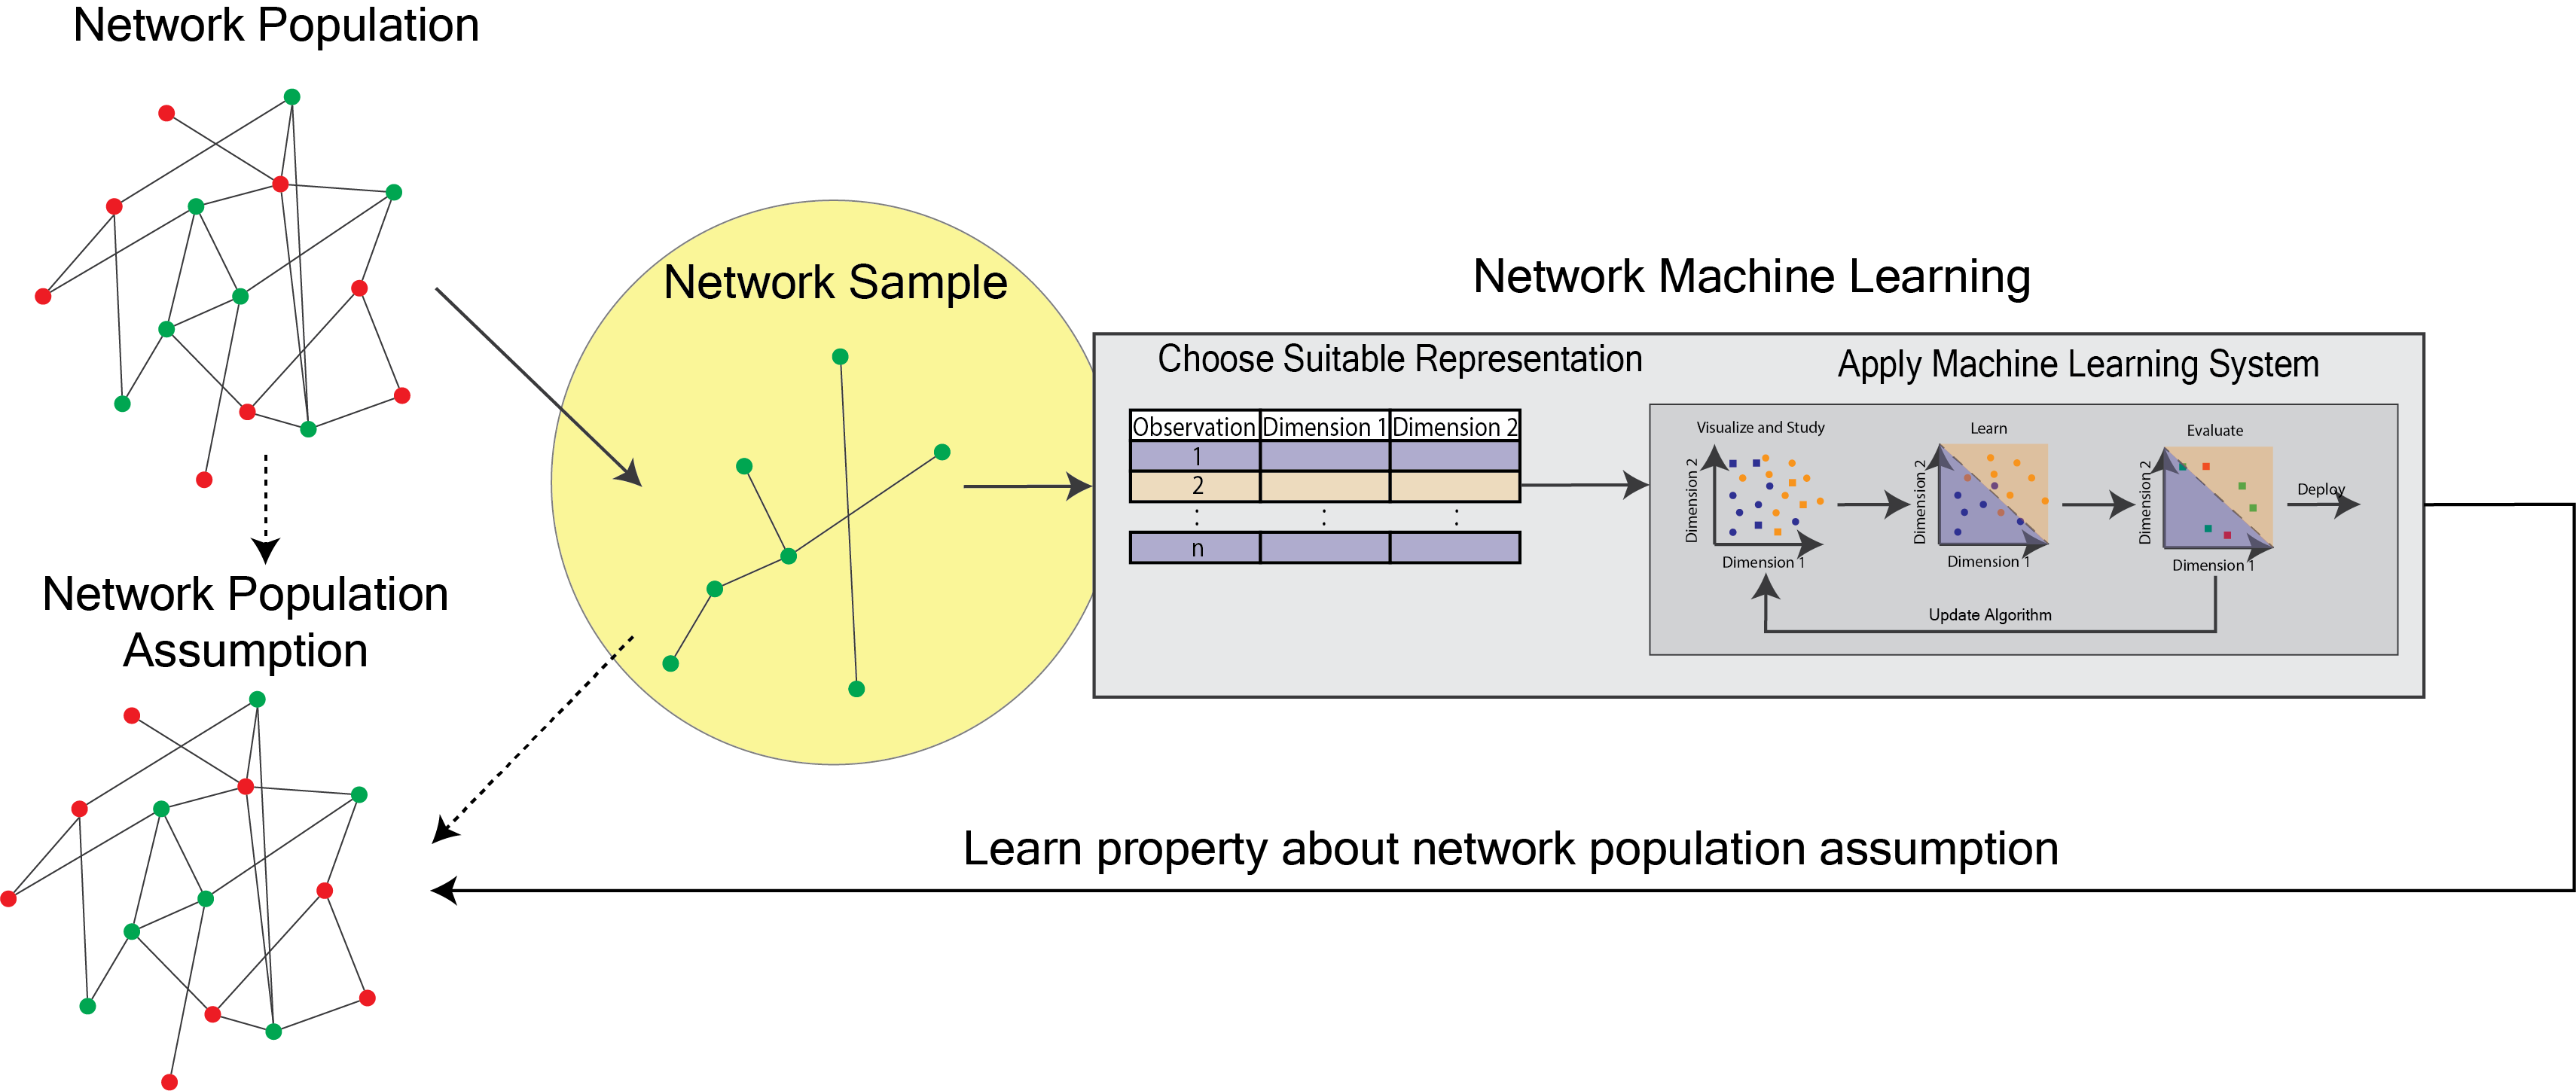
\includegraphics[width=\linewidth]{representations/ch4/Images/network_reps.png}
    \caption[Describing networks schematic]{The statistical learning pipeline. In this chapter, you will learn about how to describe the network you observe in your analysis.}
    \label{fig:ch4:rep_properties}
\end{figure}

When you try to learn from a network that you see through your research, your work, or anywhere else, the first thing to do is to know exactly how to describe that network. This network that you see is known as a {sample} or an {observation} of a network. The reason we call it an \emph{observation} or a \emph{sample} of a network is that the network you see is almost never going to {perfectly} describe the process you are trying to study. It is rarely the case that the network data you obtain will be perfect, as you learned in Section \ref{sec:ch1:challenges}. However, before we start to learn how to characterize that noise and perhaps better describe the observed network, you need to learn how to describe the network you observe first. 

Throughout the subsections, we'll learn about the fundamental representation we use for networks in this book, which is called the adjacency matrix. The reason we turn to adjacency matrices extremely often in network machine learning is that they tend to have nice mathematical properties; particularly, that the matrix is the fundamental unit for \emph{linear algebra}, a subset of mathematics that you might have become introduced to in your mathematical courses. When you apply algorithms to networks, more often than not, you can use \emph{linear algebra} techniques to describe the operation mathematically and in a precise way that allows you to apply the algorithm \emph{en masse} to the entire network.

\newpage 

\section{Matrix representations of networks}
\label{sec:ch4:mtx-rep}

When we work with networks, we need a way to represent them mathematically and in our code. A network itself lives in network space, which is just the set of all possible networks. Network space is kind of abstract and inconvenient if we want to use traditional mathematics, so we'd generally like to represent networks with groups of numbers to make everything more concrete.

More specifically, we would often like to represent networks with \emph{matrices}. In addition to being computationally convenient, using matrices to represent networks lets us bring in a surprising amount of tools from linear algebra and statistics. Programmatically, using matrices also lets us use common \texttt{python} tools for array manipulation like \texttt{numpy}.

For this section, we just wanted to get you acquainted with matrix representations of networks. This section will tie in directly with Section \ref{sec:ch4:prop-net}, so be aware that many of these concepts will be addressed in much more depth as the book progresses.

A common matrix representation of a network is called the Adjacency Matrix, and we'll learn about that first.

\subsection{Adjacency Matrices}

Throughout this book, the beating heart of matrix representations of networks that we will see is the adjacency matrix \cite{Godsil}. The idea is pretty straightforward: Let's say we have a network with $n$ nodes. We give each node an index (usually some value between $1$ and $n$, with one value per node) and then we create an $n \times n$ matrix. If there is an edge between node $i$ and node $j$, we fill the $(i, j)^{th}$ and $(j, i)^{th}$ values of the matrix with an entry, usually $1$ if our network has unweighted edges. In the case of undirected networks, we end up with a symmetric matrix with full of $1$s and $0$s, which completely represents the topology of our network.

Let's see this in action. We'll make a network with only three nodes, since that's small and easy to understand, and then we'll show what it looks like as an adjacency matrix. To visualize this network, we'll use something called a layout plot, provided by \texttt{nx.draw\_network()}.

\begin{lstlisting}[style=python]
import numpy as np
import networkx as nx

G = nx.DiGraph()
# add nodes to the network
G.add_node("1", pos=(1,1))
G.add_node("2", pos=(4,4))
G.add_node("3", pos=(4,2))
# add edges to the network
G.add_edge("1", "2")
G.add_edge("2", "1")
G.add_edge("1", "3")
G.add_edge("3", "1")

# the coordinates in space to use for plotting the nodes
# in the layout plot
pos = {'1': (0, 0), '2': (1, 0), '3': (.5, .5)}

nx.draw_networkx(G, with_labels=True, node_color="tab:purple", pos=pos,
                font_size=10, font_color="whitesmoke", arrows=False, edge_color="black",
                width=1)
\end{lstlisting}

The resulting plot of the network is shown in Figure \ref{fig:ch4:basic_mtxs}(A). Our network has three nodes, labeled $1$, $2$, and $3$. Each of these three nodes is either connected or not connected to each of the two other nodes. We'll make a square matrix $A$, with 3 rows and 3 columns, so that each node has its own row and column associated to it.

So, let's fill out the matrix. We start with the first row, which corresponds to the first node, and move along the columns. If there is an edge between the first node and the node whose index matches the current column, put a $1$ in the current location. If the two nodes aren't connected, add a $0$. When you're done with the first row, move on to the second. Keep going until the whole matrix is filled with $0$'s and $1$'s. 

Since the second and third nodes aren't connected, there is a $0$ in locations $a_{2, 1}$ and $a_{1, 2}$. There are also zeroes along the diagonals, since nodes don't have edges with themselves. In the plot, please take note of how we plotted the adjacency matrix using \texttt{heatmap()}; we won't always show you how to make this plot in the future. 

\begin{lstlisting}[style=python]
from graphbook_code import heatmap
import matplotlib.pyplot as plt
import seaborn as sns

# convert the networkx graph to a numpy array
A = np.asarray(nx.to_numpy_matrix(G))

heatmap(A, annot=True, linewidths=.1, cbar=False, 
        title="Adjacency matrix", xticklabels=[1,2,3], xtitle="Node", 
        yticklabels=[1,2,3], ytitle="Node"
       )


\end{lstlisting}

The resulting adjacency matrix is shown in Figure \ref{fig:ch4:basic_mtxs}(B). Although the adjacency matrix is straightforward and easy to understand, it isn't the only way to represent networks with matrices.

\begin{figure}[h]
    \centering
    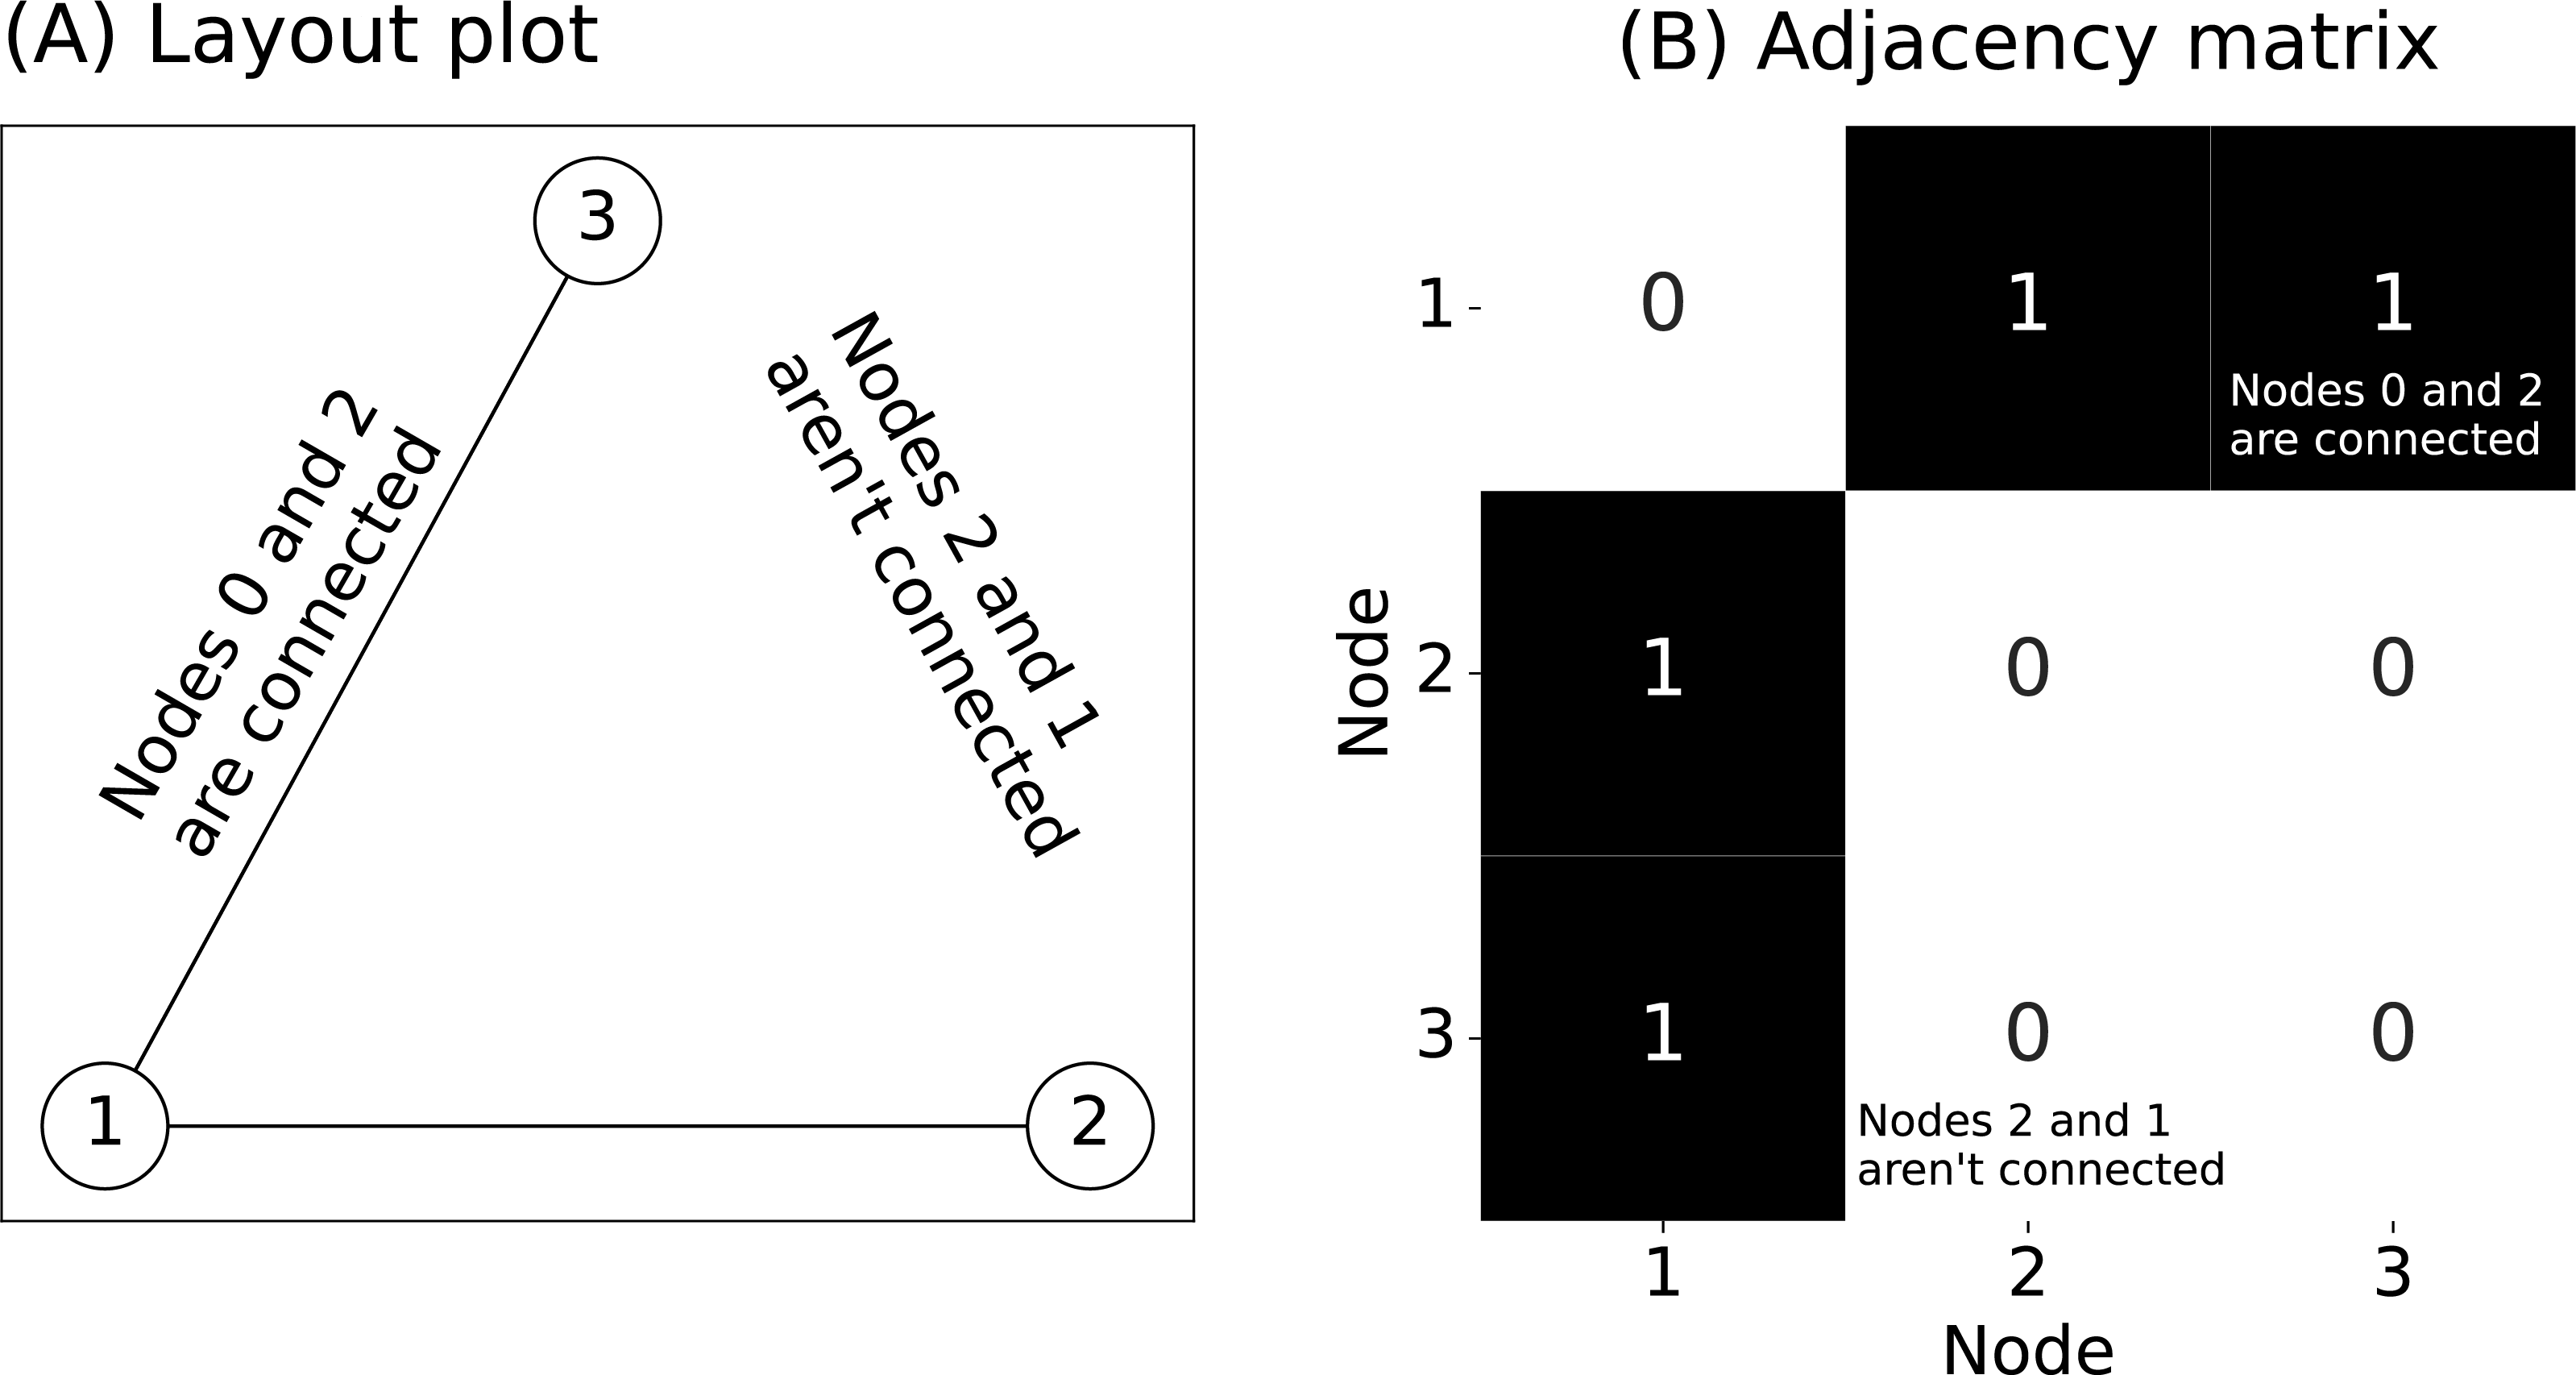
\includegraphics[width=0.8\linewidth]{representations/ch4/Images/basic_mtxs.png}
    \caption[Plotting a simple network as a layout plot and adjacency matrix heatmap]{\textbf{(A)} A layout plot of the network, where nodes are circles and edges are the lines connecting them. \textbf{(B)} the network, visualized as an adjacency matrix.}
    \label{fig:ch4:basic_mtxs}
\end{figure}

\subsection{The degree matrix}

The degree matrix isn't a full representation of our network, because we wouldn't be able to reconstruct an entire network from a degree matrix. However, it's fairly straightforward and it pops up relatively often as a step in creating other matrices, so the degree matrix is useful to mention. It's just a diagonal matrix with the values along the diagonal corresponding to the number of each edges each node has, also known as the \textit{degree} of each node. We'll learn more about the degree matrix in Section \ref{sec:ch4:prop-net}.

We can see the degree matrix for our network below. The diagonal element corresponding to node $1$ has the value of two, since it has two edges; the rest of the nodes have a value of $1$, since they each are only connected to the first node.

\begin{lstlisting}[style=python]
# Build the degree matrix D
degrees = np.count_nonzero(A, axis=0)
D = np.diag(degrees)
# plot it

heatmap(D, annot=True, linewidths=.1, cbar=False, 
        title="Degree matrix $D$", 
        xticklabels=[1,2,3], yticklabels=[1,2,3]
       ).set(xlabel="node", ylabel="node");

\end{lstlisting}
The degree matrix is shown in Figure \ref{fig:ch4:simple_lap}.

\subsection{The Laplacian Matrix}

The standard, cookie-cutter Laplacian Matrix $L$ \cite{Chung1996Dec} is just the adjacency matrix $A$ subtracted from the the degree matrix $D$:

\begin{align*}
 L = D - A
\end{align*}

Since the only nonzero values of the degree matrix is along its diagonals, and because the diagonals of an adjacency matrix never contain zeroes if its network doesn't have nodes connected to themselves, the diagonals of the Laplacian are just the degree of each node. The values on the non-diagonals work similarly to the adjacency matrix: they contain a $-1$ if there is an edge between the two nodes, and a $0$ if there is no edge.

The code below shows us what the Laplacian looks like. Since each node has exactly two edges, the degree matrix is just a diagonal matrix of all twos. The Laplacian looks like the degree matrix, but with -1's in all the locations where an edge exists between nodes $i$ and $j$. We can compute it using:

\begin{lstlisting}[style=python]
L = D - A
\end{lstlisting}

A plot of the Laplacian matrix as a heatmap, along with the degree and adjacency matrices, is shown in Figure \ref{fig:ch4:simple_lap}.
\begin{figure}[h]
    \centering
    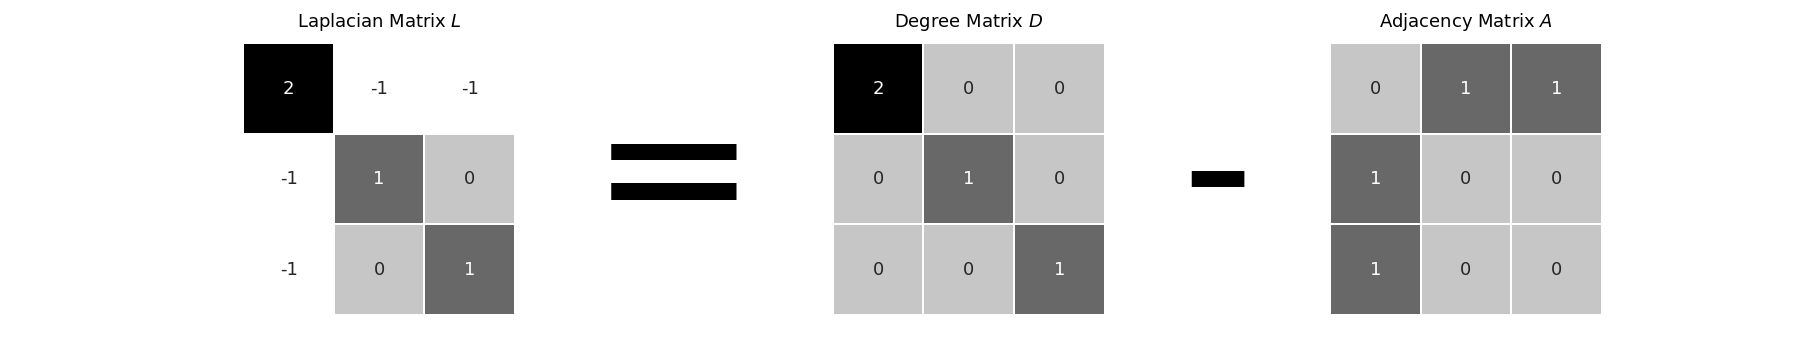
\includegraphics[width=\linewidth]{representations/ch4/Images/simple_lapl.png}
    \caption[Laplacian matrix]{The Laplacian matrix, along with the components that are used to compute it (the degree matrix and the adjacency matrix).}
    \label{fig:ch4:simple_lap}
\end{figure}

We use the Laplacian in practice because it has a number of interesting mathematical properties which tend to be useful for analysis. For instance, the magnitude of its second-smallest eigenvalue, called the Fiedler eigenvalue, tells us how well-connected our network is -- the number of eigenvalues equal to zero is the number of connected components our network has (a concept you will be introduced to in Section \ref{sec:ch4:prop-net:lcc}). Incidentally, this means that the smallest eigenvalue of the Laplacian will always be 0, since any simple network always has at least one ``island''. We don't need to have too much intuition for what eigenvalues mean, but just be aware that they will matter somewhat later on for now.

Another interesting property of the Laplacian is that the sum of its diagonals is twice the number of edges in the network. Because the sum of the diagonal matrix is the trace, and the trace is also equal to the sum of the eigenvalues, this means that the sum of the eigenvalues of the Laplacian is equal to twice the number of edges in the network.

Laplacians and adjacency matrices will be used throughout this book, and details about when and where one or the other will be used are in Chapter \ref{sec:ch6}.

\subsection{The Normalized Laplacian}
\label{sec:ch4:mat-rep:normlapl}

There are a few variations on the standard $D-A$ version of the Laplacian which are widely used in practice, and which (confusingly) are often also called the Laplacian. They tend to have similar properties. The Normalized Laplacian, $L^{norm.}$ is one such variation. The Normalized Laplacian \cite{Chung1996Dec} is defined as:

\begin{align*}
    L^{norm.} = D^{-1/2} L D^{-1/2} = I - D^{-1/2} A D^{-1/2}
\end{align*}

Where $I$ is the identity matrix (the square matrix with all zeroes except for ones along the diagonal). You can work through the algebra yourself if you'd like to verify that the second expression is the same as the third.

Below we can see the normalized Laplacian in code. We use \texttt{graspologic}'s \texttt{to\_laplacian()} function, with the \texttt{form} set to \texttt{I - DAD}, which computes $L^{norm.}$ above.
 
\begin{lstlisting}[style=python]
from graspologic.utils import to_laplacian
L_sym = to_laplacian(A, form="I-DAD")
\end{lstlisting}
A heatmap of the normalized Laplacian is shown in Figure \ref{fig:ch4:normlapl}(A).

We can understand the normalized Laplacian from the name: we can think of it as the Laplacian normalized by the degrees of the nodes associated with a given entry.

We can see this by looking at what the operation is doing:

\begin{align*}
    L^{norm.} &= D^{-\frac{1}{2}}L D^{-\frac{1}{2}} \\
    &= \begin{bmatrix}
        d_{1} & & \\
        & \ddots & \\
        & & d_n
    \end{bmatrix}^{-\frac{1}{2}}\begin{bmatrix}
        l_{11} & ... & l_{1n} \\
        \vdots & \ddots & \vdots \\
        l_{n1} & ... & l_{nn}
    \end{bmatrix}
    \begin{bmatrix}
        d_{1} & & \\
        & \ddots & \\
        & & d_n
    \end{bmatrix}^{-\frac{1}{2}} \\
    &= 
    \begin{bmatrix}
        \frac{1}{\sqrt{d_1}} & & \\
        & \ddots & \\
        & & \frac{1}{\sqrt{d_n}}
    \end{bmatrix}\begin{bmatrix}
        l_{11} & ... & l_{1n} \\
        \vdots & \ddots & \vdots \\
        l_{n1} & ... & l_{nn}
    \end{bmatrix}
    \begin{bmatrix}
        \frac{1}{\sqrt{d_1}} & & \\
        & \ddots & \\
        & & \frac{1}{\sqrt{d_n}}
    \end{bmatrix} \\
    &= \begin{bmatrix}
        \frac{l_{11}}{d_1} & ... & \frac{l_{1n}}{\sqrt{d_1}\sqrt{d_n}} \\
        \vdots & \ddots & \vdots \\
        \frac{l_{n1}}{\sqrt{d_n}\sqrt{d_1}} & ... & \frac{l_{nn}}{d_n}
    \end{bmatrix}
\end{align*}
So the normalized laplacian has entries $l^{norm.}_{ij} = \frac{l_{ij}}{\sqrt{d_i}\sqrt{d_j}}$.

We can plug in the value of $L$ to obtain a similar relationship with the adjacency matrix $A$. Notice that:
\begin{align*}
    L^{norm.} &=  D^{-\frac{1}{2}}L D^{-\frac{1}{2}} \\
    &=  D^{-\frac{1}{2}}(D - A) D^{-\frac{1}{2}} \\
    &= D^{-\frac{1}{2}}DD^{-\frac{1}{2}} - D^{-\frac{1}{2}}A D^{-\frac{1}{2}} \\
    &= D^{\frac{1}{2}}D^{-\frac{1}{2}} - D^{-\frac{1}{2}}A D^{-\frac{1}{2}} \\
    &= I_{n \times n} - D^{-\frac{1}{2}}A D^{-\frac{1}{2}}
\end{align*}

The $D^{-1/2} D D^{-1/2}$ term is spiritually the same as what we'd think of $\frac{D}{D}$ (if that was defined!), since it just works out to be the identity matrix. The $D^{-1/2} A D^{-1/2}$ is just doing the same thing to $A$ that we did to $L$. So we're normalizing the entries of the adjacency matrix by the degrees of the nodes a given entry is concerned with; that is, $\frac{a_{ij}}{\sqrt{d_i}\sqrt{d_j}}$.

One useful property of the normalized Laplacian is that its eigenvalues are bounded between 0 and 2. This normalization tends to be useful, because the Laplacian is a thing called a \emph{positive semi-definite matrix}. This means that a suite of linear algebra techniques, which may \emph{not} run successfully on the adjacency matrix (which is \emph{not} positive semi-definite in its most raw form for \emph{simple networks}, which we will learn about in the next chapter), can be executed on the network Laplacian. For more details about the properties of the Laplacian, check out \cite{Li2014Dec}.

\subsection{The \texttt{DAD} Laplacian}
\label{sec:ch4:mtx-rep:dad_laplacian}

In this book, a lot of what we will cover will be something called a \emph{spectral embedding} of the Laplacian. While we will learn all about this in Section \ref{sec:ch6:lse}, there are some fine points we want to cover here. As it turns out, there is another, \emph{related}, definition of a Laplacian, which we call the \texttt{DAD} Laplacian:

\begin{align*}
    L^{DAD} &= D^{-\frac{1}{2}}A D^{-\frac{1}{2}}
\end{align*}

$L^{DAD}$ and $L^{norm.}$ share some major similarities which are important to note here. Later in the book in Section \ref{sec:ch6:lse}, you will learn about the importance of the singular value decomposition for spectral embedding of Laplacians. Basically, what the singular value decomposition will allow us to do is look at the laplacian as a sum of much \emph{simpler} matrices. By ``simple'', what we mean here is that they can be represented as the product of two vectors. By looking only at the first few of these ``simple'' matrices, we can learn about the Laplacian and reduce a lot of noise in the Laplacian itself. The properties of looking at the \texttt{DAD} Laplacian are discussed at length in \cite{Chaudhuri2012Jun} and \cite{Amini2012Jul},

The most important connection is that these "simple" matrices will be \emph{identical} for $L^{norm.}$ and $L^{DAD}$, except for one important fact: they will be in \emph{reverse} order from one another. In $L^{norm}$, the matrices we will want to use will be the last few, and in $L^{DAD}$, the matrices we will want to use will be the first few. When we compute the singular value decomposition, there are ways to only compute the first few matrices without having to go through the trouble of computing \emph{all} of them, whereas the reverse is not true! To get the last few simple matrices, we would have to compute all of the preceding ones first. This means that to get the simple matrices we want, we can get much better computational performance using $L^{DAD}$ instead of $L^{norm}$.

We can compute the $L^{DAD}$ in \texttt{graspologic} similarly to above, but with \texttt{form="DAD"}:

\begin{lstlisting}[style=python]
L_dad = to_laplacian(A, form="DAD")
\end{lstlisting}

A heatmap of the \texttt{DAD} Laplacian is shown in Figure \ref{fig:ch4:normlapl}(B).

\subsection{The regularized Laplacian}
\label{ch4:mtx-rep:reg_laplacian}
The regularized Laplacian is an adaptation of the \texttt{DAD} Laplacian we learned about in the previous section. As it turns out, when networks have degree matrices where some of the degrees are really, really small, the \emph{spectral clustering} approach we will learn about in Section \ref{sec:ch7:comm_detect} is simply not going to perform very well. When we say it is not going to perform very well, what we mean is that the spectral clusterings are going to be extremely influenced by these nodes with really small node degrees. To overcome this hurdle, instead of using the \texttt{DAD} Laplacian, we can use the regularized Laplacian, defined extremely similarly to the \texttt{DAD} Laplacian, as:

\begin{align*}
    L^{rDAD}(\tau) &= D_\tau^{-\frac{1}{2}}A D_\tau^{-\frac{1}{2}}
\end{align*}

Where $\tau$ is a regularization constant which is greater than or equal to zero, and $D_\tau = D + \tau I$. When we put $\tau$ in parentheses here (that is, $(\tau)$), all that we mean is that $L^{rDAD}$ is a function of the particular regularization constant that we choose. Basically, what this is going to do is just "inflate" the diagonal elements of the degree matrix. So, if the degree for some of the nodes is extremely small, when we add a constant $\tau$ to them, we can increase the degrees by $\tau$. In effect, what this will do is make the nodes with really small degrees (which, like we said, might cause issues in the spectral clustering) a lot less impactful on the results that we obtain. Also, as we can see, if $\tau = 0$, then $L^{rDAD}(\tau) = L^{DAD}$. The regularized Laplacian is discussed at length in \cite{Qin2013Sep}.

Let's take a look at what $L^{rDAD}(\tau)$ and $L^{DAD}$ look like when we pick $\tau$ to be $1$. We can do this in \texttt{graspologic} using \texttt{form="R-DAD"}, and then setting \texttt{regularizer} appropriately:
\begin{lstlisting}[style=python]
tau = 1
L_rdad = to_laplacian(A, form="R-DAD", regularizer=tau)
\end{lstlisting}
The \texttt{R-DAD} Laplacian is shown in Figure \ref{fig:ch4:normlapl}(C).

We will learn about some other ways to handle nodes with very low degrees in Section \ref{sec:ch4:regularization} on Regularization.

\begin{figure}[h]
    \centering
    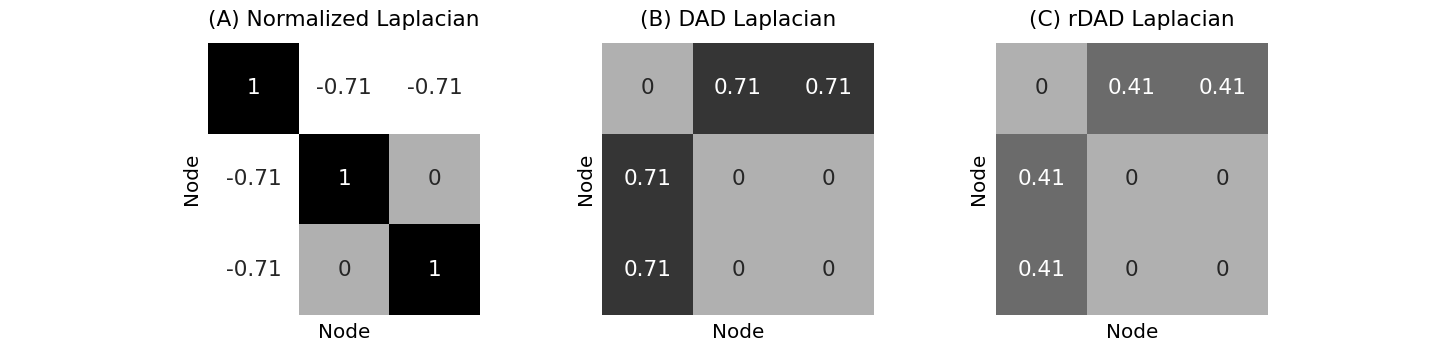
\includegraphics[width=\linewidth]{representations/ch4/Images/normlapls.png}
    \caption[comparison of normalized Laplacians]{Different variations of Laplacians for the same underlying network.}
    \label{fig:ch4:normlapl}
\end{figure}

\newpage
\section{Properties of networks}
\label{sec:ch4:prop-net}


\subsection{Descriptive Properties of Networks}

Remember that with a network, we can represent the collection of nodes and edges as an $n \times n$ adjacency matrix, where $n$ is the total number of nodes. The adjacency matrix looks like this:

\begin{align*}
    A &= \begin{bmatrix}
        a_{11} & ... & a_{1n} \\
        \vdots & \ddots & \vdots \\
        a_{n1} & ... & a_{nn}
    \end{bmatrix},
\end{align*}

Let's say you have a network representing the five boroughs of New York (Staten Island SI, Brooklyn BK, Queens Q, the Bronx BX, and Manhattan MH). The nodes in your network are the five boroughs. The edges $(i,j)$ of your network exist if one can travel from borough $i$ to borough $j$ along a bridge. Let's start by defining a network for ourselves with \texttt{networkx}'s \texttt{DiGraph()} function:


\begin{lstlisting}[style=python]
import networkx as nx
from graphbook_code import heatmap

# create an undirected network G
G = nx.Graph()
# add the nodes like before
G.add_node("SI", pos=(2,1))
G.add_node("MH", pos=(4,4))
G.add_node("BK", pos=(4,1.7))
G.add_node("Q", pos=(6,3))
G.add_node("BX", pos=(6,6))

# specify boroughs that are connected to one another
pos = nx.get_node_attributes(G, 'pos')
G.add_edge("SI", "BK")
G.add_edge("MH", "BK")
G.add_edge("MH", "Q")
G.add_edge("MH", "BX")
G.add_edge("Q", "BX")

A = nx.to_numpy_array(G)

# plotting
nx.draw_networkx(G, with_labels=True, node_color="black", pos=pos,
                font_color="white", edge_color="black")

# pass in the xticklabels and yticklabels corresponding to the
# appropriately ordered boroughs (in the order we constructed them)
heatmap(A.astype(int), xticklabels=["SI", "MH", "BK", "Q", "BX"],
            yticklabels=["SI", "MH", "BK", "Q", "BX"], 
       ).set(xlabel="Borough", ylabel="Borough")
\end{lstlisting}

Figure \ref{fig:ch4:nyc_ex} shows a plot of the bridges of New York, a layout plot representation of a network derived from the the boroughs of New York, and an adjacency matrix as a heatmap of this network.

In this section, we're going to discuss a number of descriptive measures and summary statistics about networks. For a detailed overview, there are a lot of great references out there; some of our favorites are \cite{Barabsi2013Mar}, \cite{Gross2005Sep}, and \cite{Newman2006Jun}, to name a few.

\begin{figure}
    \centering
    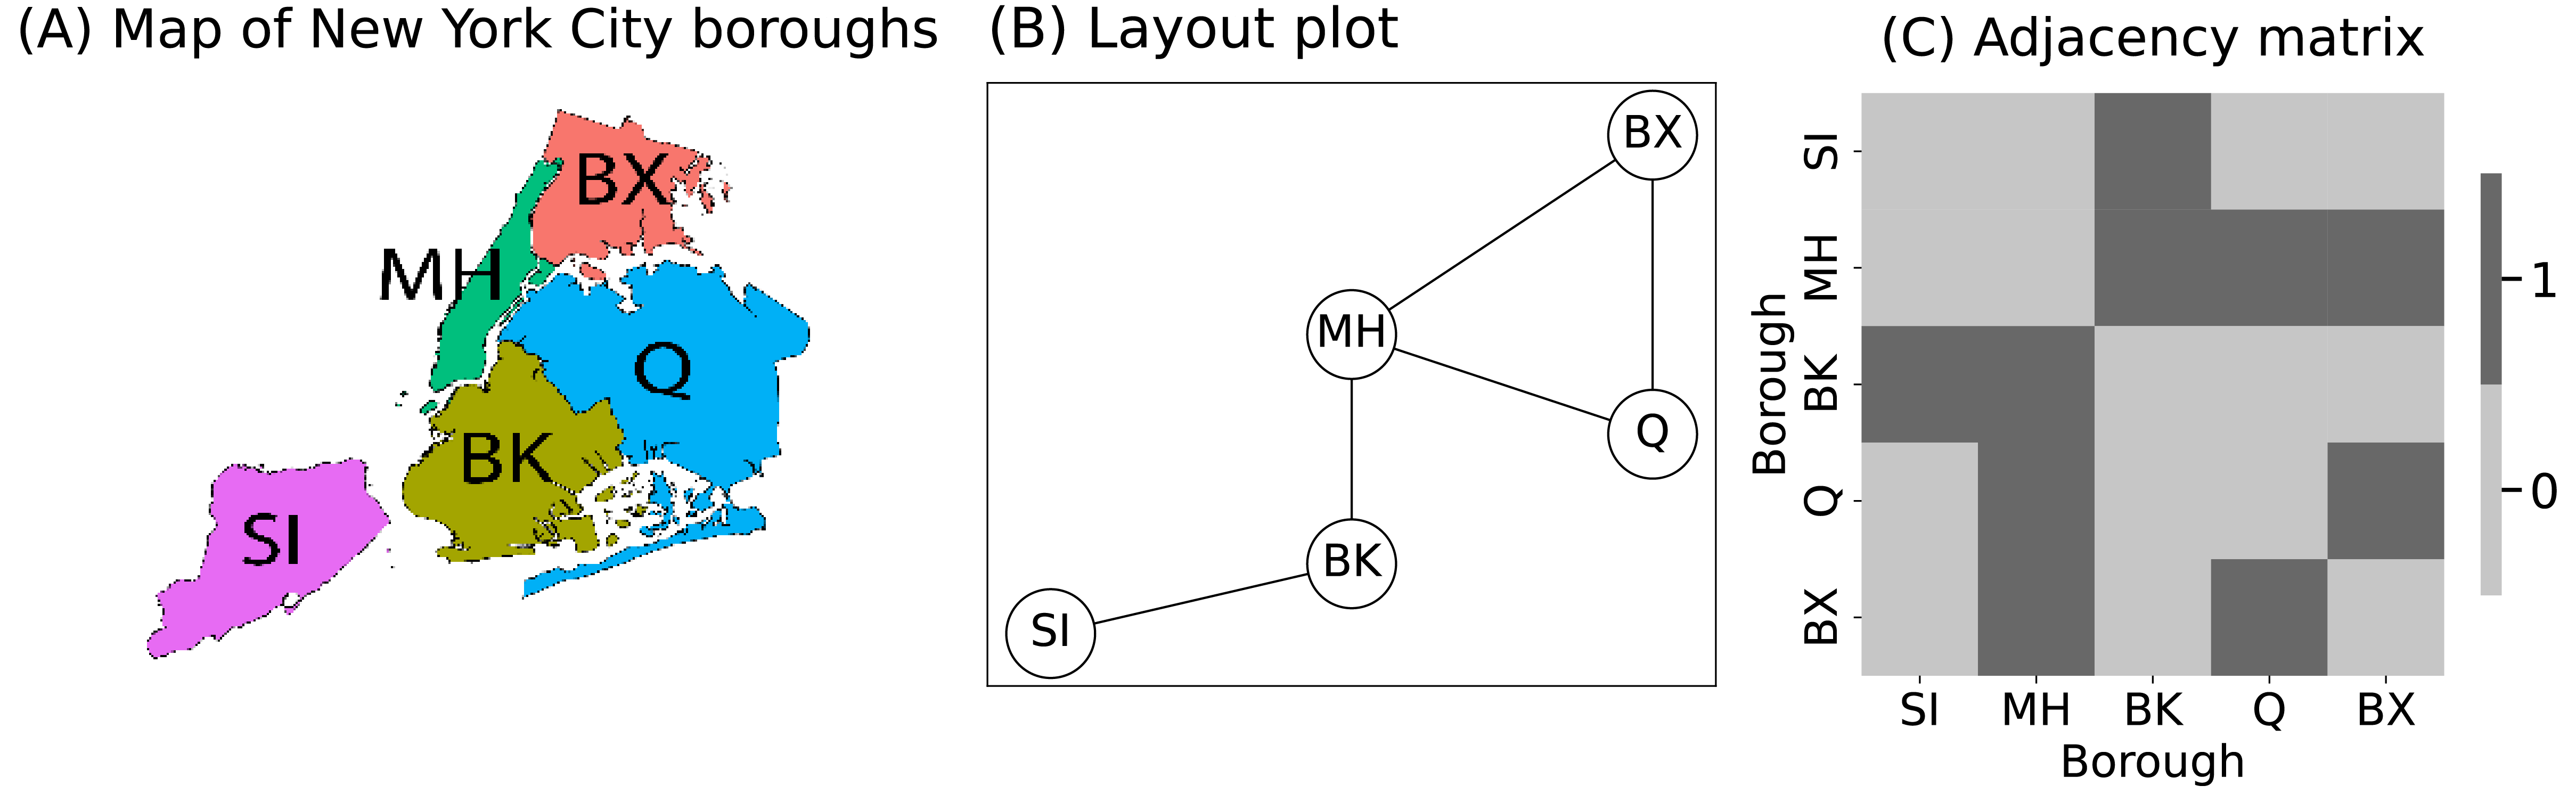
\includegraphics[width=\linewidth]{representations/ch4/Images/nyc_ex.png}
    \caption[New York City borough example]{\textbf{(A)} a map of New York, with the bridges that connect different boroughs. We use this to construct a network of New York, where the nodes are boroughs of New York and the edges are bridges between different boroughs. \textbf{(B)} the network visualized as a layout plot. \textbf{(C)} the network visualized as a heatmap.}
    \label{fig:ch4:nyc_ex}
\end{figure}

\subsection{The edges of undirected networks are bi-directional}

When you decide to travel from borough $i$ to borough $j$, you care about whether you can {actually drive} in that direction. In a similar way, the concept of directedness describes whether you need to worry about one-way bridges and bridge closures. If your network contains one-way bridges, then a bridge from borough $i$ to borough $j$ doesn't {necessarily} imply that a bridge from borough $j$ to borough $i$ exists (just ask New York drivers). If, for instance, the Brooklyn bridge was closed from Brooklyn to Manhattan, your network might change like this. Note that there is no arrow going from Brooklyn to Manhattan, so you cannot drive directly from MH to BK. We can do this by removing the edge from MH to BK:

\begin{lstlisting}[style=python]
from copy import deepcopy

G_dir = G.to_directed()
# remove the edge from MH to BK
G_dir.remove_edge("BK", "MH")

nx.draw_networkx(G_dir, with_labels=True, node_color="black", pos=pos,
                font_color="white", arrows=True, edge_color="black")
\end{lstlisting}

Basically, the arrows of the directed network tell you which nodes you can travel between. Note that we passed the \texttt{arrows="True"} argument, which tells \texttt{networkx} to include the arrows in our plot. A plot of this network is shown in Figure \ref{fig:ch4:directed}(B). Note that there are bi-directional arrows (arrows from one node to the other, as well as the reverse) for all pairs of nodes except Brooklyn and Manhattan.

\begin{figure}[h]
    \centering
    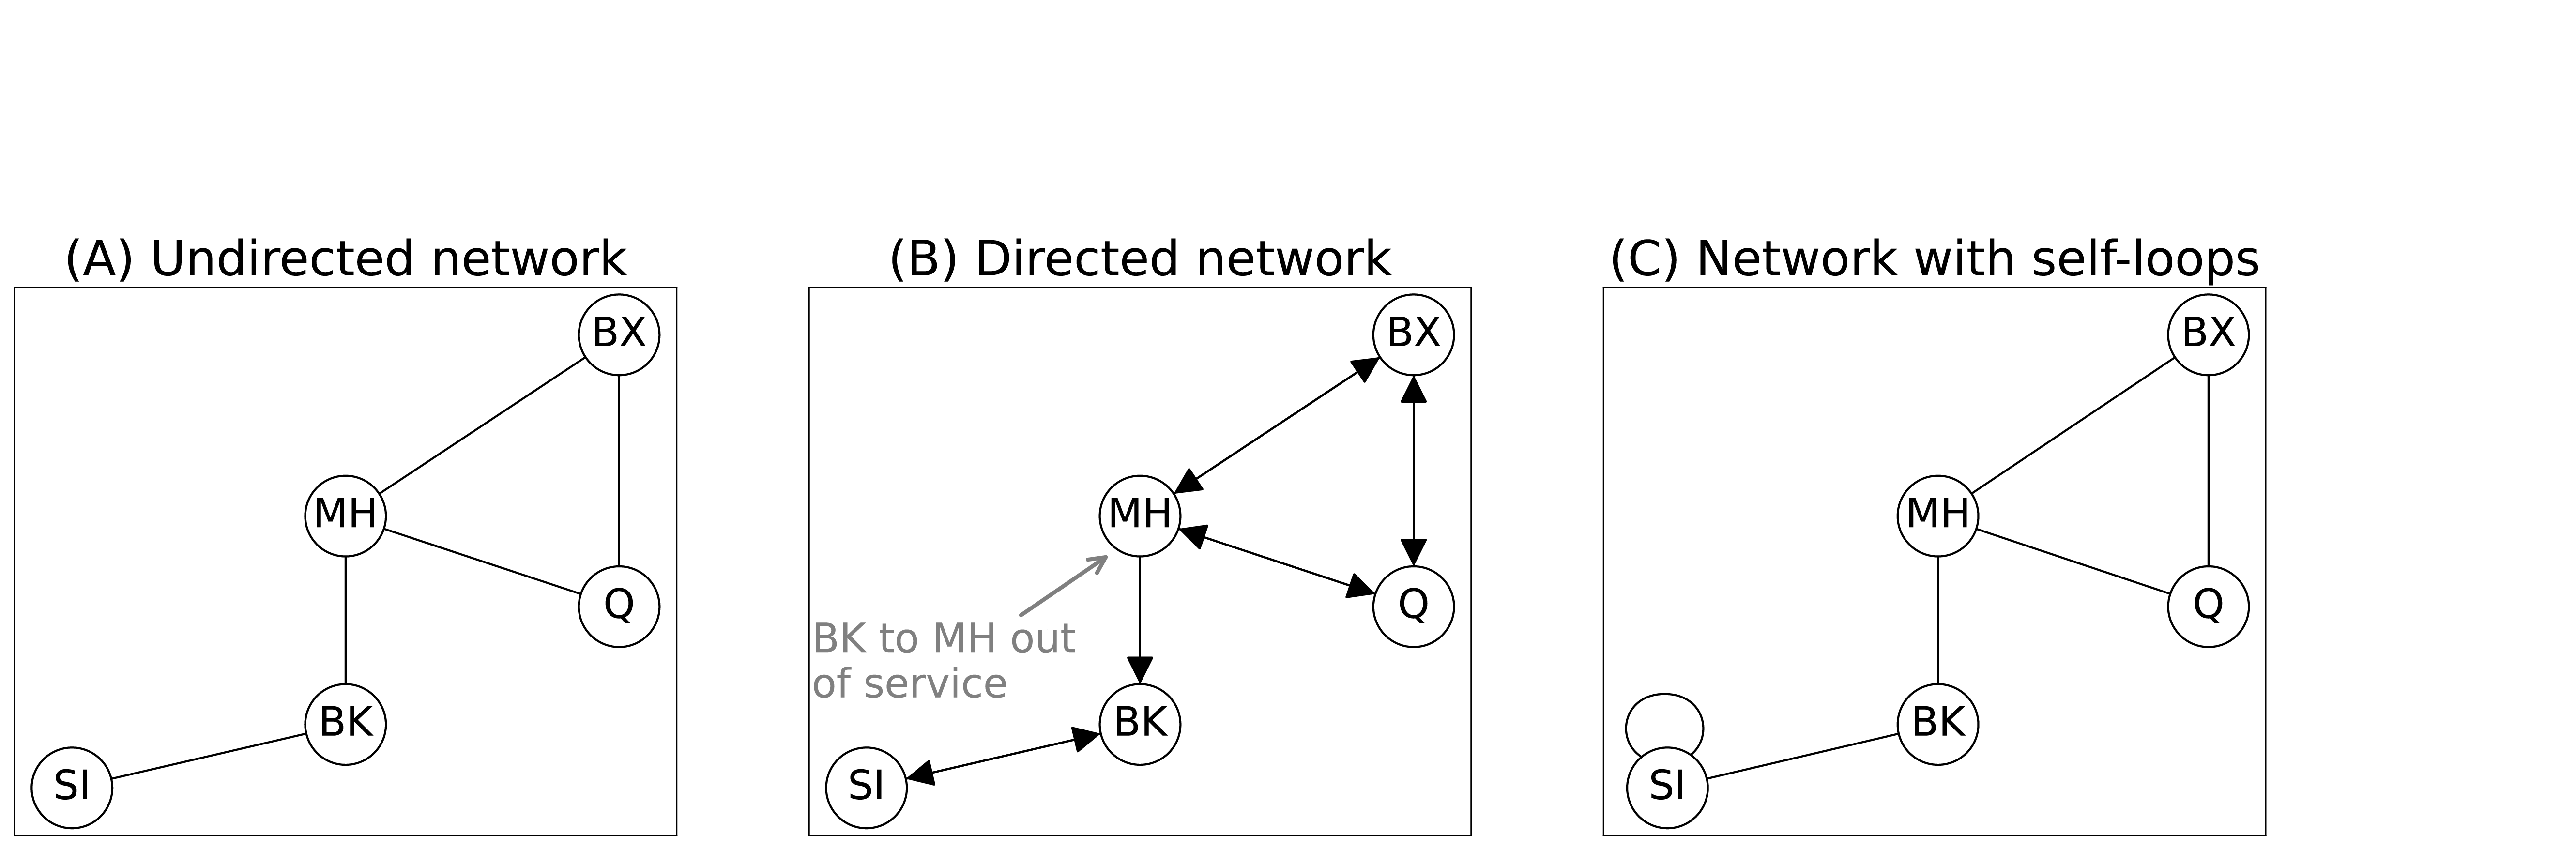
\includegraphics[width=\linewidth]{representations/ch4/Images/directed.png}
    \caption[Comparing directed and undirected networks]{\textbf{(A)} The undirected network. \textbf{(B)} A plot of the network with the bridge from BK to MH out of service. \textbf{(C)} a plot of the network with a self-loop.}
    \label{fig:ch4:directed}
\end{figure}

In the context of this book, we will usually only worry about the undirected case, or when the presence of an arrow implies that the other direction exists, too. A network is \textit{undirected} if an edge between node $i$ and node $j$ implies that node $j$ is also connected to node $i$. 

A plot of the undirected network is shown in Figure \ref{fig:ch4:directed}(A). For the adjacency matrix $A$, remember an edge between nodes $i$ and $j$ is represented by the adjacency $a_{ij}$. This means that if the network is undirected, $a_{ij} = a_{ji}$, for all pairs of nodes $i$ and $j$. By definition, this tells us that the adjacency matrix $A$ is \textit{symmetric}, so $A = A^\top$. We can verify this condition with \texttt{graspologic}:
\begin{lstlisting}[style=python]
from graspologic.utils import is_symmetric

A = nx.to_numpy_array(G)
is_symmetric(A)
# True
A_dir = nx.to_numpy_array(G_dir)
is_symmetric(A_dir)
# False
\end{lstlisting}

\subsubsection{Loopless networks do not have self-loops}

If you are already in a borough, why would you want to take a bridge to that same borough? This logic relates to the concept of {self-loops} in a network. A \textit{self-loop} in a network describes whether nodes can connect back to themselves. For instance, consider the following loop on Staten Island. This would have the interpretation of a bridge which connects Staten Island back to itself:
\begin{lstlisting}[style=python]
G_loopy = deepcopy(G)
# add edge from SI to itself
G_loopy.add_edge("SI", "SI")
nx.draw_networkx(G_loopy, with_labels=True, node_color="black", pos=pos,
                font_color="white", edge_color="black")
\end{lstlisting}

A plot of this network is shown in Figure \ref{fig:ch4:directed}(C). A network is \textit{loopless} if self-loops are not possible. It is also important to note that both directed and undirected network can have self-loops; we only show the undirected case.

For the adjacency matrix $A$, a self-loop would be represented by the adjacencies $a_{ii}$ for all nodes $i$. Note that these entries $a_{ii}$ are all of the {diagonal} entries of $A$. Therefore, for a network which is loopless, all adjacencies $a_{ii}$ on the diagonal {do not exist}. Mathematically, we will represent this by saying that the diagonal entries are $0$, which means that the matrix is \textit{hollow}. You might also see this property abbreviated by stating that the diagonal of the adjacency matrix is $0$, or $diag(A) = 0$. It is important to understand that if the network is loopless, there is a theoretical distinction between $0$ and {does not exist}. Denoting the diagonal in an adjacency matrix of a loopless network with $0$ is a convenience and a convention for the field. This distinction will make a difference in later sections of this chapter, so be ready!

We can verify this condition using: 

\begin{lstlisting}[style=python]
from graspologic.utils import is_loopless
is_loopless(A)
# True
A_loopy = nx.to_numpy_array(G_loopy)
is_loopless(A_loopy)
# False
\end{lstlisting}


\subsubsection{Unweighted networks either have an edge, or they don't}

Do you need to convey information about how long it takes to get from borough $i$ to borough $j$ with your network? The broader fundamental question here -- whether an edge needs to carry extra information besides its existence -- underlies the concept of {weightedness} in networks. In a weighted network, you could use {edge-weights} $w(i, j)$ to describe the amount of time it takes to get from borough $i$ to borough $j$. An \textit{edge-weight} $w(i,j)$ assigns a weight to an edge between nodes $i$ and $j$ if that edge exists. If you care about weightedness in the network, the network is called {weighted}. 

The potential edges $a_{ij}$ of $A$ for a weighted network take the value of the edge-weight; that is, $a_{ij} = w(i, j)$ for any edge which exists between nodes $i$ and $j$. In the below plot, edge-weight indicates the approximate time to travel from one borough to the other. The network is undirected, so you don't have to worry about directionality differences. The edge-weight is indicated by the number along the corresponding edge.

\begin{lstlisting}[style=python]
G_weight = nx.Graph()

G_weight.add_node("SI", pos=(2,1))
G_weight.add_node("MH", pos=(4,4))
G_weight.add_node("BK", pos=(4,1.7))
G_weight.add_node("Q", pos=(6,3))
G_weight.add_node("BX", pos=(6,6))

# this time, we add weights to the edges
pos = nx.get_node_attributes(G, 'pos')
G_weight.add_edge("SI", "BK", weight=20)
G_weight.add_edge("MH", "BK", weight=15)
G_weight.add_edge("MH", "Q", weight=15)
G_weight.add_edge("MH", "BX", weight=5)
G_weight.add_edge("Q", "BX", weight=15)

A_weight = nx.to_numpy_array(G_weight)

nx.draw_networkx(G_weight, with_labels=True, node_color="black", pos=pos,
                 font_color="white", edge_color="black")

heatmap(A_weight, xticklabels=["SI", "MH", "BK", "Q", "BX"],
        yticklabels=["SI", "MH", "BK", "Q", "BX"], title="Weighted adjacency matrix", 
        font_scale=1.3, xtitle="Borough", ytitle="Borough")
\end{lstlisting}
We can identify whether a network is unweighted using \texttt{is\_unweighted()}:


\begin{lstlisting}[style=python]
from graspologic.utils import is_unweighted

A_weight = nx.to_numpy_array(G_weight)
is_unweighted(A)
# True
is_unweighted(A_weight)
# False
\end{lstlisting}
In a lot of your data analyses, you will come across weighted networks, so we give you an example of what they will look like in Figure \ref{fig:ch4:weighted}.

For most examples in this book, you will usually discuss {unweighted} or {binary} networks. A network is \textit{unweighted} or \textit{binary} if you only care about whether edges are {present} or {absent}. In an unweighted network, a potential edge $a_{ij}$ takes the value $1$ if there is an edge from node $i$ to node $j$, and takes the value $0$ if there is {not} an edge from node $i$ to node $j$.

\begin{figure}
    \centering
    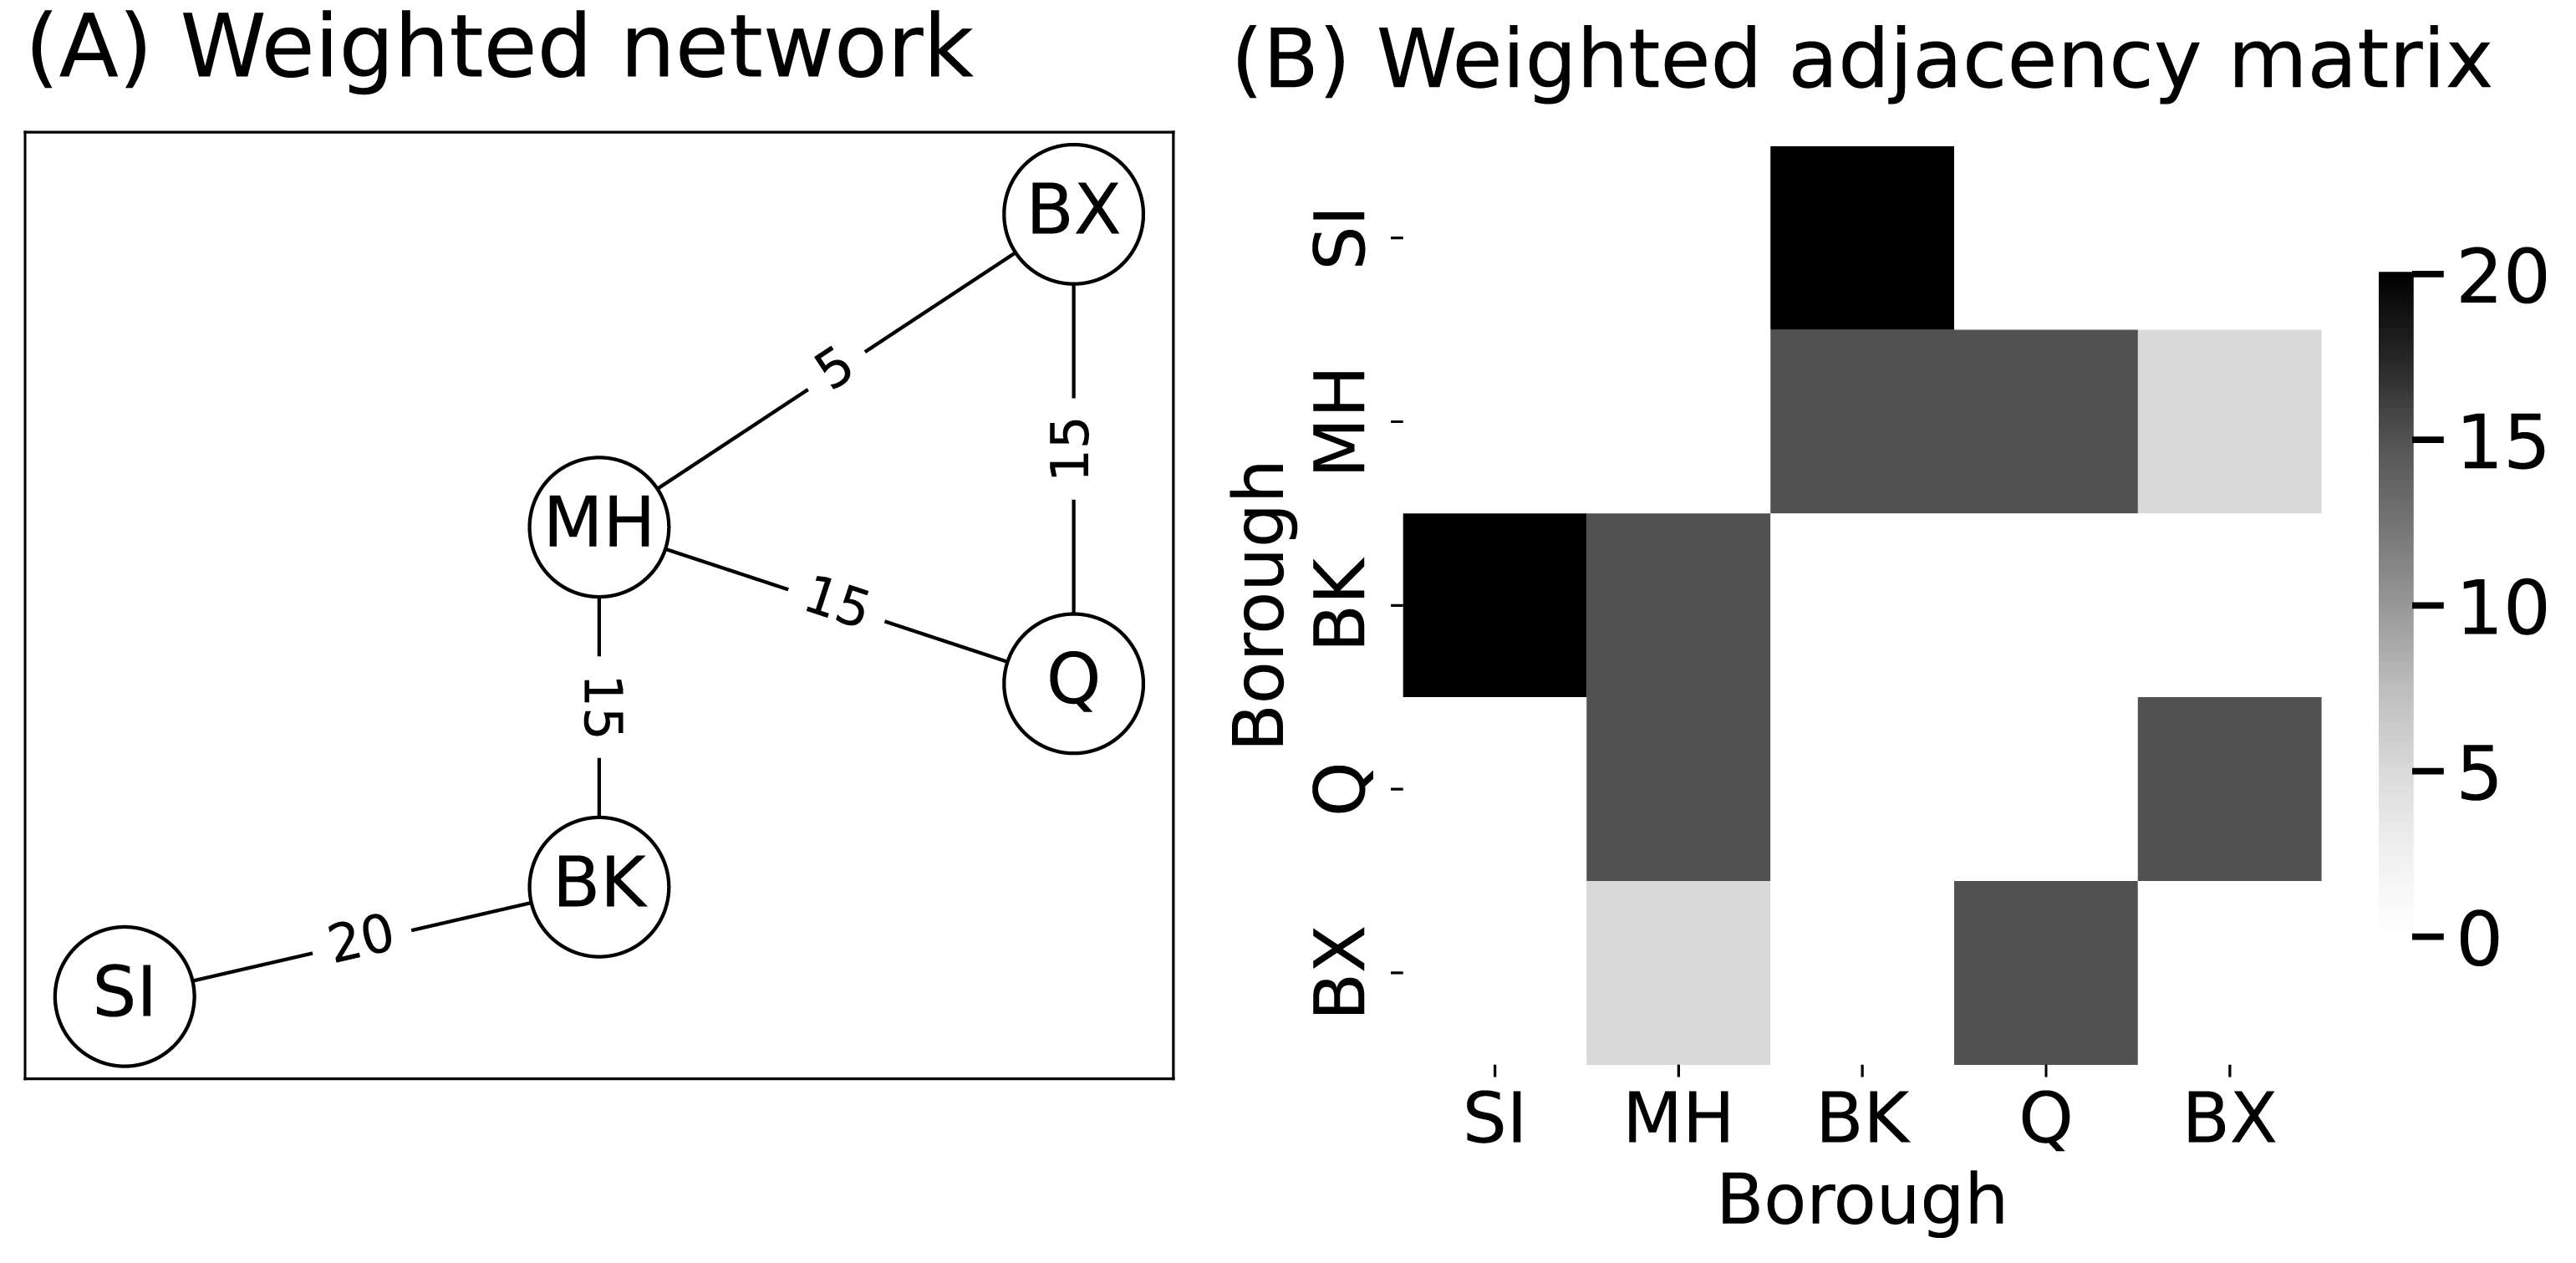
\includegraphics[width=0.8\linewidth]{representations/ch4/Images/weighted.png}
    \caption[Weighted network in New York borough example]{The New York City borough network, where weights indicate the travel times across the indicated bridges. \textbf{(A)} a layout plot for the weighted network, and \textbf{(B)} a heatmap of an adjacency matrix for the weighted network.}
    \label{fig:ch4:weighted}
\end{figure}

\begin{floatingbox}[h]\caption{This book considers {simple networks}}
A \textit{simple network} is loopless, undirected, and unweighted. Most of the examples and techniques you look at in this book are developed in the context of simple networks. Fortunately, this note is largely conceptual, and doesn't really impact much from an implementation perspective. All the techniques and packages you use will make sensible choices, or will directly extend, to cases that fall outside of this particular setup. If your networks don't satisfy one or any of these properties, most of the approaches discussed herein will still work. 

If the technique will not work for the network you have provided, the software package used (such as \texttt{networkx}, \texttt{graspologic}, or \texttt{igraph}) will probably either give you a warning or an explicit error if there is a substantial issue with the network you have provided. That said, when implementing network analysis methods on your own, we strongly encourage you to double check with the documentation to ensure that it is {compatible} with the type of network you are analyzing.
\end{floatingbox}

\subsection{Descriptive Properties of Nodes}

Just like you have many words and properties which describe the network itself, you also have special vocabulary in network machine learning to describe properties about the individual nodes in the network. We'll learn some of the ones here that will come up again later in the book.

\subsubsection{Node neighbors and incidences}

You begin by describing properties of single nodes in a simple network. The simplest property of a network is {adjacency}. A pair of nodes $i$ and $j$ in an undirected network are \textit{neighbors} if an edge exists between them. In terms of the adjacency matrix, two nodes $i$ and $j$ are neighbors if the potential edge $a_{ij}$ is one.

\subsubsection{Node degree quantifies the number of edges}
\label{sec:ch4:prop-net:degree}
The simplest summary statistic for a node is known as the {node degree}. The \textit{node degree} of $i$ in a simple network is the number of nodes with which it is a neighbor. Remember that if two nodes are not neighbors, the adjacency matrix entry corresponding to this {potential} edge takes a value of zero. This means that we can just count the potential edges $a_{ij}$ for a node $i$ to get its degree. We do this by just summing the $i^{th}$ row (or equivalently, if the network is simple, its $i^{th}$ column):

\begin{align}
    d_i &= degree(i) \triangleq \sum_{j = 1}^n a_{ij} = \sum_{j = 1}^n a_{ji}\label{eqn:ch4:degree}
\end{align}

Now you might be thinking, this isn't just counting edges which exist, since it counts {every} potential edge for node $i$. Let's see how that holds up. Remember that if an edge exists, $a_{ij}$ takes a value of $1$, whereas if an edge does not exist, $a_{ij}$ takes a value of $0$. This means that every $a_{ij}$ is either zero or one, so you can write:

\begin{align*}
    d_i &= \sum_{j = 1}^n a_{ij} \\
    &= \sum_{j : a_{ij} = 1} a_{ij} + \sum_{j : a_{ij} = 0}a_{ij} \\
    &= \sum_{j : a_{ij} = 1}1 + 0
\end{align*}
Note that in the left sum, since every $a_{ij}$ is defined to be one, that this is just the number of times that $a_{ij}$ takes a value of one, which is all of the edges that node $i$ touches. The right sum has every $a_{ij}$ defined to be zero, so this is just zero!

For instance, if you consider the node BK in your example, BK touches two edges, indicated in bold in  Figure \ref{fig:ch4:degree}(A), so $degree({BK}) = 2$. When you look at the corresponding adjacency matrix, if you sum the entries for node ${BK}$, you also get two. The entries which would be summed row-wise or column wise for ${BK}$ are shown in black boxes, in Figure \ref{fig:ch4:degree}(B).

\begin{figure}[h]
    \centering
    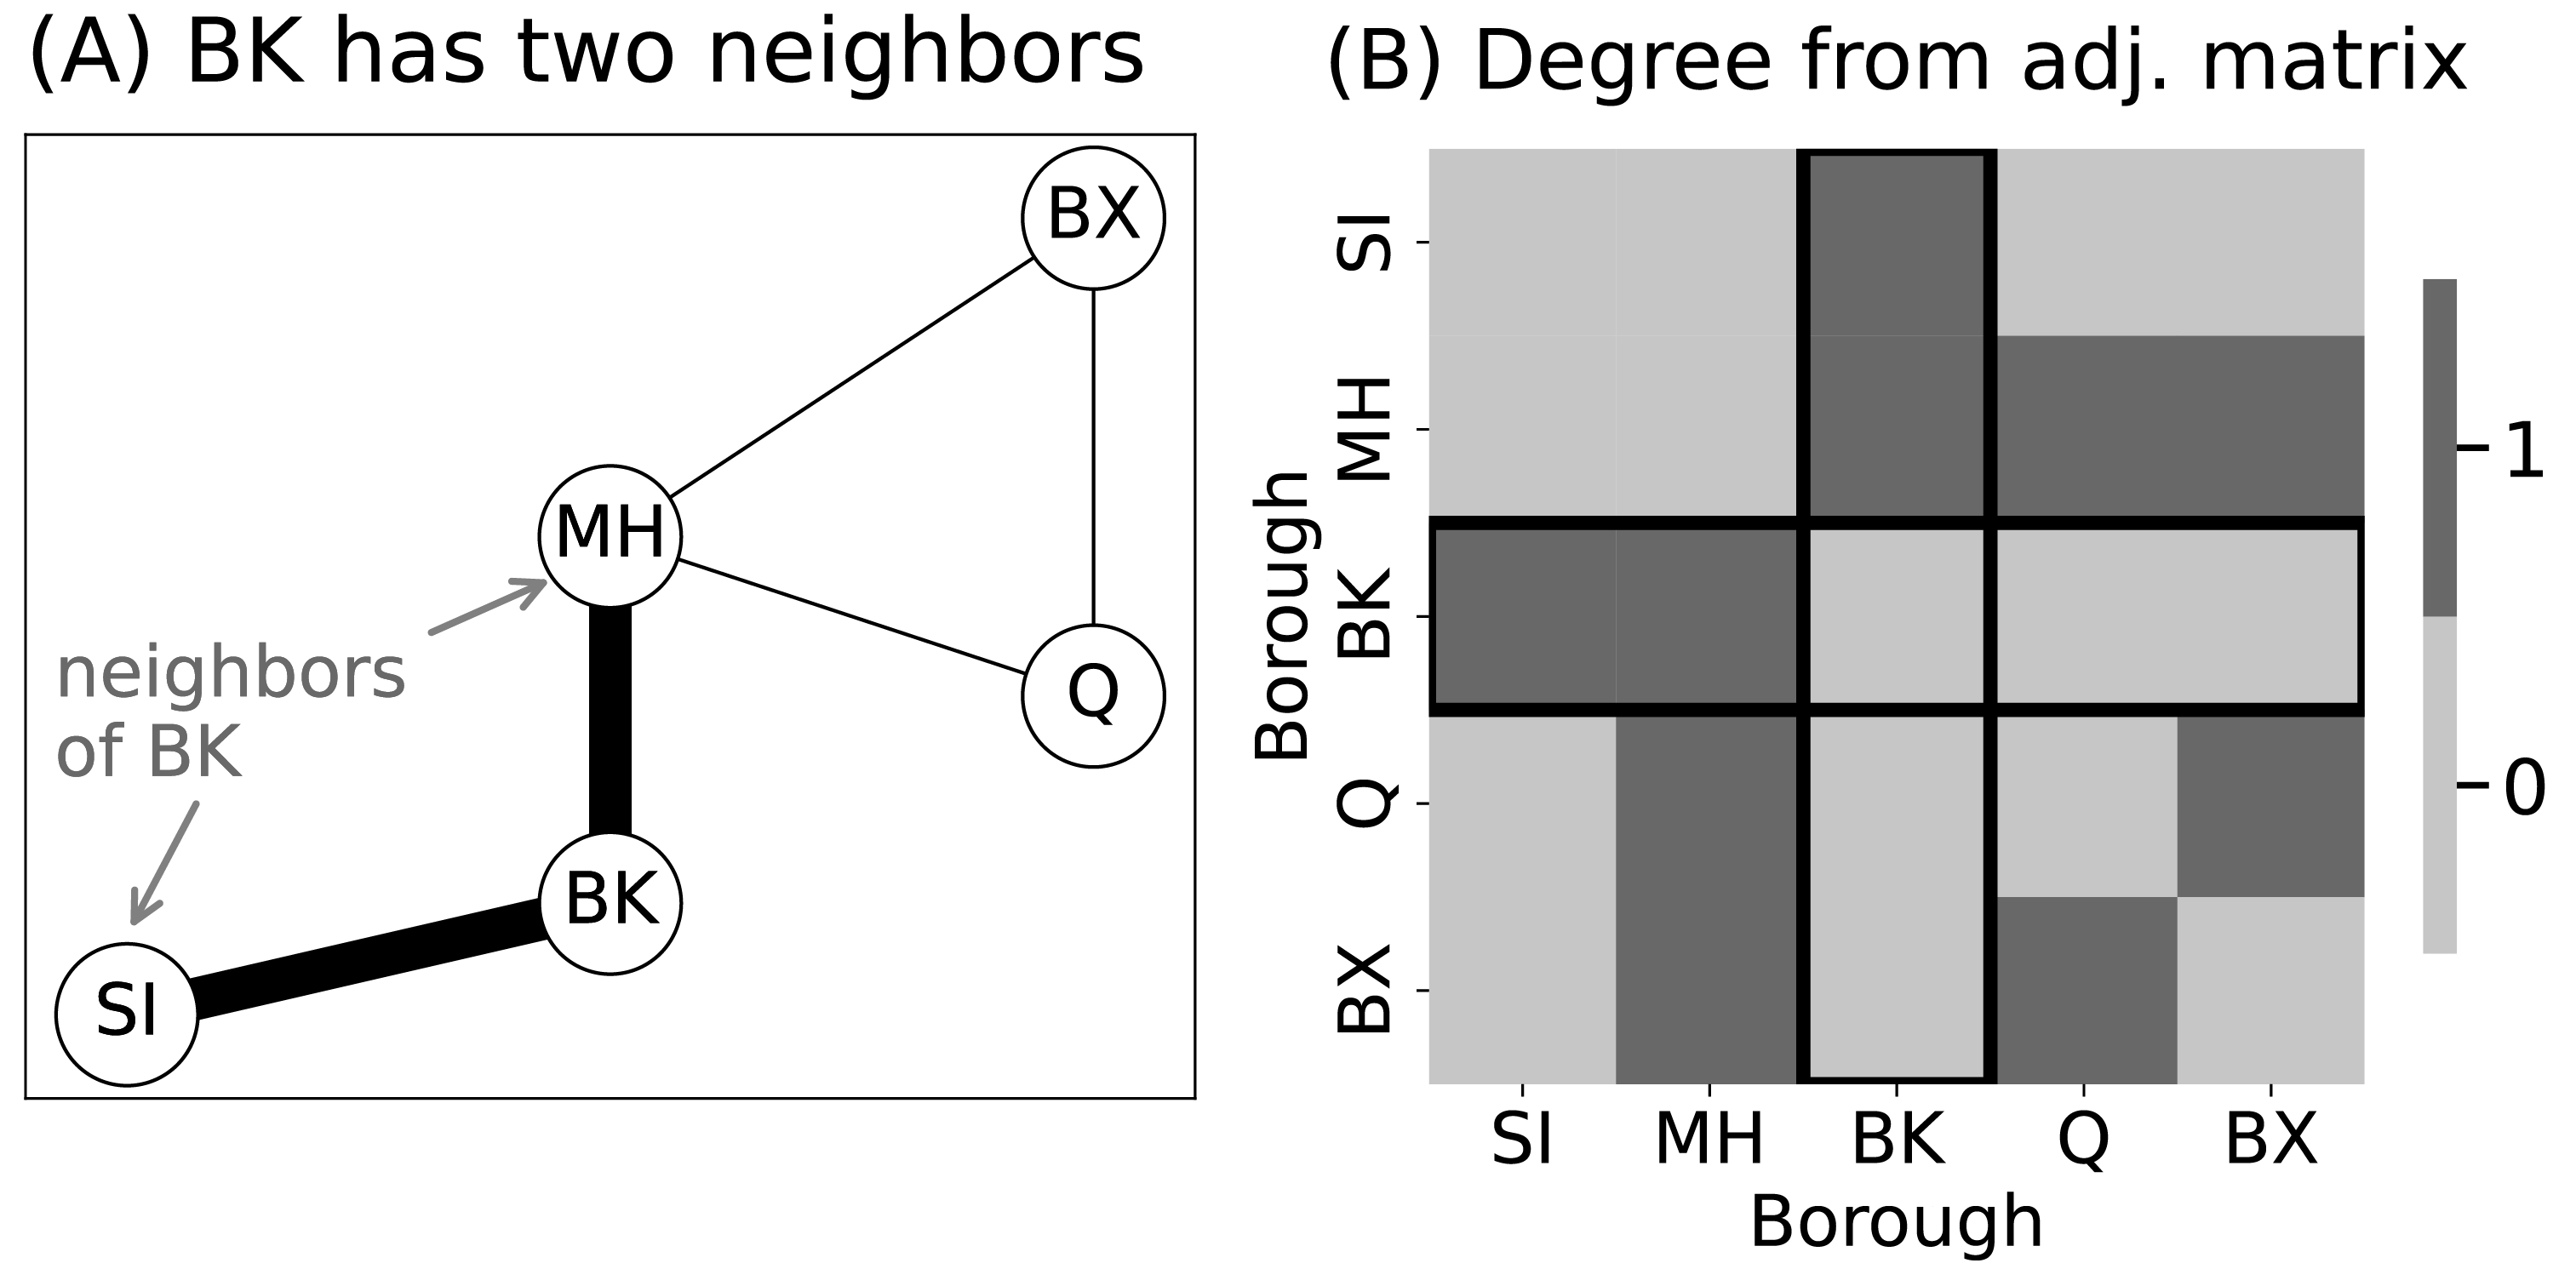
\includegraphics[width=0.8\linewidth]{representations/ch4/Images/degree.png}
    \caption[Deriving node degree from layout and adjacency matrix heatmaps]{A case-study of the BK borough. \textbf{(A)} shows that BK has two neighbors, SI and MH (edges to SI/MH are bold-faced). \textbf{(B)} shows the axes of the adjacency matrix could be summed to derive this fact as well. Note the row/column corresponding to BK (black boxes) has a sum value of two.}
    \label{fig:ch4:degree}
\end{figure}

It really doesn't matter whether you sum row or column-wise, as long as you pick one, if the network is undirected.

\subsubsection{The degree matrix indicates the degrees of each node}

A useful quantity which you will come across in many of the later chapters of this book is called the {degree matrix} of the network. The degree matrix is the {diagonal} matrix:
\begin{align*}
    D &= \begin{bmatrix}
        d_1 & 0 & ... & 0 \\
        0 & \ddots & \ddots& \vdots \\
        \vdots & \ddots & \ddots & 0 \\
        0 & ... & 0 & d_n
    \end{bmatrix}, \;\;\; d_i = degree(i)
\end{align*}
This matrix $D$ is called \textit{diagonal} because all of the entries $d_{ij} = 0$ unless $i = j$. The diagonal entries $d_{ii}$ of the degree matrix are simply the node degrees $degree(i)$ for each node $i$. Using the counting procedure you described above, you can see that the node SI has degree one, the node BK has degree two, the node MH has degree three, the node Q has degree two, and the node BX has degree two. We can compute the degree matrix for an unweighted network by using either of the following commands:

\begin{lstlisting}[style=python]
# summing column-wise
D_column = np.diag(A.sum(axis=0))
# summing row-wise
D_row = np.diag(A.sum(axis=1))
\end{lstlisting}

You can plot the degree matrix using the \texttt{heatmap} utility that we developed for the adjacency matrix.

\paragraph{Degrees for directed networks}

A question you might have in the back of your head is, "what if the network is directed?" When the network is directed, you have two types of degrees, the {in degree} and the {out degree}. The \textit{in degree} of a node $i$ in a directed network is the number of nodes which have edges that go {to} node $i$. Remember that the column of the adjacency matrix, $a_{ji}$, where $j$ indexes all of the nodes of the network, take a value of $1$ if node $j$ has a directed edge from itself to node $i$. This means that to compute the in-degree for node $i$, we just need to sum its column of the adjacency matrix:
\begin{align*}
    d_i^{in} &= \sum_{j = 1}^n a_{ji}
\end{align*}
On the other hand, the \textit{out degree} of a node $i$ is the number of nodes that node $i$ has edges which point to. By the exact same logic, the row of the adjacency matrix $a_{ij}$, where $j$ indexes all of the nodes of the network, takes a value of $1$ if node $i$ has a directed edge from itself to some other node $j$. This means that to compute the out-degree for node $i$, we just need to sum its row of the adjacency matrix:
\begin{align*}
    d_i^{out} &= \sum_{j = 1}^n a_{ij}
\end{align*}
In an undirected network, since $a_{ji} = a_{ij}$ these quantities are equal, which is how we ended up with the nice relationship in the preceding section. 

In a directed network, since there is no concept of a {node degree} like there was for an undirected network, we instead have two degree matrices: the {in-degree matrix} $D^{in}$ and the {out-degree matrix} $D^{out}$. The \textit{in-degree matrix} $D^{in}$ is the matrix whose diagonal entries are the in-degrees of each node $i$ in the network. The \textit{out-degree matrix} $D^{out}$ is the matrix whose diagonal entries are the out-degrees of each node $i$ in the network. 

These can be computed like this:

\begin{lstlisting}[style=python]
# summing column-wise to get out degree
D_out = np.diag(A_dir.sum(axis=0))
# summing row-wise to get in-degree
D_in = np.diag(A_dir.sum(axis=1))
\end{lstlisting}
% @AL: np.sum() is already heavily accelerated, much more so than any matrix multiplication routine, as it is specifically designed for a matrix multiplication with the 1-vector. see the code in numpy.

\paragraph{Degrees for weighted networks}

If the network is weighted, either weighted and directed or weighted and undirected, all of the logic we've learned so far applies directly. Remember that the adjacency matrix $A$ has entries $a_{ij} = w(i, j)$ if the edge exists between nodes $i$ and $j$ and $0$ otherwise. This means that when we compute the degrees (either the undirected node degree, the in-degree, or the out-degree), we instead sum edge weights when the edge exists, and $0$s otherwise.

\subsection{Network summary statistics tell you useful attributes about networks}

When you learn about networks, it is often valuable to compute properties of the network so that you can get a better understanding of the relationships within it. We will call these properties {network summary statistics}. Although this book will focus more on {learned} representations of networks, summary statistics are a sort of {engineered} representation. Next, we will learn several network summary statistics, and in Section \ref{sec:ch4:net-rep:featurelims}, we will explore the limitations of network summary statistics.


\begin{floatingbox}[h]\caption{Short-hands you will come across in network science}
\label{box:ch4:sums}
When dealing with software packages or technical papers on network data, it is often the case that many authors will favor readability and brevity over writing out things with the most unambiguous notation possible. For this reason, there are a number of short-hands that you are going to want to get familiar with. The most common ones are:
\begin{enumerate}
    \item Double sums $\sum_{i = 1}^n \sum_{j = 1}^n x_{ij}$ will often be abbreviated as $\sum_{i, j = 1}^nx_{ij}$. The reason is that $i$ and $j$ are both summing over the same indexing set $\{1, ..., n\}$, and therefore it is redundant to write it twice.
    \item Likewise, triple sums $\sum_{i = 1}^n \sum_{j = 1}^n \sum_{k = 1}^n x_{ijk}$ will often be abbreviated as $\sum_{i,j,k = 1}^nx_{ijk}$.
    \item You might come across ambiguous sums entirely, such as $\sum_{i,j}x_{ij}$. This would mean to sum over all possible values $i$ and $j$ could take that would make sense when considered with the summand (e.g., the $x_{ij}$ term). For example, if $x_{ij}$ are the entries of an $n \times m$ matrix $X$, this sum would be $\sum_{i = 1}^n \sum_{j = 1}^m x_{ij}$. 
    \item You might come across sums that index inequalities, such as $\sum_{i \neq j}x_{ij}$. This means to consider all possible pairs $(i, j)$ where $i \neq j$. You will come across two of these frequently, for square adjacency matrices $A$:
    \begin{itemize}
        \item $\sum_{i \neq j} a_{ij}$, which means $\sum_{i = 1}^n \sum_{j \neq i}a_{ij}$.
        \item $\sum_{j > i} a_{ij}$, which means $\sum_{i = 1}^n \sum_{j = i + 1}^n a_{ij}$.
    \end{itemize}
\end{enumerate}
\end{floatingbox}


\subsubsection{The network density indicates the fraction of possible edges which exist}
\label{sec:ch4:prop-net:density}
Given the adjacency matrix $A$ of a simple network, what fraction of the possible edges {actually} exist? 

To understand this quantity, first you need to understand how many edges are possible in a network. This is where that ``caveat'' about loopless networks come in in a big way: we need to count in such a way that we don't accidentally assume that self-loops are potential edges; since the self-loops are simply not possible, we need to ignore them. 

You have $n$ total nodes in the network, so $A$ is an $n \times n$ matrix. Therefore, $A$ has $n^2$ total entries. However, it turns out that over {half} of these entries are redundant for simple networks. Since you are assuming the network is simple, the network is by definition loopless. This means that every entry is {by default} $0$ along the diagonal. Since each node $i$ has a corresponding diagonal entry $a_{ii}$, this comes to $n$ entries that you do not need to count. This leaves your total possible number of edges at $n^2$ (the total number of entries in the matrix $A$) minus $n$ (the total number of entries which are automatically $0$), or $n^2 - n = n(n - 1)$. This quantity represents the total number of possible edges which are {not} in the diagonal.

What else are we overcounting? Well, as it turns out, if the network is also {undirected} (which it is, because it is {simple}), every node that is {not} in the diagonal is also being double counted. Why is this? Remember that an undirected network has an adjacency matrix where for every pair of nodes $i$ and $j$, $a_{ij} = a_{ji}$. This means that you overcount the number of possible edges not in the diagonal by a factor of {two}, since each off-diagonal entry $a_{ij}$ has a corresponding entry $a_{ji}$. This leaves the total number of possible edges in the network as $\frac{1}{2}n(n - 1)$, or the total number of possible edges not in the diagonal reduced by a factor of two. This quantity is notated by $\binom n 2$, which is read as ``$n$ {choose} $2$''. You might see this notation arise in the study of {combinatorics}, where it is used to answer the question of, "In how many ways can you {choose} two items from $n$ items?" In the network in Figure \ref{fig:ch4:density}(B), you see all of the {possible} edges indicated. If you count them up, there are $\frac{1}{2}\cdot 5 \cdot (5 - 1) = 10$ possible edges.

Now, how many edges {actually} exist in your network? The sum of all of the entries of $A$ can be represented by the quantity $\sum_{i , j= 1}^n a_{ij}$. For each node $i$, we sum all of the $a_{ij}$, and then we add these across all of the nodes. Remember that $A$ is loopless, so you don't need to count the diagonal entries. This brings your quantity to $\sum_{i \neq j}a_{ij}$, since you don't need to count any edges along the diagonal of $A$. Next, remember that if an edge in $A$ exists between nodes $i$ and $j$, that {both} $a_{ij}$ and $a_{ji}$ take the value of $1$, due to the undirected property. To obtain the edge count of $A$, that you only need to count {either} $a_{ij}$ {or} $a_{ji}$. Somewhat arbitrarily in this book, we will always count the entries $a_{ij}$ in the upper triangle of $A$, which are the entries where $j > i$. This brings your quantity to $\sum_{j > i} a_{ij}$. 

The edges in your network will be indicated in Figure \ref{fig:ch4:density}(A), of which there are $5$ total. 

\begin{figure}[h]
    \centering
    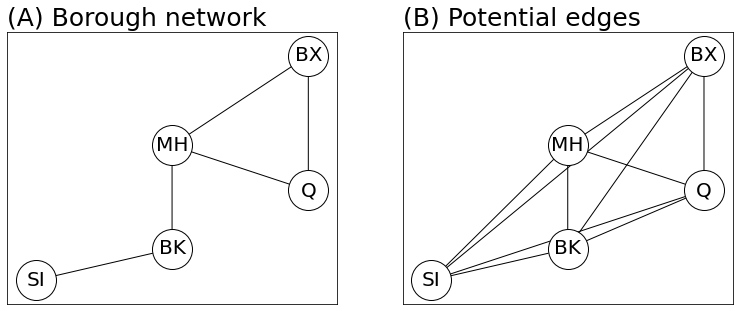
\includegraphics[width=0.8\linewidth]{representations/ch4/Images/density.png}
    \caption[Visualizing network density]{\textbf{(A)} The New York Borough network. The actual edges are shown. \textbf{(B)} The New York Borough network with all possible potential edges.}
    \label{fig:ch4:density}
\end{figure}

To put it all together, the \textit{network density} indicates the {density of edges} which are present in the network. For a simple network, the network density can be defined as the ratio between the total number of edges in $A$ and the total number of edges possible in $A$:
\begin{align}
    density(A) &= \frac{\sum_{j > i}a_{ij}}{\binom n 2} = \frac{2\sum_{j > i}a_{ij}}{n(n - 1)}
    \label{eqn:ch4:netdens}
\end{align}
In your example, this is simply the ratio of edges which {actually} exist to edges which could {possibly} exist, which is $\frac{5}{10} = 0.5$. You can compute the network density via \texttt{networkx} using the function \texttt{density()}:

\begin{lstlisting}[style=python]
nx.density(G)
# 0.5
\end{lstlisting}
In a simple network, there are a few additional ways you might see this equation written. Notice that the following inequality is true, by definition of a simple network:
\begin{align*}
    \sum_{i,j = 1}^n a_{ij} &= \sum_{j > i}a_{ij} + \sum_{i > j}a_{ij} + \sum_{i = 1}^n a_{ii} \\
    &= \sum_{j > i}a_{ij}+ \sum_{i > j}a_{ij} + 0,
\end{align*}
which is because the network is loopless (so the diagonal is $0$). Further, remember that $a_{ij} = a_{ji}$, which means that the first term is {exactly} equal to the second term, so:
\begin{align*}
    \sum_{i,j = 1}^n a_{ij} &= \sum_{j > i}a_{ij}+ \sum_{i > j}a_{ij} \\
    &= \sum_{j > i}a_{ij}+ \sum_{j > i}a_{ij} = 2\sum_{j > i}a_{ij} \\
    \Rightarrow \sum_{j > i}a_{ij} &= \frac{1}{2}\sum_{i,j = 1}^n a_{ij}
\end{align*}
This gives us the useful relationship that we can re-write the density even more simply, by plugging this relationship into Equation \eqref{eqn:ch4:netdens} as:
\begin{align*}
    density(A) &= \frac{\frac{1}{2}\sum_{i = 1}^n \sum_{j = 1}^n a_{ij}}{\binom n 2} = \frac{\sum_{i = 1}^n \sum_{j = 1}^n a_{ij}}{n(n - 1)}
\end{align*}
We wrote out the double sum here because there is a key relationship that we want to point out. Notice that the inner-most sum is just computing the degree $d_i$ of each node $i$, because $d_i = \sum_{j = 1}^n a_{ij}$ in an undirected network. This means that:
\begin{align}
    density(A) &= \frac{\frac{1}{2}\sum_{i = 1}^n d_i}{\binom n 2} = \frac{\sum_{i = 1}^n d_i}{n(n - 1)} \label{eqn:ch4:density_degree}
\end{align}
As a final note, notice that $\frac{1}{n}\sum_{i = 1}^n d_i$ is the \textit{average degree} over all of the $n$ nodes in the network. We will typically abbreviate this quantity using the symbol $d$. Using this fact with the right-most equality in Equation \eqref{eqn:ch4:density_degree}, we see that:
\begin{align*}
    density(A) &= \frac{d}{n - 1}.
\end{align*}
In this sense, the density can be conceptualized as the average degree of each node in the network, divided by the maximum possible degree each node could have (which, in a simple network, is $n-1$, since a node could at most have an edge to the other $n-1$ nodes in the network). This concept will become handy when we think about sparsity in Section \ref{sec:ch10:sparsity}.


\subsubsection{The clustering coefficient indicates how much nodes tend to cluster together}
\label{sec:ch4:prop-net:clustering}

The clustering coefficient indicates the fraction of triplets of nodes which are closed. What the heck is that? Let's look at only Brooklyn, Manhattan, Queens, and the Bronx, and temporarily ignore Staten Island:

\begin{lstlisting}[style=python]
G_clus = nx.Graph()

G_clus.add_node("MH", pos=(4,4))
G_clus.add_node("BK", pos=(4,1.7))
G_clus.add_node("Q", pos=(6,3))
G_clus.add_node("BX", pos=(6,6))


pos = nx.get_node_attributes(G, 'pos')
G_clus.add_edge("MH", "BX")
G_clus.add_edge("MH", "BK")
G_clus.add_edge("MH", "Q")
G_clus.add_edge("Q", "BX")

nx.draw_networkx(G_clus, with_labels=True, node_color="black", pos=pos,
                 font_color="white", edge_color="black")
\end{lstlisting}
The plotted result is shown in \ref{fig:ch4:subnet}(B).

To begin to define the clustering coefficient, you first must understand what a {triplet} is. A \textit{triplet} is an ordered tuple of three nodes which are connected by two or three edges. Note that a tuple of three nodes to be a triplet, you must be able to travel from one end of the triplet to the other along a contiguous path. The triplets are {closed} if there are three edges, and {open} if there are only two edges. For instance, in the above network, you have the following triplets of nodes:
\begin{enumerate}
    \item Open triplets between Bronx, Manhattan, and Brooklyn: (BX, MH, BK), (BK, MH, BX),
    \item Open triplets between Manhattan, Queens, and Brooklyn: (BK, MH, Q), (Q, MH, BK),
    \item Closed triplets between Bronx, Manhattan, and Queens: (BX, MH, Q), (BX, Q, MH), (MH, BX, Q), (MH, Q, BX), (Q, BX, MH), (Q, MH, BX),
\end{enumerate}

To clarify a fine technical point of open triplets, we do not count (BK, Q, MH) as a triplet because there is no edge from BK to Q. You must be able to go from the first node to the second to the third along edges that exist in the network in order for a triple of nodes to count as a triplet. No triplets are possible between Brooklyn, Bronx, and Queens, because only a single edge exists between the three of them. In your example, there are six closed triplets amongst the nodes (delineated in number 3. above), and there are 4 open triplets (delineated in numbers 1. and 2. above). The global clustering coefficient (or transitivity) is defined as:

\begin{align*}
    C &= \frac{\text{number of closed triplets}}{\text{number of closed triplets} + \text{number of open triplets}}
\end{align*}
In our example, this comes to $C = \frac{6}{6 + 4} = 0.6$. This equation can also be understood in terms of the adjacency matrix. Note that if a triplet between nodes $i$, $j$, and $k$ is closed, then all three of the potential edges $a_{ij}$, $a_{jk}$, and $a_{ki}$ have a value of $1$. Therefore, if you could the number of times that $a_{ij}a_{jk}a_{ki} = 1$, you also count the number of closed triplets! This means that the number of closed triplets can be expressed as $\sum_{i,j,k = 1}^na_{ij}a_{jk}a_{ki}$. 

Further, note that for a given node $i$, you can find an arbitrary triplet (either open or closed) through the following procedure.
1. Pick a single neighbor $j$ for node $i$. Note that the node $i$ has a number of neighbors equal to $degree(i) = d_i$, so there are $d_i$ possible neighbors to choose from.
2. Pick a different neighbor $k$ for node $i$. Note that since node $i$ had $d_i$ neighbors, it has $d_i - 1$ neighbors that are not node $j$.
3. Since you know that nodes $j$ and $k$ are both neighbors of node $i$, you know that $a_{ij}$ and $a_{ik}$ both have values of one, and therefore the edges $(i, j)$ and $(i, k)$ exist. Therefore, the tuple of nodes $(i, j, k)$ is a triplet, because {at least} two edges exist amongst the three nodes. This tuple is closed if the edge $(j, k)$ exists, and open if the edge $(j, k)$ does not exist.
4. Therefore, there are $d_i (d_i - 1)$ triplets in which node $i$ is the leading node of the triplet.

As it turns out, since triplets are {ordered tuples}, you can repeat this procedure for all nodes, and if you count how many triplets you get in total, you get the {total number of triplets} for the entire network. Therefore, the number of open and closed triplets in the network is the quantity $\sum_i d_i (d_i - 1)$.  Then you could express the clustering coefficient in terms of the adjacency matrix as:

\begin{align*}
    C &= \frac{\sum_{i,j,k = 1}^n a_{ij}a_{jk}a_{ki}}{\sum_{i = 1}^n d_i (d_i - 1)}
\end{align*}
Which gives you an expression to implement programmatically. You can compute the clustering coefficient via \texttt{networkx} using:

\begin{lstlisting}[style=python]
nx.transitivity(G_clus)
# 0.6
\end{lstlisting}


\subsubsection{The path length describes how far two nodes are}
\label{sec:ch4:prop-net:path}
How many bridges would you need to cross to get from Staten Island to Bronx? This concept relates directly to the concept of the {path length} in a network. A \textit{path} between two nodes $i$ and $j$ is a sequence of edges which starts at node $i$, and traverses through other nodes in the network until reaching node $j$. Two nodes are described as \textit{connected} if a path exists between them. The \textit{path length} is the number of edges in the path. For instance, if you remember your network from the New York example, you could get from Staten Island to Bronx in two possible ways, indicated in in (B) and (C) in Figure \ref{fig:ch4:path}.

\begin{figure}[h]
    \centering
    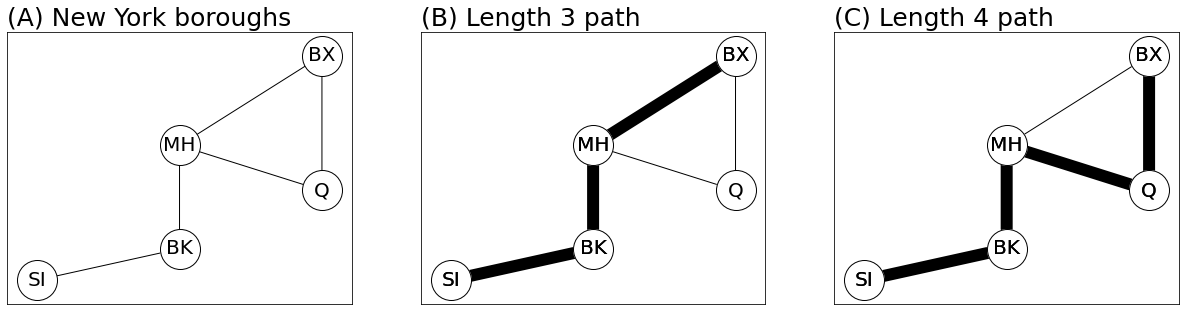
\includegraphics[width=\linewidth]{representations/ch4/Images/path.png}
    \caption[Path length in New York boroughs]{\textbf{(A)} The New York boroughs. \textbf{(B)} A length $3$ path from SI to BX. \textbf{(C)} A length $4$ path from SI to BX.}
    \label{fig:ch4:path}
\end{figure}
In this case, there are only two paths from SI to BX which do not visit the same node more than once, but in a larger network, there may be {many} possible paths from one node to another. For this reason, you will usually be interested in one particular path, the {shortest path}. The \textit{shortest path length} or \textit{distance} between nodes $i$ and $j$ is the path with the smallest path length that connects nodes $i$ and $j$. In your example, the shortest path is indicated by Figure \ref{fig:ch4:path}(B), and the shortest path length is therefore three.  If it is not possible to get from node $i$ to node $j$ using edges of the network, the shortest path length is defined to be infinite. The shortest path between nodes $i$ and $j$ will often be abbreviated using the notation $l_{ij}$.

A common statistic often calculated is the {distance matrix} for the network $L$, which is the $n \times n$ matrix whose entries $l_{ij}$ are the shortest path lengths between all pairs of nodes in the network. For your New York example, you can compute and visualize the distance matrix using:

\begin{lstlisting}[style=python]
L = nx.floyd_warshall_numpy(G)
heatmap(L, title="Distance matrix",  xticklabels=["SI", "MH", "BK", "Q", "BX"],
        yticklabels=["SI", "MH", "BK", "Q", "BX"], xtitle="Borough", ytitle="Borough")
\end{lstlisting}
Another common statistic you can compute using the distance matrix is the {average shortest path length}. The average shortest path length $l$ of a simple network is simply the average of all of the shortest paths between two distinct nodes $i$ and $j$ of the distance matrix:
\begin{align*}
    l &= \frac{1}{n(n - 1)}\sum_{i \neq j} l_{ij}
\end{align*}
The normalizing factor here is $n(n - 1)$ because the sum $\sum_{i \neq j}$ is short-hand for the double-sum $\sum_{i = 1}^n \sum_{j \neq i}$. Notice that the left-most sum has $n$ terms, and for each node $i$, there are $n-1$ other possible values that $j$ can take where $j \neq i$. This means that we are summing $n-1$ terms $n$ times (which is $n (n - 1)$). 

\paragraph{Paths in directed networks}

If the network is directed, the interpretation of a path is exactly the same, except you have to be careful to account for the directionality when finding paths from one node to the next. For instance, in Figure \ref{fig:ch4:directed}(B), there {is} a path from the nodes MH, Q, BX to SI or BK, but there are {no} paths from SI or BK to MH, Q, BX (as the bridge from BK to MH is out of service in the example).

\subsection{Subnetworks are subsets of larger networks}
\label{sec:ch4:prop-net:subnetwork}
When you think of an entire network, it is often useful to consider it in smaller bits. For instance, when you were looking at the clustering coefficient, you found it useful to break out the nodes {BK, Q, BX, MH} so you could count triplets, like we did in Section \ref{sec:ch4:prop-net:clustering}. 

This portion of the network is called a {subnetwork}. A \textit{subnetwork} is a network whose nodes and edges are {subsets} of the nodes and edges for another network. In this case, the  network toplogy of the New York example is $(\mathcal V, \mathcal E)$ defined by the sets:

\begin{enumerate}
    \item The nodes $V$: $\{SI, BK, Q, MH, BX\}$, and
    \item The edges $E$: $\left\{(SI, BK), (BK, MH), (MH, Q), (MH, BX), (Q, BX)\right\}$.
\end{enumerate}

and the subnetwork (which removed Staten Island, SI) we looked at above is the network:

\begin{enumerate}
    \item The nodes $V_s$: $\{BK, Q, MH, BX\}$, and
    \item The edges $E_s$: $\left\{(BK, MH), (MH, Q), (MH, BX), (Q, BX)\right\}$.
\end{enumerate}

As you can see, the subnetwork with nodes and edges $(V_s, E_s)$ is such that every element in $V_s$ is an element of $V$, and therefore the nodes of the subnetwork are a subset of the nodes of the complete network. Further, every element in $E_s$ is an element of $E$, and therefore the edges of the subnetwork are a subset of the edges of the complete network. So the subnetwork $(V_s, E_s)$ is a subnetwork of the network $(V, E)$. This particular subnetwork can be described further as an \textit{induced} subnetwork. A subnetwork of a network is \textit{induced} by a set of nodes if the following conditions hold:

\begin{enumerate}
    \item The nodes $V_s$ are a subset of the nodes of the network $V$, and
    \item The edges $E_s$ consist of {all} of the edges from the original network where both of the corresponding nodes are in $V_s$.
\end{enumerate} 

An example of the induced subnetwork we showed above is shown in Figure \ref{fig:ch4:subnet}(B). To see an example of a subnetwork which is {not} an induced subnetwork, check out Figure \ref{fig:ch4:subnet}(C). Try to determine why this subnetwork is not induced. You can create an induced subnetwork (in this case, by BK, MH, Q, BX) using networkx:

\begin{lstlisting}[style=python]
G_sg = G.subgraph(["BK", "MH", "Q", "BX"]).copy()
nx.draw_networkx(G_sg, with_labels=True, node_color="black", pos=pos,
                 font_color="white", edge_color="black")
\end{lstlisting}

\begin{figure}[h]
    \centering
    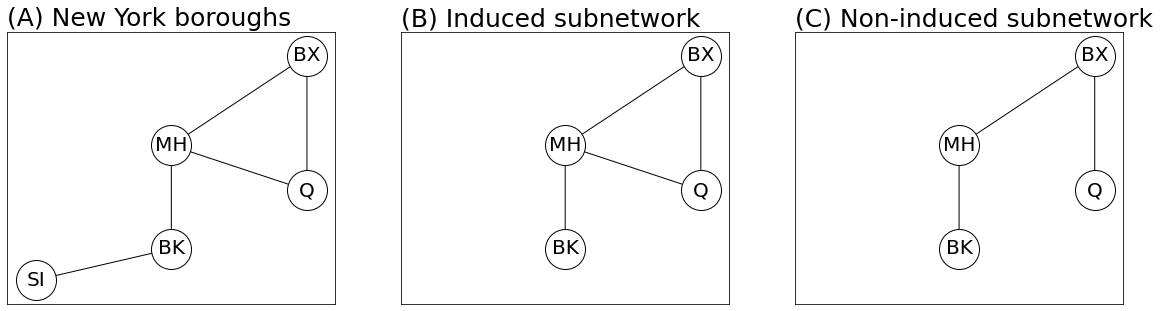
\includegraphics[width=\linewidth]{representations/ch4/Images/subnet.png}
    \caption[New York boroughs example]{\textbf{(A)} The New York Borough example. \textbf{(B)} The subnetwork induced by the node set \{BX, MH, Q, BX\}. This is also the example that we used to study clustering. \textbf{(C)} A subnetwork that is not an induced subnetwork.}
    \label{fig:ch4:subnet}
\end{figure}

\paragraph*{Representing subnetworks}
Notice that a subnetwork is a collection of nodes and edges defined on these nodes. Therefore, a subnetwork is itself also a network. This means that we could still represent a subnetwork using an adjacency matrix, with the caveat that the number of rows and columns might not be the same (since the nodes of a subnetwork are a subset of the nodes of the network) and the density might change (since the edges of a subnetwork are a subset of the edges of the network).

Let's think about why this matters.

\paragraph*{A caveat with the adjacency matrix of subnetworks}
Let's imagine that you have a simple network with the adjacency matrix $A$:
\begin{align*}
    A = \begin{bmatrix}
        0 & 0 & 0 \\
        0 & 0 & 1 \\
        0 & 1 & 0
    \end{bmatrix}
\end{align*}
And you consider a subnetwork that is induced by nodes \{2, 3\}. The induced subnetwork would have an adjacency matrix that looks like this:
\begin{align*}
    A_s = \begin{bmatrix}
        0 & 1 \\
        1 & 0
    \end{bmatrix}
\end{align*}
The key idea here is that, if you ignore the structure of the network when we do this, and conceptualize an induced subnetwork as a {deletion} of rows and columns, it becomes very difficult to figure out (later on in your analysis) which node is which. For instance, in your initial network, you might have also had a vector with $3$ elements (one for each node) that contained useful information about the nodes that you want to use later in your analysis. If you discard which nodes were included in your subnetwork, it will be very difficult (later in the analysis) to decipher which node is associated with which piece of information in your vector. For this reason, whenever you compute a subnetwork, we would {strongly} recommend that you make a note of it somewhere and store the nodes from the initial network that were retained in the subnetwork, so that you don't end up confused later on.

A particular induced subnetwork that you will often be concerned with is known as the largest connected component (LCC). 


\subsubsection{The largest connected component (LCC) is the largest subnetwork of connected nodes}
\label{sec:ch4:prop-net:lcc}
To define the largest connected component, we'll need to modify our example slightly. Let's say your network also includes the Boston area, and you have two new nodes, Boston (BO) and Cambridge (CA). Boston and Cambridge have several bridges between one another, so an edge exists between them. However, there are no bridges between boroughs of New York and the Boston area, so there are no edges from nodes in the Boston area to nodes in the New York area. Let's see how we would add this programmatically:

\begin{lstlisting}[style=python]
G_withbos = deepcopy(G)
G_withbos.add_node("BO", pos=(8, 6))
G_withbos.add_node("CA", pos=(8, 8))
G_withbos.add_edge("BO", "CA")
# fetch positions with boston and cambridge added
pos = nx.get_node_attributes(G_withbos, 'pos')
# plot
nx.draw_networkx(G_withbos, with_labels=True, node_color="black", pos=pos,
                font_color="white", edge_color="black")
\end{lstlisting}

We visualize the network with Boston and Cambridge in Figure \ref{fig:ch4:lcc}(A). 

The entire network can be described by the sets:
\begin{enumerate}
    \item $\mathcal V = \{SI, MH, BK, BX, Q, CA, BO\}$, and
    \item $\mathcal E = \{(SI, BK), (MH, BK), (MH, Q), (MH, BX), (MX, Q), (CA, BO)\}$.
\end{enumerate}

Notice that you have two distinct sets of nodes, those of New York and those of Boston, which are {only} connected amongst one another. Formally, these two sets of nodes can be described as inducing {connected components} of the network topology $(\mathcal V, \mathcal E)$. A \textit{connected component} is an induced subnetwork in which any two nodes are connected to each other by a path through the network. The two connected components are the New York induced subnetwork:

\begin{enumerate}
    \item The nodes $\mathcal V_N$: $\{SI, BK, Q, MH, BX\}$, and
    \item The edges $\mathcal E_N$: $\left\{(SI, BK), (BK, MH), (MH, Q), (MH, BX), (Q, BX)\right\}$.
\end{enumerate}

and the Boston induced subnetwork:
\begin{enumerate}
    \item The nodes $\mathcal V_B$: $\{CA, BO\}$, and
    \item The edges $\mathcal E_B$: $\left\{(CA, BO)\right\}$.
\end{enumerate}

We plot each individually in Figure \ref{fig:ch4:lcc}(B) and Figure \ref{fig:ch4:lcc}(C). If the network and the largest connected component are equivalent, we can omit the term {component}, and just say that the network is \textit{connected}.

\begin{figure}[h]
    \centering
    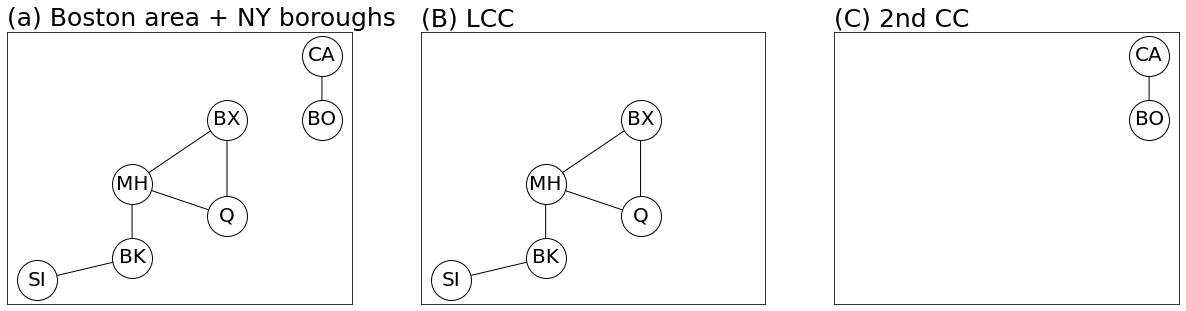
\includegraphics[width=\linewidth]{representations/ch4/Images/lcc.png}
    \caption[Connected Components]{\textbf{(A)} shows the New York boroughs with the added nodes for Boston and Cambridge. \textbf{(B)} shows the connected component induced by the boroughs of New York, which is also the LCC. \textbf{(C)} shows the connected component induced by Boston and Cambridge.}
    \label{fig:ch4:lcc}
\end{figure}
The \textit{largest connected component} (LCC) of a network is the connected component with the most nodes. In your example, the New York connected component has five nodes, whereas the Boston connected component has two nodes. Therefore, the New York connected component is the LCC of this simple network. You can compute the connected components and plot the largest connected component using \texttt{networkx} like this:

\begin{lstlisting}[style=python]
# returns a list of connected components, ordered 
# by decreasing size (#nodes)
cc_withbos = nx.connected_components(G_withbos)
# return the connected components, as networks
CC_nets = [G_withbos.subgraph(cc).copy() for cc in cc_withbos]

# plot the LCC
nx.draw_networkx(CC_nets[0], with_labels=True, node_color="black", pos=pos,
                font_color="white", edge_color="black")
\end{lstlisting}

A lot of times, when you are dealing with networks, they might already be in adjacency matrices. You can pass adjacency matrices directly into \texttt{graspologic} to obtain a LCC using:
\begin{lstlisting}
from graspologic.utils import largest_connected_component as lcc

A_withbos = nx.to_numpy_array(G_withbos)
A_lcc, retained_nodes = lcc(A_withbos, return_inds=True)
\end{lstlisting}
This is one of the {easiest} times for the caveat that we mentioned about subnetworks to arise. The \texttt{return\_inds} argument returns the rows/columns of \texttt{A\_withbos} that were retained for the LCC. The default functionality is to {not} return these indices, so proceed with caution!

\subsubsection{Connected components in directed networks}

The \textit{largest connected component} (LCC) of a network is the connected component with the most nodes. In your example, the New York connected component has five nodes, whereas the Boston connected component has two nodes. Therefore, the New York connected component is the LCC of this simple network.

Like the degree compared to the in- and out- degrees, for directed networks, connected components for directed networks need to be defined a little bit differently. A directed subnetwork is \textit{strongly connected} if directed paths exist between every pair of nodes in the subnetwork. 

A directed subnetwork is \textit{weakly connected} if the underlying directionalities are ignored, and the resulting undirected subnetwork is a connected component. Figure \ref{fig:ch4:directed}(C) shows an example of a strongly connected network, because you can travel along a path from each node to every other node in the network. On the other hand, Figure \ref{fig:ch4:directed}(B) shows an example of a weakly connected component when the bridge from MH to BK is out of service. This is because there is no longer a way to follow a path from SI or BK to MH, Q, and BX. When we ignore the arrows entirely, the resulting undirected network is still connected, as shown in Figure \ref{fig:ch4:directed}(A).


\newpage
\section{Types of network representations}
\label{sec:ch4:net-rep}

Now that you know how to represent networks with matrices and have some ideas of properties of networks, let's take a step back and take a look at what network representation is in general, and the different ways you might think about representing networks to understand different aspects of the network.

We already know that the topological structure of networks is just a collection of nodes, with pairs of nodes potentially linked together by edges. Mathematically, this means that a network is defined by two objects: the set of nodes, and the set of edges, with each edge just being defined as a pair of nodes for undirected networks. Networks can have additional structure: you might have extra information about each node (``features'' or ``covariates''), which we'll talk about when we cover Joint Representation Learning in Section \ref{ch6:joint}. Edges might also have weights, which are usually measure the connection strength in some way. We learned in the previous section that network topology can be represented with matrices in a number of ways -- with adjacency matrices, Laplacians, or (less commonly) with incidence matrices. 

One major challenge in working with networks is that a lot of standard mathematical operations and metrics remain undefined. What does it mean to add a network to another network, for instance? How would network multiplication work? How do you divide a network by the number 6? Without these kinds of basic operations and metrics, you are left in the dark when you try to find analogies to non-network data analysis.

Another major challenge has to do with the nature of network data. As it turns out, for any given number of nodes, there are a finite number of possible networks. When you have a finite number of possible outcomes, one of the most natural approaches is to attempt to use the data to try to describe each possible outcome individually. For instance, if you are flipping a coin, you might try to use the data (coin flips that you see) to determine with which probability the coin lands on heads or tails, since heads and tails are the two possible outcomes of the coin flip.

Unfortunately, we cannot possibly do this for network data. When a simple network has $n$ nodes, the number of possible networks that you could observe is $2^{\binom n 2}$ (we will derive this result later in Section \ref{sec:ch5:er}). We plot what this looks like in Figure \ref{fig:ch4:nnets}. When you allow for only 50 nodes, there are already more than $10^{350}$ possible networks. Just for reference, it is estimated that there are $10^{80}$ atoms in the known universe. If you created $10^{80}$ new universes, each with $10^{80}$ atoms, the total number of atoms across all universes would still be nowhere near this amount. 

In this section, we will explore the ways in which we conceptualize network representations to overcome this limitation. This section will prepare you to conceptualize the many particular strategies that you will learn later in Chapters \ref{sec:ch5} and \ref{sec:ch6}.

\begin{figure}[h]
    \centering
    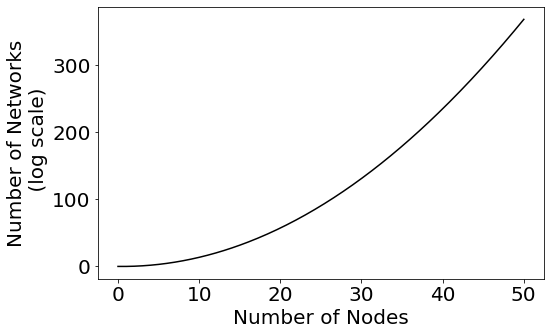
\includegraphics[width=0.7\linewidth]{representations/ch4/Images/nnets.png}
    \caption[Number of networks for $n$ nodes]{The number of possible distinct networks that you could have for a given number of nodes.}
    \label{fig:ch4:nnets}
\end{figure}

\subsection{Bag of Features}

The first approach is called the bag of features. The idea is that you take networks and you compute statistics from them, either for each node or for the entire network. These statistics could be simple things like the edge count or average path length between two nodes like you learned about in the last section, or more complicated metrics like the modularity {cite:p}`Newman2006Jun`, which measures how well a network can be separated into communities. Unfortunately, network statistics like these tend to be correlated; the value of one network statistic will almost always influence the other. This means that it can be difficult to interpret analysis that works by comparing network statistics. It's also hard to figure out which statistics to compute, since there are an infinite number of them.

\subsubsection{You Lose A Lot of Information with the Bag of Features Approach}

Let's take a look at a collection of networks in Figure \ref{fig:ch4:anascombe}:

\begin{figure}[h]
    \centering
    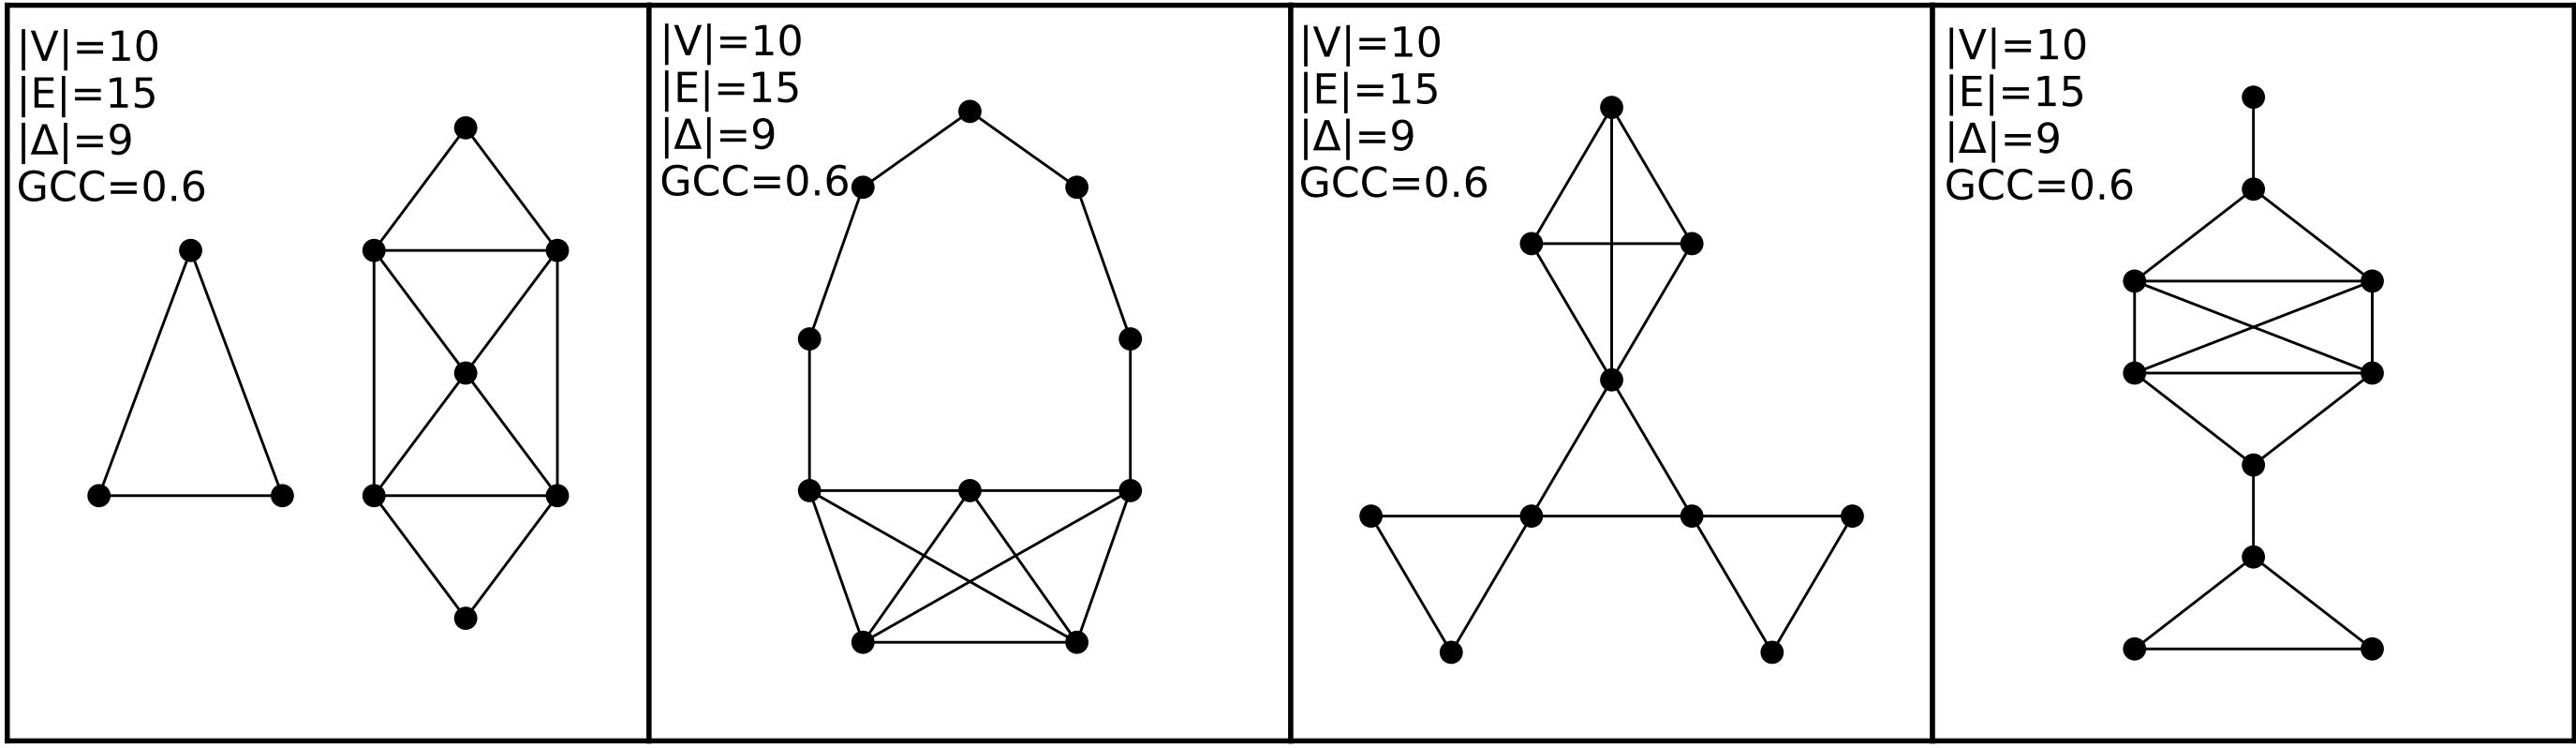
\includegraphics[width=\linewidth]{representations/ch4/Images/anascombe.jpeg}
    \caption[Very different networks can have the same summary statistics]{Four networks, all of which have the exact same network statistics for the four statistics we show here. They each have ten nodes and 15 edges. They also all contain the same number of closed triangles, and the same global clustering coefficient from Section \ref{sec:ch4:prop-net:clustering}.}
    \label{fig:ch4:anascombe}
\end{figure}

Each of these networks, however, are completely different from each other. The first network, for instance, has two connected components, while the others are all connected. The second network has a community of nodes that are only connected along a path, and a different community which are tightly connected, and so on. Modeling these networks through computing these features from them would lose a great deal of useful information about the topology of the network.


\paragraph{Network Features Tend to be Correlated}
\label{sec:ch4:net-rep:featurelims}

As we mentioned in the last paragraph, if you consider all possible networks, knowing the value of any of the network features gives you information about what the value of other network features might be.

Let's play around with this. We'll make $100$ random networks, each with $50$ nodes, and then we'll compute some common network statistics that people use in practice. Then, we'll look at how correlated these features are. For now, just think of a random network as being a network with each node being connected to each other node with some set probability. Each network will have a different connection probability. These networks will also have communities --- groups of nodes which have similar connection probabilities of being connected with other groups of nodes. 

Conceptually, you could think about a particular type of community structure using the bridge example that we covered previously when we talked about the Boston and New York boroughs in the LCC example in Section \ref{sec:ch4:prop-net:lcc}. It is probably more likely that two boroughs that are in the same state have a bridge between them then two boroughs in totally different states, right? When you generate data later on in this book, we'll get into different types of network models you can use. You don't need to have too good of an idea of what the below simulation code is doing just yet --- we will go into more depth in Chapter \ref{sec:ch5}.

\begin{lstlisting}[style=python]
from graspologic.simulations import sbm
import numpy as np
from numpy.random import uniform

n_nodes = 50
n_networks = 100
np.random.seed(1234)
# within-community probability
p = uniform(size=100, low=.5).round(2)
# between-community probability
q = uniform(size=100, high=.5).round(2)

networks = []
for i in range(n_networks):
    np.random.seed(1234)
    P = np.array([[p[i], q[i]],
                  [q[i], p[i]]])
    network = sbm(n=[n_nodes//2, n_nodes//2], p=P)
    networks.append(network)
\end{lstlisting}
Now, for each of these networks, we'll calculate a set of network features, using some of the various properties you learned about in the previous Section \ref{sec:ch4:prop-net}.

The only new statistic that we will look at is known as the network \textit{modularity}. You don't need to know too much about this statistic right now, other than the fact that it quantifies how much ``stronger'' the within-community effect is than the between-community effect (basically, that idea we described that New York boroughs would be more likely to have a bridge to other New York boroughs, than with either of the two cities in Massachusetts). The other statistics that we will compute will be the network density, the clustering coefficient, and the path length, all of which we discussed in Section \ref{sec:ch4:prop-net}.

The code below defines functions to calculate each of these network features, and then calculates them for each of the networks you created above.

We'll also define a preprocessing decorator, which just converts the network from a numpy array into the format networkx uses.


\begin{lstlisting}[style=python]
import functools
import networkx as nx

def preprocess(f):
    @functools.wraps(f)
    def wrapper(network):
        network = nx.from_numpy_matrix(network)
        return f(network)
    return wrapper

@preprocess
def modularity(network):
    communities = nx.algorithms.community.greedy_modularity_communities(network)
    Q = nx.algorithms.community.quality.modularity(network, communities)
    return Q

@preprocess
def network_density(network):
    return nx.density(network)

@preprocess
def clustering_coefficient(network):
    return nx.transitivity(network)

@preprocess
def path_length(network):
    if nx.number_connected_components(network) != 1:
        # You want to make sure this still works if your network isn't fully connected!
        network = max((network.subgraph(c) for c in nx.connected_components(network)), 
                      key=len)
    return nx.average_shortest_path_length(network)
\end{lstlisting}

Now, we'll calculate all of these features for each network, and finally we'll create a heatmap of their correlation.

\begin{lstlisting}[style=python]
import pandas as pd

network_features = []
for i, network in enumerate(networks):
    modularity_ = modularity(network)
    network_density_ = network_density(network)
    clustering_coefficient_ = clustering_coefficient(network)
    path_length_ = path_length(network)
    features = {"Modularity": modularity_, "Network Density": network_density_, 
                "Clustering Coefficient": clustering_coefficient_, "Average Path Length": path_length_}
    network_features.append(features)
    
df = pd.DataFrame(network_features)
feature_correlation = df.corr()
\end{lstlisting}
We show the results of this plot in Figure \ref{fig:ch4:anascombe}. Numbers close to 1 mean that when the first feature is large, the second tends to be large, numbers close to 0 mean that the features are not very correlated, and numbers close to -1 mean that when the first feature is large, the second feature tends to be small. 

\begin{figure}[h]
    \centering
    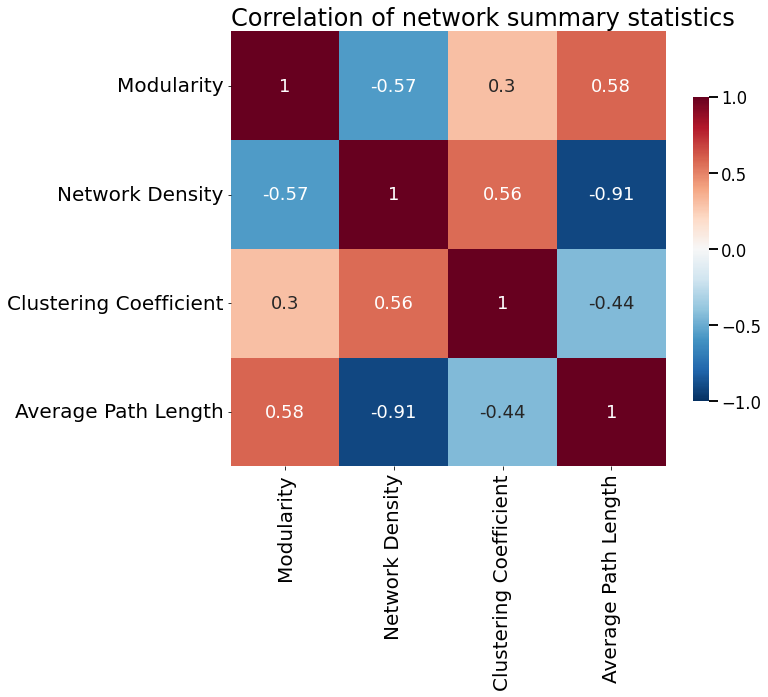
\includegraphics[width=0.8\linewidth]{representations/ch4/Images/corr.png}
    \caption[Correlation of netework features experiment]{The networks tend to exhibit correlation across various summary statistics. Note that none of the correlations are particularly close to $0$, and some (such as path length and density) are nearly perfectly correlated/anti-correlated.}
    \label{fig:ch4:corr}
\end{figure}

If you're familiar with correlation, that these numbers aren't particularly close to zero means that many of the features contain varying degrees of information about other features. Some of these features being big might say that another feature tends to also be high (positive correlation). Some of these features being big might say that another feature might tend to be the small (negative correlation). Some of these features don't tell you much about another particular feature (for instance, clustering and modularity only have a correlation with a magnitude around $0.3$), and some features are nearly perfectly informative about other features (network density and average path length are nearly perfectly negative-correlated with a value of $-.91$; that is, a high average path length implies a low network density, and vice versa). 

\paragraph{Why Network Feature Correlatedness Can Lead To Problems}

Let's take a step back to the implications of using the bag of features approach to analyze networks, now that you can see how correlated they usually are. Say you have a bunch of brain networks of mice, where the nodes are neurons and the edges are connections between neurons. You have a group of mice who were raised total darkness, and another group who were raised normally: let's call the ones who were raised in the darkness the batman mice. You're interested in how the visual parts of the brain are affected in the batman mice. You find the networks for only the visual parts of their brain, and then you calculate some network feature; maybe the density. It turns out that the network density is much lower for batman mice than it is for normal mice, so you conclude that raising mice in the darkness causes lower network density. Seems reasonable.

The problem is that network density is correlated with pretty much every other network feature you could have used. When you perform science, a primary focus of science tends to be establishing \textit{causality}. While we won't go much into causality here (there is an entire field dedicated to just this topic, called {causal inference}  for which there are many stellar reference texts), the jist is this. When you try to establish causality, you want to show a cause and effect type of relationship: the presence, or lack thereof, of some item $X$ {causes} an outcome $Y$ to happen. Whenever you do science, you want to find the root causes of {why} something is what it is: a mental illness is caused by a misfiring neuron, a misfolded protein is caused by the absence of a particular amino acid, a pair of friends having a major fight led to the students in a school being separated friendship wise into two distinct groups of people who support one student or the other. What you don't want to do is find something that just happens to be {correlated} with the thing that is impacted. 

For an example of this, we'll rotate back to our example from Section \ref{sec:ch1:howstudy:wontdiscuss}. If all smokers were older people and all non-smokers were younger people, just observing that the smokers tended to have higher rates of lung cancer would be insufficient to conclude whether smoking, or aging, cause lung cancer. Fortunately, statisticians found a way out: they took large groups of people with similar age ranges (and a number of other factors), and showed that the smokers had higher cancer rates (thus, ``untangling'' the correlatedness of age and smoking status). 

When you look at network features as things that potentially ``cause'' a particular effect, you can't really ``untangle'' the correlatedness of these network features, and it becomes extremely difficult, if not {impossible}  to actually establish which aspects of the network topology are actually causing or effected by the factor you are studying. 

For this reason, we think that network features are useful to {ascertain} whether something has an effect on the network, and provide information as to which directions you might want to look to establish causality. However, network features alone are insufficient, in our opinion, for defining causality. 

\subsection{Bag of Edges}
\label{sec:ch4:net-rep:bagofedges}

The second approach to studying networks is called the bag of edges. Here, you just take all of the edges in your network and treat them all as independent entities. You study each edge individually, ignoring any interactions between edges. This can work in some situations, but you still run into dependence: if two people within a friend group are friends, that can change the dynamic of the friend group and so change the chance that a different set of two people within the group are friends.

More specifically, in the bag of edges approach, you generally assume that every edge in your network will exist with some particular {probability} which can be different depending on the edge that you're looking at. For example, there might be a 60\% chance that the first and second nodes in your network are connected, but only a 20\% chance that the third and fourth nodes are. What often will happen here is that you have multiple networks describing the same (or similar) systems. For example, let's use the mouse example again from above. You have your batman mice (who were raised in the dark) and your normal mice. You'll have a network for each batman mouse and a network for each normal mouse, and you assume that, even though there's a bit of variation in what you actually see, the {probability} of an edge existing between the same two nodes is the same for all batman mice. Your goal would be to figure out which edges have a different {probability} of existing with the batman mice compared to the normal mice.

Let's make some example networks to explore this. We'll have two groups of networks, and all of the networks will have only three nodes for simplicity's sake. Each group will contain 20 networks, for a total of 40 networks. In the first group, every edge between every pair of nodes simply has a 50\% chance of existing. In the second group, the edge between nodes 0 and 1 will instead have a 90\% chance of existing, but every other edge will still just be 50\%. We'll generate ten networks from the first group, and ten networks from the second group.

\begin{lstlisting}[style=python]
from graspologic.simulations import sample_edges

P1 = np.array([[.5, .5, .5],
               [.5, .5, .5],
               [.5, .5, .5]])

P2 = np.array([[.5, .9, .5],
               [.9, .5, .5],
               [.5, .5, .5]])

# First group
n_networks = 20
networks = np.empty((2*n_networks, 3, 3))
for i in range(n_networks):
    networks[i,:,:] = sample_edges(P1)

# Second group
for i in range(n_networks, 2*n_networks):
    networks[i,:,:] = sample_edges(P2)

ys = np.array([1 for i in range(0, n_networks)] + [2 for i in range(0, n_networks)])
\end{lstlisting}

\subsubsection{Figuring out which edge is the signal edge}

By design, you know that the edge between nodes 0 and 1 has signal - the probability that it's there changes depending on whether your network is in the first or the second group. One common goal when using the bag of edges approach is finding signal edges: edges whose probability of existing changes depending on which type of network you're looking at. In your case, we're trying to figure out (without using your prior knowledge) that the edge between nodes 0 and 1 is a signal edge.

To find the outlier edge, you'll first get the set of all edges, along with their indices. Since all of your networks are undirected, you'll get the edges and their indices by finding all of the values in the the upper-triangular portion of the adjacency matrices.

\begin{lstlisting}[style=python]
edge_indices = np.triu_indices(3, k=1)
\end{lstlisting}

Now, you'll use a hypothesis test called the {Fisher's Exact Test} to find the outlier edge. You don't need to worry too much about what fisher's exact test is; here it is just something that will let us quantify whether an edge is different between the two groups, while makes limited assumptions about your data. We'll talk more about it in Section \ref{sec:ch9:ssn_incoherent}. 

In the code below, we:
\begin{enumerate}
    \item Loop through the edge indices,
    \item Get a list of all instances of that edge in the first group, and all instances of that edge in the second group, and
    \item Feed that list into the Fisher's exact test and obtain $p$-values (small $p$-value = more signal).
\end{enumerate}

\begin{lstlisting}[style=python]
from scipy.stats import fisher_exact

edge_pvals = []
for i, j in zip(*edge_indices):
    gr1_edge = networks[ys == 1,i,j].sum()  # number of group1 with edge i,j
    gr2_edge = networks[ys == 2,i,j].sum()  # number of group2 with edge i,j
    gr1_noedge = n_networks - gr1_edge  # number of group1 without edge i,j
    gr2_noedge = n_networks - gr2_edge  # number of group2 without edge i,j
    
    edge_tab = np.array([[gr1_edge, gr2_edge], [gr1_noedge, gr2_noedge]])  # arrange as in table
    
    edge_pvals.append(fisher_exact(edge_tab).pvalue)
\end{lstlisting}
You can see below that the $p$-value for the first edge, the one that connects nodes 0 and 1, is extremely small, whereas the $p$-values for the other two edges are relatively large.

\begin{lstlisting}[style=python]
np.array(edge_pvals).round(3)
\end{lstlisting}

\subsection{Bag of Nodes}
\label{sec:ch4:net-rep:bagofnodes}

Similarly to the bag of edges, you can treat all of the nodes as their own entity and do analysis on a bag of nodes. Much of this book will focus on the bag of nodes approach, because we'll often use edge count, covariate information, and other things when we work with bags of nodes. Although there's still correlation between nodes, it generally isn't as big of an issue. Most of the single-network methods you'll use in this book will take the bag of nodes approach. 

What we'll see repeatedly is that we take the nodes of a network and {embed} them so each node is associated with a point on a plot (this is called the {node latent space}). In a sense, this will ``tabularize'' our data, which as we learned in Section \ref{sec:ch1:challenges}, overcomes a major hurdle of network machine learning. Then, we can use other methods from mainstream machine learning to learn about our network. Deciding how to handle these ``bags of nodes'' will be a prime focus of Chapter \ref{sec:ch6}, and we will devote attention in Part \ref{p:app} to determining how we can use these bags of nodes.

We'll also often associate node representation with community investigation. The idea is that sometimes you have groups of nodes which behave similarly -- maybe they have a higher chance of being connected to each other, or maybe they're all connected to certain other groups of nodes. Regardless of how you define communities, a community investigation motif will pop up: you get your node representation, then you associate nearby nodes to the same community. We can then look at the properties of the node belonging to a particular community, or look at relationships between communities of nodes.

Since we'll use the bag of nodes approach heavily throughout this book, you'll be getting a much better sense for what you can do with it later. As a sneak preview right now, let's generate a few networks and embed their nodes to get a feel for what bag-of-nodes type analysis might look like. 

Don't worry about the specifics, but below you generate a simple network with two communities. Nodes in the same community have an 80\% chance of being connected, whereas nodes in separate communities have a 20\% chance of being connected. This is like saying that boroughs of New York \textit{or} boroughs near Boston have an 80\% of being connected by bridges, but boroughs of New York and boroughs near Boston have a 20\% chance of having a bridge between them. There are 20 nodes per community. Again, we'll cover the intuition of this particular generative model a lot more in Chapter \ref{sec:ch5}, so keep the big picture in focus for now.

\begin{lstlisting}[style=python]
from graspologic.simulations import sbm

# generate network
P = np.array([[.8, .2,],
              [.2, .8]])
network, labels = sbm(p=P, n=[20, 20], return_labels=True)
\end{lstlisting}

Now, you'll use graspologic to find the points in 2D space that each node is associated with. Again, don't worry about the specifics: this will be heavily explained later in the book. All you have to know right now is that we're {mapping} (transforming) the nodes of your network from network space, where each node is associated with a set of edges with other nodes, to the a tabular space, where each node is associated with an $x$-coordinate and a $y$-coordinate.

\begin{lstlisting}[style=python]
from graspologic.embed import AdjacencySpectralEmbed as ASE

ase = ASE(n_components=2)
embedding = ase.fit_transform(network)
\end{lstlisting}

Figure \ref{fig:ch4:bagonode} shows the result of this tabularization by community. Each of the dots in this plot is one of the nodes of your network. You can see that the nodes cluster into two groups: one group for the first community, and another group for the second community. Using this representation for the nodes of your network, you can open the door to later downstream machine learning tasks.

\begin{lstlisting}[style=python]
from graphbook_code import plot_latents, draw_cartesian, add_circle, text

ax = draw_cartesian(xrange=(-1, 1), yrange=(-1, 1))
plot = plot_latents(embedding, labels=labels, ax=ax)
plot.set_title("Bag of Nodes on a coordinate axis", y=1.1);

# plot circle
x_centroid, y_centroid = embedding[labels==0].mean(axis=0)
add_circle(x_centroid, y_centroid+.2, ax=ax)
ax.annotate("Nodes plotted \nas 2d points", xy=(x_centroid-.2, y_centroid+.2), xytext=(x_centroid-2, y_centroid), 
            arrowprops={"arrowstyle": "->"});
\end{lstlisting}
\begin{figure}[h]
    \centering
    \includegraphics[width=\linewidth]{representations/ch4/Images/bagonode.png}
    \caption{Nodes in the same community ending up being in similar areas of the $x$/$y$ coordinate axis above.}
    \label{fig:bagonode}
\end{figure}

\subsection{Bag of Networks}
\label{sec:ch4:net-rep:bagofnets}

The last approach is the bag of networks, which you'd use when you have more than one network that you're working with. Here, you'd study the networks as a whole and you'd want to test for differences across different networks or classify entire networks into one category or another. You might want to figure out the groups of networks look different, or whether you can learn information across all of the networks simultaneously. This is can be useful if you have many extremely large networks, with millions of nodes.

To showcase the bag of networks approach, let's create a few networks. We'll have one group of networks distributed the same way, and another group distributed differently. What you want to do is plot each network as a point in space, so that you can see the communities of networks directly.

Both sets of networks will have two communities of nodes, but the first set will have slightly stronger within-community connections than the second. Each network will have 200 nodes in it, 100 for each community.

\begin{lstlisting}[style=python]
def make_network(*probs, n=100, return_labels=False):
    pa, pb, pc, pd = probs
    P = np.array([[pa, pb], 
                  [pc, pd]])
    
    return sbm([n, n], P, return_labels=return_labels)

n = 100
p1, p2, p3 = .12, .06, .03

first_group = []
for _ in range(6):
    network = make_network(p1, p3, p3, p1)
    first_group.append(network)
    
second_group = []
for _ in range(12):
    network = make_network(p2, p3, p3, p2)
    second_group.append(network)
\end{lstlisting}

\begin{lstlisting}[style=python]
\end{lstlisting}
Again, don't worry too much yet about the process with which these networks were generated - that will all be explained in the next chapter. All you need to get out of this code is that you have six networks from the first group, and another twelve networks from the second. You can see these networks in heatmap form below. These networks are plotted in Figure \ref{fig:ch4:bagonets}(A). 

Now, you have to figure out some way of plotting each network as a point in space. Here's a rough overview for how you'll do it.

First, you'll take all of your networks and find a common space that you can orient all of the nodes into. The nodes for all of the networks will exist in the same space, meaning their locations can be compared with each other. We'll have a bunch of matrices, one for each network. Since each network has 200 nodes, and we're embedding into 2-dimensional space, we'll have six 200 by 200 matrices for the first group of networks, and another twelve 200 by 200 matrices for the second group. This process is called finding a {network} latent space with a homogeneous {node latent space}  and will be extremely valuable for embedding collections of networks later on. Again, this takes our collection of networks and \textit{tabularizes} them for us, taking each $200 \times 200$ adjacency matrix and turning it into a $200 \times 2$ matrix, effectively ``bagging the nodes'' like we did in the preceding section.

Next, once we have a bag of nodes for each network, we can use standard machine learning techniques with them. Here, we'll use classical multi-dimensional scaling (MDS), a popular dimensionality reduction technique. We'll do this by constructing a dissimilarity matrix which captures how dissimilar each ``bag of nodes'' is between every pair of networks, and then embed this dissimilarity matrix. This second embedding, in effect, tabularizes each network individually and gives us a bag of networks representation.

Again, don't worry if you don't understand the details: embedding and how it works will be explained in future chapters.

\begin{lstlisting}[style=python]
from graspologic.embed import OmnibusEmbed as OMNI
from graspologic.embed import ClassicalMDS

# Find a node latent space for the nodes of all of your networks
omni = OMNI(n_components=2)
omni_embedding = omni.fit_transform(first_group + second_group)

# embed each network representation into a 2-dimensional space
cmds = ClassicalMDS(2)
cmds_embedding = cmds.fit_transform(omni_embedding)

# Find and normalize the dissimilarity matrix
distance_matrix = cmds.dissimilarity_matrix_ / np.max(cmds.dissimilarity_matrix_)
\end{lstlisting}

You can see the dissimilarity matrix in Figure \ref{fig:ch4:bagonets}(B). As you can see, there look to be two groups of networks that tend to be quite similar amongst themselves, and quite different between the groups. The diagonals of the matrix are all 0, because the dissimilarity between a network and itself is 0.

Embedding this {new} matrix will give us a point in space for each network. Once you find the embedding for this dissimilarity matrix via MDS as above, you can plot each of the networks in space. Since there are six networks of the first type and twelve of the second type, one of the clusters has six dots, and the other has twelve dots. Let's take a look at this plot:
\begin{lstlisting}[style=python]
ax = draw_cartesian(xrange=(-1, 1), yrange=(-1, 1))
plot_latents(cmds_embedding, ax=ax, labels=labels)
\end{lstlisting}

\begin{figure}
    \centering
    \includegraphics[width=\linewidth]{representations/ch4/Images/bagonets.png}
    \caption[Bags of networks]{\textbf{(A)} the networks from each of the two groups. \textbf{(B)} The dissimilarity matrix between pairs of networks. \textbf{(C)} Each point represents a single network point in space. We can easily see the two clusters, which represent the two types of networks you created.}
    \label{fig:ch4:bagonets}
\end{figure}

\newpage
\section{Regularization}
\label{sec:ch4:regularization}

In practice, many networks you will encounter in network machine learning will not be simple networks: Many of the techniques we discuss will be just fine to use with weighted networks. Unfortunately, real world networks are often extremely noisy, and so the analysis of one real world network might not generalize very well to a similar real world network. For this reason, we turn to regularization. 

\textit{Regularization} is the process by which you either:
\begin{enumerate}
    \item Modify data for the purpose of mitigating overfitting due to idiosyncrasies of the observed data, and/or
    \item Modify the function you are estimating due to its fragility to the idiosyncracies of the observed data.
\end{enumerate}

In network machine learning, the first step of your analysis is to typically modify the network (or networks) themselves to allow better generalization of your statistical inference to new datasets. Later chapters will cover approaches in which you modify the function you are estimating.

For each of the following subsections, we'll pose an example, a simulation, and code for how to implement the desired regularization approach. It is important to realize that you might use several of these techniques simultaneously in practice, or you might have a reason to use these techniques that go outside of our working examples.

We start with a few running examples for this section. We have two non-simple networks:

\begin{floatingbox}[h]\caption{Activity/hobby network}
The nodes of this network are a group of $50$ area students, the first $25$ of whom are athletes, and the second $25$ are in marching band. To collect the first network, you ask each student to select from a list of $50$ school activities and outside hobbies that they enjoy. For a pair of students $i$ and $j$, the weight of their interest alignment will be a score between $0$ and $50$ indicating how many activities or hobbies that they have in common. 

We will refer to this network as the activity/hobby network. This network is undirected, since if student $i$ shares $x$ activities or hobbies with student $j$, then student $j$ also shares $x$ activities or hobbies with student $i$. This network is weighted, since the score is between $0$ and $50$. Finally, this network is loopless, because it would not make sense to look at the activity/hobby alignment of a student with themself, since every student would have perfect alignment of activities and hobbies with him or herself. 

Because the network is undirected, the researchers have only saved half the portion of the adjacency matrix that includes the entries $a_{ij}$ where $j > i$.
\end{floatingbox}

\begin{floatingbox}[h]\caption{Friendship network}
This network is collected using the same $50$ students as the activity/hobby network. To collect the second network, you ask each student to rate how good of friends they are with other students, on a scale from $0$ to $1$. A score of $0$ means they are not friends with the student or do not know the student, and a score of $1$ means the student is their best friend. We will refer to this network as the friendship network. This network is directed, since two students may differ on their understanding of how good of friends they are. This network is weighted, since the score is between $0$ and $1$. Finally, this network is also loopless, because it would not make sense to ask somebody how good of friends they are with themself.
\end{floatingbox}

Our scientific question of interest is how well activities and hobbies align with perceived notions of friendship. You want to use the networks of Examples 3.3 and 3.4 to learn about a hypothetical third network, whose nodes are identical to these two networks, but whose edges are whether the two individuals are friends (or not) on facebook. To answer this question, you have to do to some work to make your networks better suited to the task! We'll simulate some example networks, with output in Figure \ref{fig:ch4:friendex}.

\begin{lstlisting}[style=python]
from graspologic.simulations import sbm
import numpy as np

wtargsa = [[dict(n=50, p=.09), dict(n=50, p=.02)],
          [dict(n=50, p=.02), dict(n=50, p=.06)]]

wtargsf = [[dict(a=4, b=2), dict(a=2, b=5)],
          [dict(a=2, b=5), dict(a=6, b=2)]]

# activity network as upper triangle matrix
A_activity_uppertri = sbm(n=[25, 25], p=[[1,1], [1,1]], wt=np.random.binomial, wtargs=wtargsa, loops=False, directed=False)
A_activity_uppertri = np.triu(A_activity_uppertri)

# friend network
A_friend = sbm(n=[25, 25], p=[[.8, .4], [.4, 1]], wt=np.random.beta, wtargs=wtargsf, directed=True)
\end{lstlisting}

\begin{figure}[h]
    \centering
    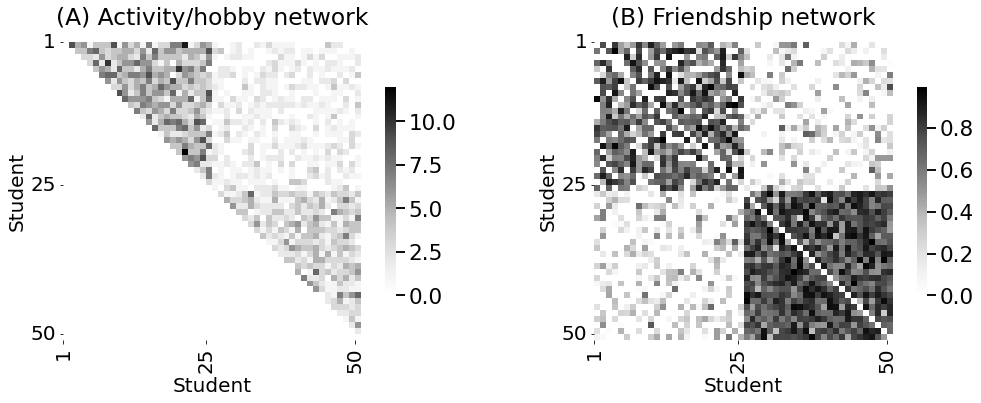
\includegraphics[width=\linewidth]{representations/ch4/Images/friendex.png}
    \caption[Friendship and activities networks]{A comparison of the two networks that we sampled to use in this section. The friendship network is shown in \textbf{(A)}, and the activity/hobby network is shown in \textbf{(B)}.}
    \label{fig:ch4:friendex}
\end{figure}

%% ALEX STOPPING POINT 07/02 4:36pm}

We'll also work with a third network which will have unique particularities from the preceding two, where we want to ask a question about only this network itself. 
\begin{floatingbox}[h]\caption{Unrelated business network}
The $17$ nodes in the network are local businesses, and an edge exists between a pair of businesses if they have business dealings with one another (they buy or sell products from/with the company). Three of these businesses operate in total exclusion and do not have any edges. Three of these businesses only work with one other business. One businesses work with all of the non-excluded businesses. 
\end{floatingbox}

To begin, we're going to start looking at the business network. Let's take a look at what this network looks like in Figure \ref{fig:ch4:businessex}.

\begin{lstlisting}[style=python]
from graphbook_code import heatmap
from matplotlib import pyplot as plt
from graspologic.simulations import er_np
import networkx as nx

n = 10
A_bus = er_np(n, 0.6)

# add pendants
n_pend = 3
A_bus = np.column_stack([np.row_stack([A_bus, np.zeros((n_pend, n))]), 
                         np.zeros((n + n_pend, n_pend))])

n = n + n_pend
# add pizza hut node
n_pizza = 1
A_bus = np.column_stack([np.row_stack([A_bus, np.ones((n_pizza, n))]), 
                         np.ones((n + n_pizza, n_pizza))])
n = n + n_pizza

# add isolates
n_iso = 3
A_bus = np.column_stack([np.row_stack([A_bus, np.zeros((n_iso, n))]), 
                         np.zeros((n + n_iso, n_iso))])
A_bus = A_bus - np.diag(np.diag(A_bus))
n = n + n_iso

# as a heatmap
node_names = [i for i in range(0, n)]
heatmap(A_bus.astype(int), title="Business Network Adjacency Matrix", 
               xticklabels=node_names, yticklabels=node_names)
# as a layout plot
G_bus = nx.from_numpy_matrix(A_bus)
node_pos = nx.shell_layout(G_bus)

plt.figure()
nx.draw(G_bus, pos=node_pos)
\end{lstlisting}

\begin{figure}[h]
    \centering
    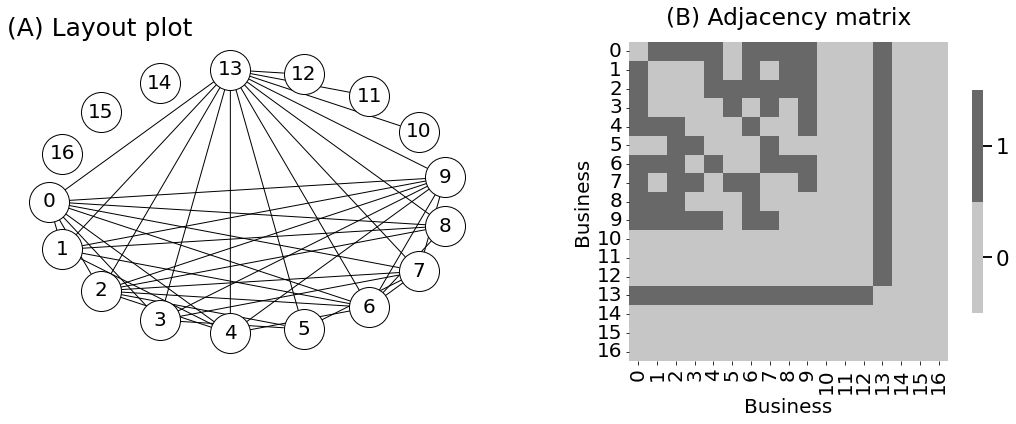
\includegraphics[width=\linewidth]{representations/ch4/Images/businessex.png}
    \caption[Business network example]{An example of a business network, where nodes are businesses and edges are whether the pairs of businesses have a business relationship.}
    \label{fig:ch4:businessex}
\end{figure}

\subsection{Node pruning}

Node pruning is a regularization technique in which you remove nodes for one reason or another. Typically, you will remove nodes due to some property about their degrees, or other properties (such as their \emph{connectedness} with other nodes that you care about). These strategies are covered loosely in the book \cite{Barabsi2013Mar}, and can be found in more computation-heavy network papers. Let's take a look at some of the strategies.

\subsubsection{Degree trimming removes nodes with unfavorable degrees}

In your business network, there are several nodes which tend to impart ``strange'' properties on downstream machine learning tasks. Some of these nodes, which include nodes with disproportionately high or low values, tend to yield numerical instability when you apply machine learning algorithms to them. By ``numerical instability'', what we mean is that the the (few) connections that nodes with low degrees have are going to have a disproportionately large impact on the machine learning task we perform. For this reason, it may be advantageous to remove nodes whose degrees are much different from the other nodes in the network. 

One special case of degree trimming is called removing \emph{isolates}. An \textit{isolated node} is a node which has a degree of $0$, meaning that it is not connected to any other nodes in the network. See if you can spot the isolates in Figure \ref{fig:ch4:businessex}.

Another special case of degree trimming is called the removal of \emph{pendants}. A \textit{pendant node} is a node which has a degree of $1$, meaning that it is only connected to one other node in the network. Try and see if you can spot the pendants in \ref{fig:ch4:businessex}.

You can remove isolates or pendants pretty simply. You simply need to compute the degree of each node in the network, and then retain the nodes with a degree \emph{above} your chosen threshold. To remove isolates, you would pick this threshold to be $0$ (retain nodes with non-zero degree), and to remove both pendants and isolates, you would pick this threshold to be $1$ (retain nodes with a degree exceeding $1$). You can do this like follows:
\begin{lstlisting}[style=python]
def compute_degrees(A):
    # compute the degrees of the network A
    # since A is undirected, you can just sum
    # along an axis.
    return A.sum(axis=1)

def prune_low_degree(A, return_inds=True, threshold=1):
    # remove nodes which have a degree under a given
    # threshold. For a simple network, threshold=0 removes isolates,
    # and threshold=1 removes pendants
    degrees = compute_degrees(A)
    non_prunes = degrees > threshold
    robj = A[np.where(non_prunes)[0],:][:,np.where(non_prunes)[0]]
    if return_inds:
        robj = (robj, np.where(non_prunes)[0])
    return robj

A_bus_lowpruned, nonpruned_nodes = prune_low_degree(A_bus)
\end{lstlisting}

Next, we'll plot the network as a layout plot. Remember how we told you in Section \ref{sec:ch4:prop-net:subnetwork} that if you just ``threw away'' nodes ignorant of which ones you threw away that you would run into trouble? Here's a good example of that. If you had just pruned the low degree nodes, you would have no idea which nodes were originally plotted \emph{where} in the initial layout plot that you looked at. Fortunately, since we included this information, we can recover the spatial position of each node pretty easily, and replot the network with the nodes that were not pruned in the same place that they were before:

\begin{lstlisting}[style=python]
node_names_lowpruned = [node_names[i] for i in nonpruned_nodes]
node_pos_lowpruned = {i : node_pos[j] for i, j in enumerate(nonpruned_nodes)}

G_bus_lowpruned = nx.from_numpy_matrix(A_bus_lowpruned)

nx.draw(G_bus_lowpruned, pos=node_pos_lowpruned)
\end{lstlisting}

The resulting layout plot is shown in Figure \ref{fig:ch4:nodeprune}(A).

\begin{figure}[h]
    \centering
    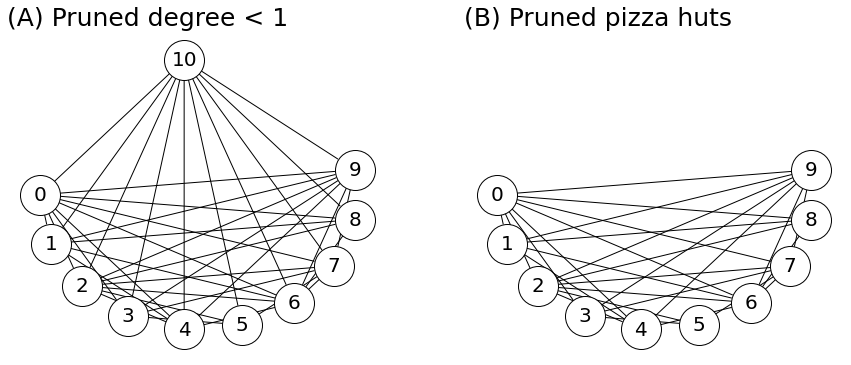
\includegraphics[width=\linewidth]{representations/ch4/Images/nodeprune.png}
    \caption[Pruning high and low degree nodes]{\textbf{(A)} The business network after pruning nodes with a degree less-than or equal to $1$, which consists of isolates and pendants. \textbf{(B)} The business network after pruning isolates and pendants followed by pizza-hut nodes.}
    \label{fig:ch4:nodeprune}
\end{figure}

A useful way to determine whether you have isolates or pendants is to look at the \emph{degree distribution histogram} of the network. The degree distribution histogram just shows a y axis of counts for a given range of possible x values. When the values you want a histogram for can only take a limited number of possible values, you might be able to get away with just looking at each possible value as its own x-axis point. Sometimes, when the values can take a large number of possible values, this might not be possible. You might have to \emph{bin} similar values together to make the plot appreciable. The degree distribution, before and after removing pendants/isolates, looks like this:

\begin{lstlisting}[style=python]
degrees_before = compute_degrees(A_bus)
degrees_after = compute_degrees(A_bus_lowpruned)
\end{lstlisting}

and can be plotted like this:

\begin{lstlisting}[style=python]
from seaborn import histplot
fig, axs = plt.subplots(1,2, figsize=(15, 4))

ax = histplot(degrees_before, ax=axs[0], binwidth=1, binrange=(0, 14))
ax.set_xlabel("Node degree");
ax.set_ylabel("Number of Nodes");
ax.set_title("Business Network, before pruning");
ax = histplot(degrees_after, ax=axs[1], binwidth=1, binrange=(0, 14))
ax.set_xlabel("Node degree");
ax.set_title("Business Network, after pruning")
\end{lstlisting}

\paragraph{Removing pizza hut nodes}

On the other end of the spectrum, it is often useful to remove nodes which don't really tell us anything about the network at all because they are just connected to \emph{everything}. We call these nodes \emph{pizza hut} nodes, because let's face it, pizza hut can be delivered pretty much anywhere! After pruning, we actually \emph{created} a pizza hut node, which you can see from low-degree pruned network in Figure \ref{fig:ch4:nodeprune}(A). 

We can prune these nodes just as easily as before. This time, note that our pruning threshold is simply set as the maximum possible node degree. Further, note that since we pruned the pizza-hut node from the low-pruned network, we need to recover which nodes from the original network were retained. This should further emphasize to you the importance of keeping track of your indices whenever you remove nodes from your network, as you can imagine that if you do a lot of node prunings, this can get confusing rapidly:

\begin{lstlisting}[style=python]
def prune_high_degree(A, return_inds=True, threshold=0):
    # remove nodes which have a degree over a given
    # threshold. For a simple network, threshold=A.shape[0] - 1
    # removes any pizza hut node
    degrees = compute_degrees(A)
    non_prunes = degrees < threshold
    robj = A[np.where(non_prunes)[0],:][:,np.where(non_prunes)[0]]
    if return_inds:
        robj = (robj, np.where(non_prunes)[0])
    return robj

# pruning nodes 
A_bus_pruned, highpruned_nodes = prune_high_degree(A_bus_lowpruned, threshold=A_bus_lowpruned.shape[0] - 1)

# get the nodes that aren't pruned by low pruning nor pizza hut node pruning
node_names_pruned = [node_names_lowpruned[i] for i in highpruned_nodes]
node_pos_pruned = {i : node_pos_lowpruned[j] for i, j in enumerate(highpruned_nodes)}

G_bus_retained = nx.from_numpy_matrix(A_bus_pruned)
nx.draw(G_bus_retained, pos=node_pos_pruned)
\end{lstlisting}
The result of both low-degree pruning (for isolates and pendants) and high-degree pruning (for pizza hut nodes) is shown in Figure \ref{fig:ch4:nodeprune}(B). 

Again, you might want to visualize the degree distribution plot to decide whether you want to prune nodes with high degrees.

\subsubsection{The Largest Connected Component is the largest subnetwork of connected nodes}

Two sections ago in Section \ref{sec:ch4:prop-net:lcc}, you learned about computing the largest connected component. This is a node pruning technique, because it "throws out" all of the nodes other than the ones which are in the largest connected component. We would encourage you to go back through this example now if you have time, so that you will better associate it as a regularization technique in your brain.


\subsection{Regularizing the edges of unweighted networks}

\subsubsection{Symmetrizing the adjacency matrix gives us undirectedness}
\label{sec:ch4:regularization:symmetrize}
If you wanted to learn from the friendship network about whether two people shared similar hobbies/activities, a reasonable first place to start might be to \emph{symmetrize} the friendship adjacency matrix. The activity/hobby network is \emph{undirected}, which means that if a student $i$ is friends on facebook with student $j$, then student $j$ is also friends with student $i$. On the other hand, as you learned above, the friendship network was directed. Since your question of interest is about an undirected network but the network you have is directed, it might be useful if you could take the directed friendship network and learn an undirected network from it. This relates directly to the concept of \emph{interpretability}, in that you need to represent your friendship network in a form that will produce an answer for us about your facebook network which you can understand.

Another reason you might seek to symmetrize the friendship adjaceny matrix is that you might think that asymmetries that exist in the adjacency matrix are just \emph{noise}. You might assume that the adjacency entries $a_{ij}$ and $a_{ji}$ relate to one another, so together they might be able to produce a single summary number that better summarizes their relationship all together. 

As a final reason, you might think that the asymmetries are meaningful, but that they \emph{are not feasible to consider}. Many statistical models for networks, and many techniques developed to analyze networks, might only have interpretations for undirected networks. This means that if you want to use these techniques, you might have to settle for making your network undirected first. 

There are many other reasons you might want undirected networks, these are just a small subset of the reasons.

Jargon wise, remember that in a symmetric matrix (for an undirected network), $a_{ij} = a_{ji}$, so in an \emph{asymmetric} matrix (for a directed network), $a_{ij} \neq a_{ji}$. To symmetrize the friendship network, what you want is a \emph{new} adjacency value, which we will call $w_{ij}$, which will be a function of $a_{ij}$ and $a_{ji}$. Then, you will construct a new adjacency matrix $A'$, where each entry $a_{ij}'$ \emph{and} $a_{ji}'$ are set equal to $w_{ij}$.  The little apostrophe just signifies that this is a potentially different value than either $a_{ij}$ or $a_{ji}$. Note that by construction, $A'$ is in fact symmetric, because $a_{ij}' = a_{ji}'$ due to how you built $A'$. For this matrix, we'll look at a generic adjacency matrix that looks like this:

\begin{align*}
    A &= \begin{bmatrix}
        a_{11} & {a_{12}} & {...} & {a_{1n}} \\
        {a_{21}} & \ddots & {\ddots} & {\vdots} \\
        {\vdots} &{\ddots} &\ddots & {a_{n-1, n}}\\
        {a_{n1}} & {...} & {a_{n,n-1}} & a_{nn}
    \end{bmatrix},
\end{align*}

\paragraph{Ignoring a ``triangle'' of the adjacency matrix}

The easiest way to symmetrize a network $A$ is to just ignore part of it entirely. In the adjacency matrix $A$, you will remember that you have an upper and a lower triangular part of the matrix. For instance, the upper triangle looks like this:

\begin{align*}
    \Delta &= \begin{bmatrix}
        0 & {a_{12}} & {...} & {a_{1n}} \\
        {0} & \ddots & {\ddots} & {\vdots} \\
        {\vdots} &{\ddots} &\ddots & {a_{n-1, n}}\\
        {0} & {...} & {0} & 0
    \end{bmatrix}.
\end{align*}
This is called the \emph{upper triangle} because if you look at the non-zero entries, they form a triangular shape in the matrix when the matrix is in its row/column orientation like this. Note this matrix is identical to $A$ for any row $i$ and column $j$ where $j > i$, but is equal to $0$ for any entries where $j \leq i$. The transpose of this matrix is:
\begin{align*}
    \Delta^\top &= \begin{bmatrix}
        0 & {0} & {...} &{0}\\
        {a_{12}}& \ddots & {\ddots} & {\vdots} \\
        {\vdots}&{\ddots} & \ddots & {0} \\
        {a_{1n}}&{...} &{a_{n-1,n}} & 0
    \end{bmatrix}.
\end{align*}
So when we add the two together, we get this:
\begin{align*}
    \Delta + \Delta^\top &= \begin{bmatrix}
        0 & {a_{12}} & {...} & {a_{1n}} \\
        {a_{12}} & \ddots & {\ddots} & {\vdots} \\
        {\vdots}&{\ddots} &\ddots & {a_{n-1, n}}\\
        {a_{1n}}&{...} &{a_{n-1,n}} & 0
    \end{bmatrix}.
\end{align*}
You're almost there! You just need to add back the diagonal of $A$, which you will do using the matrix $diag(A)$ which has values $diag(A)_{ii} = a_{ii}$, and $diag(A)_{ij} = 0$ for any $i \neq j$:
\begin{align*}
    A' &= \Delta + \Delta^\top + diag(A) = \begin{bmatrix}
        a_{11} & {a_{12}} & {...} & {a_{1n}} \\
        {a_{12}} & \ddots & {\ddots} & {\vdots} \\
        {\vdots}&{\ddots} &\ddots & {a_{n-1, n}}\\
        {a_{1n}}&{...} &{a_{n-1,n}} & a_{nn}
    \end{bmatrix},
\end{align*}
which leaves $A'$ to be a matrix consisting \emph{only} of entries which were in the upper right triangle of $A$. $A'$ is obviously symmetric, because $a_{ij}' = a_{ji}'$ for all $i$ and $j$. Since the adjacency matrix is symmetric, the network $A'$ represents is undirected.

\begin{floatingbox}[h]
\caption{When is ``ignoring'' a triangle appropriate?}

When you have an undirected network, it is often the case that the network will be stored only as a single ``triangle'' with the diagonal, since half of the matrix is redundant. Therefore, you can save potentially a lot of space by only storing a little over half of it (a little over because, you need to retain the one triangle + the diagonal, and not just a triangle). So if you want the actual adjacency matrix, you need to ``ignore'' the uninformative triangle, and ``retain'' the informative one, like the procedure above.
\end{floatingbox}


So what does this mean in terms of the network itself? This means that the network originally had edge weights $a_{ij}$, where $a_{ij}$ might not be equal to $a_{ji}$. Let's consider this in terms of the activity/hobby network. The activity/hobby network, which is undirected, perhaps has been stored in a representation where the entire lower-left triangle is just zeros, for space purposes. When you then upper-right symmetrize it, the network looks like this, using the \texttt{graspologic} function \texttt{symmetrize} with \texttt{method="triu"} (upper triangular symmetrization):


\begin{lstlisting}[style=python]
from graspologic.utils import symmetrize

# upper-triangle symmetrize the upper triangle
A_activity = symmetrize(A_activity_uppertri, method="triu")
\end{lstlisting}
We plot the two heatmaps in Figure \ref{fig:ch4:triusym}.

\begin{figure}[h]
    \centering
    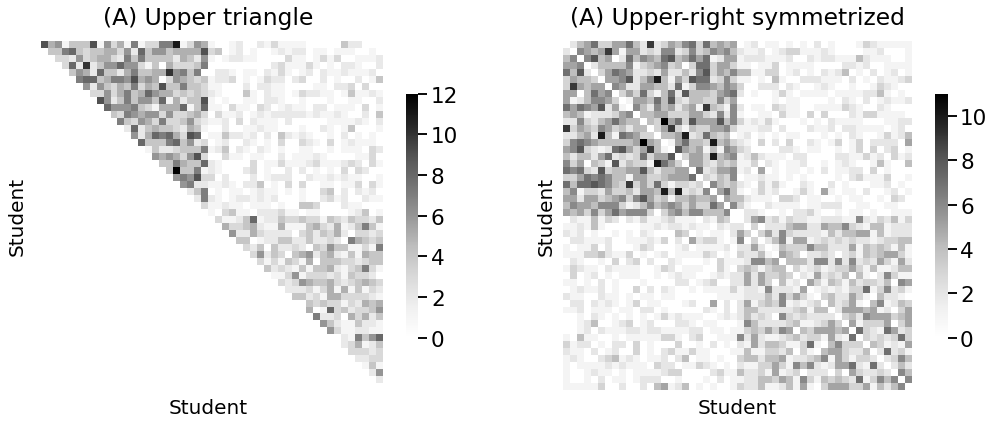
\includegraphics[width=\linewidth]{representations/ch4/Images/triusym.png}
    \caption[Symmetrization through discarding a triangle]{The matrices \texttt{A\_activity\_uppertri} and \texttt{A\_activity\_triu\_symmetrized} showing the \textbf{(A)} upper triangle, \textbf{(B)} and upper-right symmetrized adjacency matrices.}
    \label{fig:ch4:triusym}
\end{figure}
Likewise, if the network only had the lower triangle stored, you could do the same thing but with\texttt{method="tril"} to retain the lower triangle of the matrix.

\paragraph{Taking a function of the two values}

There are many other ways you use a function of $a_{ij}$ and $a_{ji}$ to get a symmetric matrix (and an undirected network). One is to just average. That is, you can let the matrix $A'$ be the matrix with entries $a'_{ij} = \frac{a_{ij} + a_{ji}}{2}$ for all $i$ and $j$. In matrix form, this operation looks like this:

\begin{align*}
    A' &= \frac{1}{2} (A + A^\top) \\
    &= \frac{1}{2}\left(\begin{bmatrix}
        a_{11} & ... & a_{1n} \\
        \vdots & \ddots & \vdots \\
        a_{n1} & ... & a_{nn}
    \end{bmatrix} + \begin{bmatrix}
        a_{11} & ... & a_{n1} \\
        \vdots & \ddots & \vdots \\
        a_{1n} & ... & a_{nn}
    \end{bmatrix}\right)\\
    &= \begin{bmatrix}
        \frac{1}{2}(a_{11} + a_{11}) & ... & \frac{1}{2}(a_{1n} + a_{n1}) \\
        \vdots & \ddots & \vdots \\
        \frac{1}{2} (a_{n1} + a_{1n}) & ... & \frac{1}{2}(a_{nn} + a_{nn})
    \end{bmatrix} \\
    &= \begin{bmatrix}
        a_{11} & ... & \frac{1}{2}(a_{1n} + a_{n1}) \\
        \vdots & \ddots & \vdots \\
        \frac{1}{2} (a_{n1} + a_{1n}) & ... & a_{nn}
    \end{bmatrix}
\end{align*}
As you can see, for all of the entries, $a'_{ij} = \frac{1}{2} (a_{ij} + a_{ji})$, and also $a_{ji}' = \frac{1}{2}(a_{ji} + a_{ij})$. These quantities are the same, so $a_{ij}' = a_{ji}'$, and $A'$ is symmetric. As the adjacency matrix is symmetric, the network that $A'$ represents is undirected.

Remember that the asymmetry in the friendship network means student $i$ might perceive their friendship with student $j$ as being stronger or weaker than student $j$ perceived about student $i$. What you did here was instead of just arbitrarily throwing one of those values away, you said that their friendship might be better indicated by averaging the two values. This produced for us a single friendship strength $a_{ij}'$ where $a_{ij}' = a_{ji}'$.

You can implement this in graspologic as follows:
\begin{lstlisting}[style=python]
# symmetrize with averaging
A_friend_avg_sym = symmetrize(A_friend, method="avg")
\end{lstlisting}
We'd encourage you to plot the outcome and convince yourself that it is, in fact, symmetric using the \texttt{is\_symmetric()} function you learned about in the last section.

We'll will use the friendship network symmetrized by averaging (\texttt{A\_friend\_avg\_sym}) in several of the below examples, which we will call the ``undirected friendship network''.

\subsubsection{Diagonal augmentation}
\label{sec:ch4:regularization:diag_aug}

In your future works with network machine learning, you will come across numerous techniques which operate on adjacency matrices which are \emph{positive semi-definite}. This word doesn't need to mean a whole lot to you conceptually, but it has a big implication when you try to use algorithms on many of your networks. Remember that when you have a loopless network, a common practice in network science is to set the diagonal to zero. What this does is it leads to your adjacency matrices being \emph{indefinite} (which means, \emph{not} positive semi-definite). For our purposes, this means that many network machine learning techniques simply cannot operate on these adjacency matrices. However, as we mentioned before, these entries are not actually zero, but simply \emph{do not exist} and you just didn't have a better way to represent them. Or do you?

\emph{Diagonal augmentation} is a procedure for imputing the diagonals of adjacency matrices for loopless networks. This gives us "placeholder" values that do not cause this issue of indefiniteness, and allow your network machine learning techniques to still work. Remember that for a simple network, the adjacency matrix will look like this:
\begin{align*}
    A &= \begin{bmatrix}
        0 & a_{12} & ... & a_{1n} \\
        a_{21}& \ddots & & \vdots \\
        \vdots & & \ddots & a_{n-1, n} \\
        a_{n1} &...& a_{n, n-1} & 0
    \end{bmatrix}
\end{align*}

What you do is impute the diagonal entries using the \emph{fraction of possible edges which exist} for each node. This quantity is simply the node degree $d_i$ (the number of edges which exist for node $i$) divided by the number of possible edges node $i$ could have (which would be node $i$ connected to each of the other $n-1$ nodes). Remembering that the degree matrix $D$ is the matrix whose diagonal entries are the degrees of each node, the diagonal-augmented adjacency matrix is given by:
\begin{align*}
    A' &= A + \frac{1}{n-1}D = \begin{bmatrix}
        \frac{d_1}{n-1} & a_{12} & ... & a_{1n} \\
        a_{21}& \ddots & & \vdots \\
        \vdots & & \ddots & a_{n-1, n} \\
        a_{n1} &...& a_{n, n-1} & \frac{d_n}{n-1}
    \end{bmatrix}
\end{align*}
When the matrices are directed or weighted, the computation is a little different, but fortunately \texttt{graspologic} will handle this for us. Let's see how you would apply this to the directed friendship network:
\begin{lstlisting}[style=python]
from graspologic.utils import augment_diagonal

A_friend_aug = augment_diagonal(A_friend)
\end{lstlisting}
We will rotate back to the problem of positive semi-definiteness in Section \ref{sec:ch5:psd_block} as it relates to statistical models for networks, and will pivot back again in Section \ref{sec:ch6:spectral} for what it means with regard to adjacency matrices.

\subsection{Regularizing the edges of weighted networks}

As you are probably aware, in all of machine learning, you are always concerned with the \emph{bias/variance tradeoff}. The \textit{bias/variance tradeoff} is an unfortunate side-effect that concerns how well a learning technique will generalize to new datasets \cite{Hastie2009}.
\begin{enumerate}
    \item \textit{Bias} is an error from erroneous assumptions you make about the system that you are learning about. For instance, if you have a friendship network, you might make simplifying assumptions, such as an assumption that two athletes frorm different sports have an equally likely chance of being friends with a member of the band. This might be flat out false, as band members might be selectively better friends with athletes depending on which sports they play.
    \item On the other hand, the \textit{variance} is the degree to which the an estimate of a task will change when given new data. An assumption that if a player is a football player he has a higher chance of being friends with a band member might make sense given that the band performs at football games. 
\end{enumerate}

The "trade-off" is that these two factors tend to be somewhat at odds, in that raising the bias tends to lower the variance, and vice-versa:
\begin{enumerate}
    \item \textit{High bias, but low variance}: Whereas a lower variance model might be better suited to the situation where the data you expect to see is noisy, it might not as faithfully represent the underlying dynamics you think the network possesses. A low variance model might ignore that athletes might have a different chance of being friends with a band member based on their sport all together. This means that while you won't get the student relationships \emph{correct}, you might still be able to get a reasonable estimate that you think is not due to overfitting. In this case, you've smoothed away \emph{signal} from the data at the expense of avoiding \emph{noise}.
    \item \textit{Low bias, but high variance}: Whereas a low bias model might more faithfully model true relationships in your training data, it might fit your training data a little \emph{too} well. Fitting the training data too well is a problem known as \textit{overfitting}. If you only had three football team members and tried to assume that football players were better friends with band members, you might not be able to well approximate this relationship because of how few individuals you have who reflect this situation. 
\end{enumerate}

Here, we show several strategies to reduce the variance (but, add bias) due to edge weight noise in network machine learning.

\subsubsection{Sparsification of the network}

The procedure of \textit{sparsification} is one in which we take a network, and we remove edges from it, which is described by \cite{Spielman2008Aug} and \cite{Batson2013Aug}. Remember that removing edges, in terms of the adjacency matrix, is analogous to setting the corresponding adjacencies to zero. A matrix with many entries of zero is called a \emph{sparse} matrix. So, the reason we call the removal of the edges from a network \emph{sparsification} is that we are producing a network with a \emph{sparse} adjacency matrix.

\emph{Sparsification} is a general class of edge regularization techniques, and includes many flavors. Here, we discuss a few of them. In network sparsification, we will often pick some property of the network (such as, a particular edge weight) and remove edges in an attempt to preserve something about this particular property.

A useful tool to study for how, exactly, you might want to go about sparsifying the network is called the \emph{edge-weight distribution} of your network sample. The edge-weight distribution of the network sample are the particular values that the edge weights of the network take. The most common way to visualize the edge-weight distribution is an edge-weight histogram. This is very similar to the node-degree histogram you worked with above, but instead of node degrees, you look at the edge-weights. Let's take a look at the friendship network, and then take a look at its edge-weight distribution. Remember that the friendship network is \emph{undirected}, so we need to remove its diagonal elements \emph{before} we visualize the edge-weight distribution. We'll also remove edges with zero-weights for visualization purposes:

\begin{lstlisting}[style=python]
def discard_diagonal(A):
    """
    A function that discards the diagonal of a matrix,
    and returns its non-diagonal edge-weights.
    """
    # create a mask that is True for the non-diagonal edges
    non_diag_idx = np.where(~np.eye(A.shape[0], dtype=bool))
    return A[non_diag_idx].flatten()

friend_nondiag_ew = discard_diagonal(A_friend)
# get the non-zero, non-diagonal edge weights
friend_nondiag_nz_ew = friend_nondiag_ew[friend_nondiag_ew > 0]

# plot the histogram, as above
histplot(friend_nondiag_nz_ew, bins=20, binrange=(0, 1))
\end{lstlisting}
We show this plot in Figure \ref{fig:ch4:truncate}(C).

\begin{figure}[h]
    \centering
    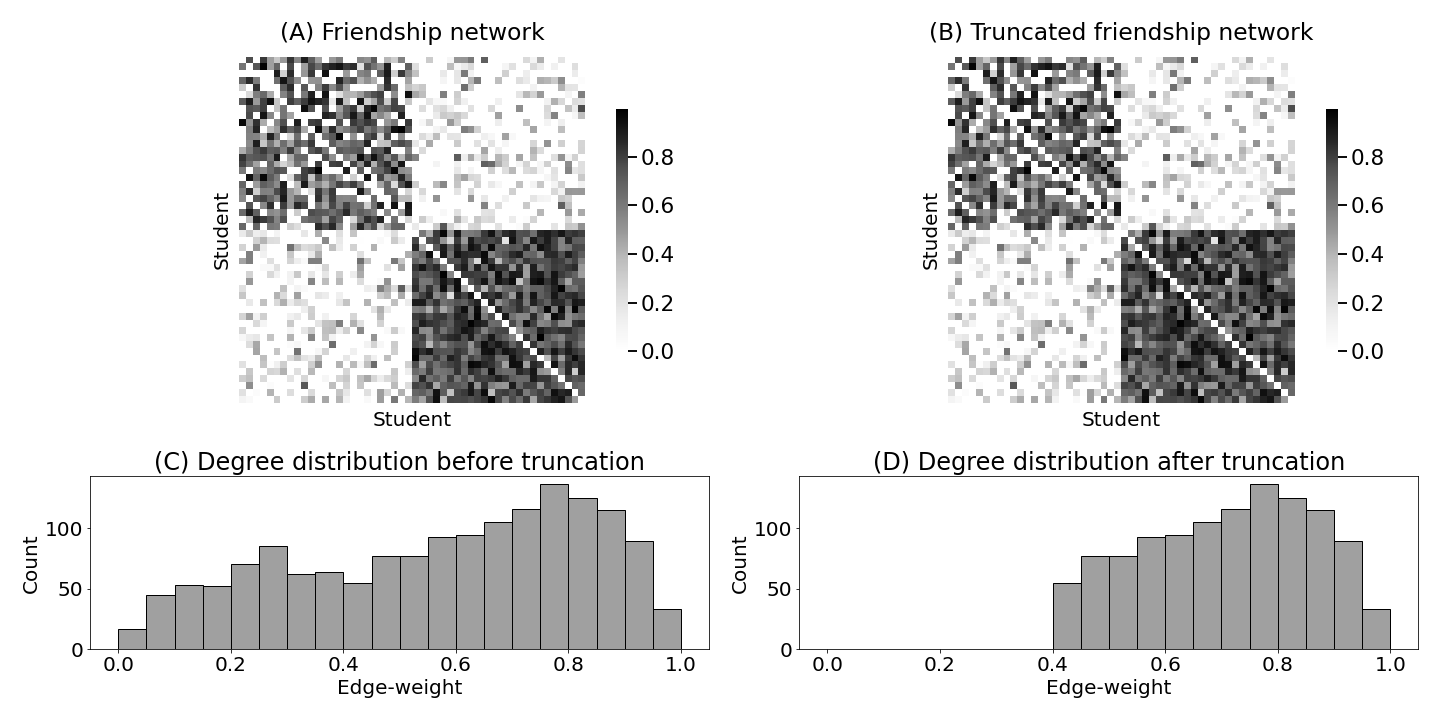
\includegraphics[width=\linewidth]{representations/ch4/Images/truncate.png}
    \caption[Truncation]{\textbf{(A)} The adjacency matrix before truncation. \textbf{(B)} The adjacency matrix after truncation. \textbf{(C)} The non-zero, non-diagonal edge weights before truncation. \textbf{(D)} The non-zero, non-diagonal edge weights after truncation.}
    \label{fig:ch4:truncate}
\end{figure}

\paragraph{Truncation removes the smallest edges}

The simplest way to reduce the variance due to edge weight noise is called \emph{edge truncation}. \textit{Edge truncation} is a process by which you choose some threshold value $\tau$, and remove all of the weights which are smaller than $\tau$ but retain the weights that are bigger than $\tau$. For edges that are equal to $\tau$, what you'll want to do depends on the strategy you are employing. We'll arbitrarily set nodes $\leq \tau$ to zero in our case, but you might use $\geq \tau$ in your uses.

So, how is $\tau$ typically chosen? There are a few ways, but it's usually one of the below two:
\begin{enumerate}
    \item Choose $\tau$ arbitrarily: after looking at your network and doing some preliminary visualizations, you might determine that your edge weights tend to be ``multi-modal''. This means that when you look at the edge-weight distribution, you see multiple "clusters" of edge weight bins which are larger, or smaller. For a lot of networks, these small edges might be very noise induced; that is, the small edges might just spuriously be close to, but {not quite}, zero, due to errors in your measuring process. When the edge weights are really tiny, you might think that these noisy edges are better off just not existing.
    \item Choose $\tau$ based on a particular quantile: A \textit{quantile} is a percentile divided by $100$. In this strategy, you identify a target quantile of the edge-weight distribution. What this means is that you are selecting the lowest {fraction} of the edge-weights (where that fraction is the quantile that you choose) and setting these edges to $0$, and selecting the remaining edges are left unchanged. If you select a quantile of $0.5$, this means that you take the smallest $50\%$ of edges and set them to zero, and the largest $50\%$ of edges and retain their initial value. There are three potential pitfalls to quantiling, which we elaborate on below.
\end{enumerate}
This is called \emph{truncation} because you are taking the edge-weight distribution, and \emph{truncating} (cutting it off) below the value $\tau$.

With respect to what to do with edges that are equal to $\tau$, when you choose a threshold arbitrarily, you can do whatever you want with them, as long as you are consistent if you have multiple networks you are truncating. What we mean by this is that you can select to remove edges less than or equal to this threshold, or retain edge weights greater than or equal to the threshold. When you truncate on the basis of a quantile, however, this is not quite the case. You will want to remove all the edges below $\tau$, and truncate away the remaining edges equal to $\tau$ at random until you have truncated the desired fraction of edges in total.

Let's see how this works in practice. In the edge-weight histogram, in Figure \ref{fig:ch4:truncate} you can notice two "peaks" to the non-zero edge-weights.

If you think that the smaller peak edge-weights are spurious/noise, you might want to threshold somewhere in between the smaller and the larger peaks, like near $0.4$, which is highlighted in \ref{fig:ch4:truncate}(C). 

\begin{lstlisting}[style=python]
def truncate_network(A, threshold):
    A_cp = np.copy(A)
    A_cp[A_cp <= threshold] = 0
    return A_cp

tau = 0.4
A_friend_trunc = truncate_network(A_friend, threshold=tau)
\end{lstlisting}
The next thing to look at is the adjacency matrix, before and after truncation. We show these plots in Figure \ref{fig:ch4:truncate}(A) and \ref{fig:ch4:truncate}(B). Notice that the smallest weight edges in the network (in this case, the ones with edge weights $\leq 0.4$) have been replaced with zeros. As you can see, a lot of the edges in the upper right and upper left, which were previously small, are now \emph{zero}. This is reflected in the edge-weight distribution:

\begin{lstlisting}[style=python]
friend_trunc_nondiag_ew = discard_diagonal(A_friend_trunc)
# get the non-zero, non-diagonal edge weights
friend_trunc_nondiag_nz_ew = friend_trunc_nondiag_ew[friend_trunc_nondiag_ew > 0]
histplot(friend_trunc_nondiag_nz_ew, bins=20, binrange=(0, 1))
\end{lstlisting}
which is shown in Figure \ref{fig:ch4:truncate}(D). As you can see, all of the edges with weights less than $\tau = 0.4$ have been truncated away.

A slight caveat to this procedure we learned about above for truncation is that, if you use the quantile approach and the network is undirected, you need to exclude one triangle of the network to obtain the appropriate quantile. This is because when $a_{ij} = a_{ji}$, you would otherwise count an edge twice if you just used the adjacency matrix to obtain quantiles. We'll see this more in the example on thresholding below.


\paragraph{Thresholding converts weighted networks to unweighted networks}
\label{sec:ch4:regularization:thresholding}

Closely related to truncation is the process of \emph{thresholding}. Like truncation, you begin with a threshold $\tau$, which is usually chosen arbitrarily or based on a quantile, like for truncation. However, there is one key difference: when you threshold a network, you set the edges below $\tau$ to zero, and the edges greater than $\tau$ to \emph{one}. This has the effect of taking a weighted network, and effectively transforming it into an undirected network. 

We will show how to use the quantile approach to thresholding, with the activity/hobby network. You will threshold by choosing $\tau$ such that $\tau$ is the value which is the $0.3$ quantile, or the $30$ percentile, of the edge-weight distribution. Remember as you learned in the preceding section, that if the network itself is loopless, the diagonal entries simply \emph{do not exist}; $0$ is simply a commonly used placeholder. For this reason, when you compute quantiles of edge-weights, you need to \emph{exclude the diagonal} if the network is loopless. 

\begin{floatingbox}[h]\caption{Why is thresholding with a quantile desirable?}\label{box:ch4:desirable}
Remember that in Section \ref{sec:ch4:prop-net:density}, we defined the network density for a simple network as:

\begin{align*}
    density(A) &= \frac{\sum_{j > i}a_{ij}}{\binom{n}{2}}.
\end{align*}

If you threshold this network at a quantile of $q$, this means you will, ideally, set $1 - q$ fraction of the edges to $1$, and a $q$ fraction of the edges to zero.

If we are able to do this perfectly, then $\sum_{j > i}a_{ij} = (1 - q)\binom n 2$.

Therefore:
\begin{align*}
    density(A) &= \frac{(1 - q)\binom n 2}{\binom n 2} = 1 - q
\end{align*}

So when you threshold the network at a quantile $q$, and you are {actually} able to set a $q$ fraction of the edges to zero and a $1 - q$ fraction of the edges to one, you end with a network of density equal to $1 - q$. We will see a for conditions as to when this will, and will not, occur later.
\end{floatingbox}

Further, since this network is undirected, you also need to restrict your attention to one triangle of the corresponding adjacency matrix. We choose the upper-right triangle arbitrarily, as the adjacency matrix's symmetry means the upper-right triangle and lower-right triangle have identical edge-weight distributions. We can do this using \texttt{numpy}. This network is loopless and undirected, so we will want to exclude both the diagonal {and} only perform our analysis on a single triangle of the matrix:
\begin{lstlisting}[style=python]
# find the indices which are in the upper triangle and not in the diagonal
upper_tri_non_diag_idx = np.where(np.triu(np.ones(A_activity.shape), k=1).astype(bool))
q = 0.3  # desired quantile is 0.5, or 50 percentile
histplot(A_activity[upper_tri_non_diag_idx].flatten())
tau = np.quantile(A_activity[upper_tri_non_diag_idx], q=q)
\end{lstlisting}

So, let's see what happens when we just compute $\tau$ using the $q$ quantile of the non-diagonal, upper triangular entries of $A$, and then threshold $A$ using $\tau$. To do this, we'll just check the number of edges greater than $\tau$, and the number less than or equal to $\tau$. Since we used $q = 0.5$ as our desired quantile, we should anticipate that these numbers should be very close to equal:

\begin{lstlisting}[style=python]
n_lteq_tau = np.sum(A_activity[upper_tri_non_diag_idx] <= tau)
n_gt_tau = np.sum(A_activity[upper_tri_non_diag_idx] > tau)
print("Number of edges less than or equal to tau: {}".format(n_lteq_tau))
print("Number of edges greater than to tau: {}".format(n_gt_tau))
\end{lstlisting}
While the specific results you obtain will depend on your specific computer since we used random simulation data here, you're going to get numbers that are not even close to equal (the number of edges $\leq \tau$ should be about 50\% larger than the number of edges $> \tau$). So what happened?

\paragraph{The duplicate value pitfall}

Let's imagine an array that was \texttt{[1,2,3,4]} and \texttt{[1,2,2,4]}, and we chose the $0.5$ quantile, the first array would give a $0.5$ quantile of \texttt{2.5}. If we thresholded with this value, we would get \texttt{[0,0,1,1]}, and the number of elements retained after thresholding would be $50\%$ ones and $50\%$ zeros, like we expected. On the other hand, the $0.5$ quantile of the second array is \texttt{2}, and if we used the thresholding approach above we would get \texttt{[0,0,0,1]}, which has $75\%$ of the values taking $0$ and $25\%$ of the values taking one. 

This means that if you pass in a quantile $q$ and you expect that $q$ fraction of the points will have a value of $0$ after truncation/thresholding, you are going to need to be very careful with your data to handle points that are \emph{equal} to your quantile. To do this, one way is to assign edges less than $\tau$ to zero, and the edges greater than $\tau$ to one. Then, for edges equal to $\tau$, you can to randomly assign them to a zero or one, until you obtain the desired quantiling threshold. This can be done with the pseudocode in Algorithm \ref{alg:ch4:thresholding}. You could write a similar utility for truncating at a quantile.

\begin{algorithm}[h]
    \SetAlgoLined
    \caption{Thresholding an adjcency matrix with random tiebreaking.}
    \label{alg:ch4:thresholding}
    \KwData{$A$: an adjacency matrix \newline $q$: a quantile between $0$ and $1$}
    \KwResult{an adjacency matrix thresholded at the $q$ quantile.}
    Let $d$ be the minimum non-zero difference between any two elements of $A$.
    
    \For{$i$ in $1$ : $n$}{
        \For{$j$ in $1$ : $n$}{
            Let $\epsilon_{ij}$ be a random number between $0$ and $d$.
        }
    }

    \If{$A$ is symmetric}{
        $\epsilon = \frac{\epsilon + \epsilon^\top}{2}$
    }

    Compute the augmented adjacency matrix, $A' = A + \frac{\epsilon}{10}$.

    Compute the appropriate threshold $\tau$ using $A'$.

    Threshold $A'$ by setting elements where $a_{ij}' > \tau$ to one, and $a_{ij}' < \tau$ to zero.
\end{algorithm}

Basically, what this algorithm does is it adds a very small amount of noise to the matrix $A$ that you are thresholding. Note that we take care to ensure that if $A$ is symmetric and the network is undirected, that we add the \emph{same} amount of noise to both entries $a_{ij}$ and $a_{ji}$ by \emph{symmetrizing} this ``noise matrix'' $\epsilon$. This noise is small enough that it is an order of magnitude (a factor of $10$) smaller than the smallest appreciable difference in any two non-zero elements of $A$. 

After we add this matrix to $A$, there is a probability of \emph{zero} that any two elements of $A$ will have the same value. Further, since we added noise that was an order of magnitude smaller than any non-zero differences of elements of $A$, it is impossible for an item that was originally greater than a quantile to now be less than the desired quantile, and vice-versa. This strategy is called a random tiebreaking, since we broke ties that occur at exactly the $q$ quantile randomly.

This can be implemented in python as follows:

\begin{lstlisting}[style=python]
from numpy import copy

def min_difference(arr):
    b = np.diff(np.sort(arr))
    return b[b>0].min()

def quantile_threshold_network(A, directed=False, loops=False, q=0.5):
    # a function to threshold a network on the basis of the
    # quantile
    A_cp = np.copy(A)
    n = A.shape[0]
    E = np.random.uniform(low=0, high=min_difference(A)/10, size=(n, n))
    if not directed:
        # make E symmetric
        E = (E + E.transpose())/2
    mask = np.ones((n, n))
    if not loops:
        # remove diagonal from E
        E = E - np.diag(np.diag(E))
        # exclude diagonal from the mask
        mask = mask - np.diag(np.diag(mask))
    Ap = A_cp + E
    tau = np.quantile(Ap[np.where(mask)].flatten(), q=q)
    A_cp[Ap <= tau] = 0; A_cp[Ap > tau] = 1
    return A_cp

A_activity_thresholded03 = quantile_threshold_network(A_activity, q=0.3)
A_activity_thresholded07 = quantile_threshold_network(A_activity, q=0.7)
\end{lstlisting}
We visualize these two thresholded adjacency matrices along with the unweighted adjacency matrix in Figure \ref{fig:ch4:threshold_res}.

\begin{figure}[h]
    \centering
    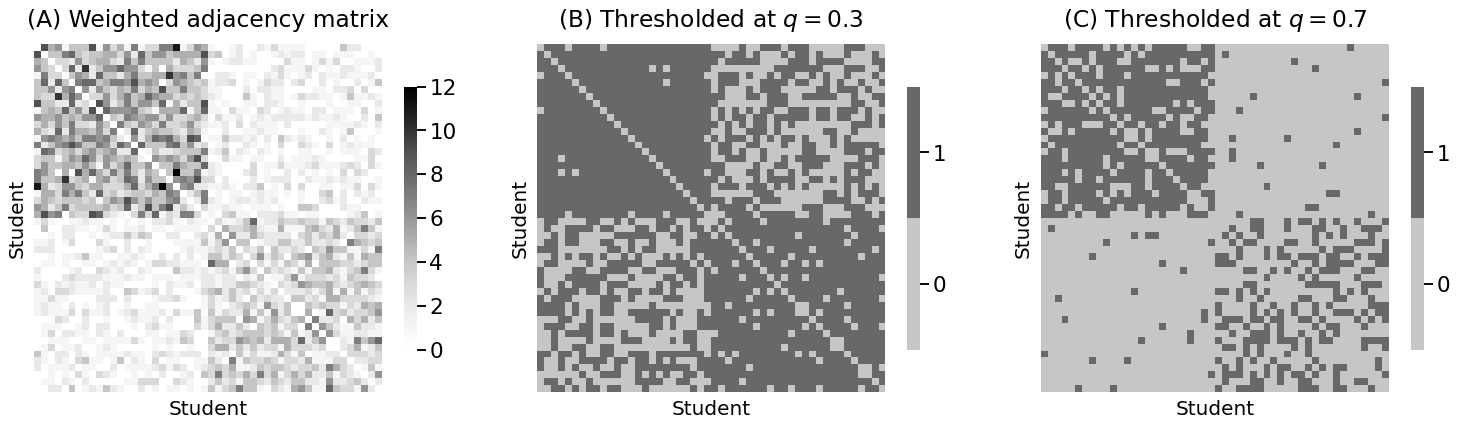
\includegraphics[width=\linewidth]{representations/ch4/Images/threshold_res.png}
    \caption[Thresholding]{\textbf{(A)} the weighted adjacency matrix of the activity/hobby network. \textbf{(B)} the weighted adjacency matrix of the activity/hobby network after thresholding at $0.3$. \textbf{(C)} the weighted adjacency matrix of the activity/hobby network after thresholding at $0.7$.}
    \label{fig:ch4:threshold_res}
\end{figure}

Great job. Now, let's just confirm that we didn't run into the duplicate value pitfall. We'll do this by writing a utility which computes the network density from an adjacency matrix for a simple network:

\begin{lstlisting}[style=python]
from graspologic.utils import is_unweighted, is_loopless, is_symmetric

def simple_network_dens(X):
    # make sure the network is simple
    if (not is_unweighted(X)) or (not is_loopless(X)) or (not is_symmetric(X)):
        raise TypeError("Network is not simple!")
    # count the non-zero entries in the upper-right triangle
    # for a simple network X
    nnz = np.triu(X, k=1).sum()
    # number of nodes
    n = X.shape[0]
    # number of possible edges is 1/2*n*(n-1)
    poss_edges = 0.5*n*(n-1)
    return nnz/poss_edges

print("Network Density: {:.3f}".format(simple_network_dens(A_activity_thresholded03)))
# Network Density: 0.700
\end{lstlisting}

So our solution achieved the desired network density.

We call this pitfall the \emph{duplicate value pitfall} because you can \emph{only} run into it if your adjacency matrix has the same value duplicated.

\paragraph{The ``underly ambitious'' pitfall}

The next pitfall of using a quantile $q$ is actually a special case of the duplicate value pitfall listed above: you might choose an underly ambitious quantile to truncate/threshold with. By underly ambitious, what we mean is that the adjacency matrix doesn't even have a $1 - q$ fraction of non-zero edges. When you threshold $A$ with a quantile of $q$, you can spot this pitfall fairly easily by simply checking the fraction of $0$-weight edges ahead of time.

For an example, let's consider a network where $50\%$ of the possible edges are zero (the network density is $0.5$, and the other $50\%$ are one. If you were to choose a quantile of $0.3$, quantiling will still only give you a network density of $0.5$, and not $0.7$ like you might have expected from Remark \ref{box:ch4:desirable}.

Unfortunately, there's no quick fix like there was for the non-continuous pitfall; if you run into the underly ambitious pitfall and tried to use the randomization procedure, the ``solution'' would end up setting edges with a value of zero in the adjacency matrix to one, which doesn't make much sense. To avoid this pitfall, you need to analyze your densities ahead of time if you want to use quantiling, and ensure that the quantile you choose is not underly ambitious. 

If you had a collection of networks that you wanted to threshold or truncate \emph{en masse} using a quantile $q$, you could do this by plotting a histogram of your network densities, and ensuring that $1 - q$ is less than all of the network densities in your collection.

\begin{floatingbox}[h]\caption{With all these pitfalls, why would we quantile?}
As we mentioned in Section \ref{sec:ch4:net-rep:featurelims}, many network summary statistics that you might be interested in could be heavily correlated with the network density. For this reason, if you want to analyze a collection of networks using summary statistics, it might make sense to analyze a collection of networks with the same network density. This is because in some sense, analyzing the networks with a similar network density will ``decouple'' this correlation with the network density, since the network density will no longer be changing across the networks.
\end{floatingbox}

\paragraph{When can we ignore these pitfalls entirely?}

As you might be able to gather from the above, if our network fulfills two properties, we are guaranteed that we won't run into the quantiling pitfalls. First, if the network is \textit{dense} (a network where all possible entries $a_{ij}$ are non-zero, with arbitrarily small or large edge-weights), we cannot possibly run into the underly ambitious pitfall, since that pitfall will only arise when there are zero-weight edges in the adjacency matrix. Second, if the adjacency matrix does not have any duplicate values, we cannot run into the duplicate value pitfall either, because we cannot have ties at the desired quantile if there are no duplicated values in the edge weights. 

As we have repeated many times in this section, when considering when a network might run into these pitfalls using the adjacency matrix, be sure to only consider appropriate entries of the adjacaency matrix. This means restricting your analysis to the upper triangle or the lower triangle if the netework is undirected, and removing the diagonal if the network is loopless. 

\subsubsection{Edge-weight global rescaling}

With weighted networks, it is often the case that you might want to reshape the distributions of edge-weights in your networks to highlight particular properties. Notice that the edge-weights for your friendship network takes values between $0$ and $1$, but your activity network takes values between $0$ and almost $15$. How can you possibly compare between these two networks where the edge-weights take such different ranges of values? You turn to standardization, which allows us to place values from different networks on the same scale. 

\paragraph{$z$-scoring standardizes edge weights using the normal distribution}

The first approach to edge-weight standardization is known commonly as $z$-scoring. Suppose that $A$ is the adjacency matrix, with entries $a_{ij}$. With a $z$-score, you will rescale the weights of the adjacency matrix, such that the new edge-weights (called $z$-scores) are approximately normally distributed. The reason this can be useful is that the normal distribution is pretty ubiquitous across many branches of science, and therefore, a $z$-score is relatively easy to communicate with other scientists. Further, many things that exist in nature can be well-approximated by a normal distribution, so it seems like a reasonable place to start to use a $z$-score for edge-weights, too! The $z$-score is defined as follows. You will construct the $z$-scored adjacency matrix $Z$, whose entries $z_{ij}$ are the corresponding $z$-scores of the adjacency matrix's entries $a_{ij}$. For a weighted, loopless network, you use an estimate of the \emph{mean}, $\hat \mu$, and the \emph{unbiased} estimate of the \emph{variance}, $\hat \sigma^2$, which can be computed as follows:
\begin{align*}
    \hat\mu &= \frac{1}{n(n-1)}\sum_{i \neq j}a_{ij},\\
    \hat\sigma^2 &= \frac{1}{n(n - 1) - 1}\sum_{i \neq j} (a_{ij} - \hat\mu)^2.
\end{align*}
The $z$-score for the $(i,j)$ entry is simply the quantity:
\begin{align*}
    z_{ij} &= \frac{a_{ij} - \hat\mu}{\hat\sigma}
\end{align*}
Since your network is loopless, notice that these sums are for all \emph{non-diagonal} entries where $i \neq j$. If the network were not loopless, you would include diagonal entries in the calculation, and instead would sum over all possible combinations of $i$ and $j$. the interpretation of the $z$-score $z_{ij}$ is the \emph{number of stadard deviations} that the entry $a_{ij}$ is from the mean, $\hat \mu$.

We will demonstrate on the directed friendship network. You can implement $z$-scoring as follows:

\begin{lstlisting}[style=python]
from scipy.stats import zscore

def z_score_loopless(X, undirected=False):
    if not is_loopless(X):
        raise TypeError("The network has loops!")
    if is_symmetric(X):
        raise TypeError("The network is undirected!")
    # the entries of the adjacency matrix that are not on the diagonal
    non_diag_idx = np.where(~np.eye(X.shape[0], dtype=bool))
    Z = np.zeros(X.shape)
    Z[non_diag_idx] = zscore(X[non_diag_idx])
    return Z

ZA_friend = z_score_loopless(A_friend)
\end{lstlisting}

The theory for when, and why, to use $z$-scoring for network machine learning tends to go something like this: many things tend to be normally distributed with the same mean and variance, so perhaps that is a reasonable expectation for your network, too. Unfortunately, we find this often to \emph{not} be the case. In fact, we often find that the specific distribution of edge weights itself often might be lamost infeasible to identify in a population of networks, and therefore \emph{almost} irrelevant all-together. To this end, we turn to instead \emph{ranking} the edges.

Note that in the above code snippet, we throw an error if the network is undirected (and the adjacency matrix is symmetric): remember that you want to be careful to restrict your analysis to the upper triangle if the network is undirected and loopless. This won't really change the estimate of the mean, but the variance will be slightly different. The sums would be over $j > i$, and the normalizing factors would be $\binom n 2$ instead of $n(n - 1)$.

\paragraph{Ranking edges preserves ordinal relationships}

The idea behind ranking is as follows. You don't really know much useful information as to how the distribution of edge weights varies between a given pair of networks. For this reason, you want to virtually eliminate the impact of that distribution \emph{almost} entirely. However, you know that if one edge-weight is larger than another edge-weight, that you do in fact trust that relationship. What this means is that you want something which preserves \emph{ordinal} relationships in your edge-weights, but ignores other properties of the edge-weights. An ordinal relationship just means that you have a natural ordering to the edge-weights. This means that you can identify a largest edge-weight, a smallest edge-weight, and every position in between. When we want to preserve ordinal relationships in your network, we do something called \emph{passing the non-zero edge-weights to ranks}. We will often use the abbreviation\texttt{ptr} to define this function because it is so useful for weighted networks. We pass non-zero edge-weights to ranks as in Algorithm \ref{alg:ch4:ptr}.

\begin{algorithm}[h]
    \SetAlgoLined
\caption{Passing an adjacency matrix to ranks}
\label{alg:ch4:ptr}
    \KwData{$A$ is an adjacency matrix.}
    \KwResult{The adjacency matrix, after passing to ranks.}
    Identify all of the non-zero entries of the adjacency matrix $A$.

    Let $n_{nz}$ be the number of non-zero entries of the adjacency matrix $A$.

    Rank all of the non-zero edges in the adjacency matrix $A$, where for a non-zero entry $a_{ij}$, $rank(a_{ij}) = 1$ if $a_{ij}$ is the smallest non-zero edge-weight, and $rank(a_{ij}) = n_{nz}$ if $a_{ij}$ is the largest edge-weight. Ties are settled by using the average rank of the tied entries.

    Report the weight of each non-zero entry $(i,j)$ as $r_{ij} = \frac{rank(a_{ij})}{n_{nz} + 1}$, and for eachh zero entry as $r_{ij} = 0$.
\end{algorithm}

Below, we pass-to-ranks the directed friendship network using\texttt{graspologic}:

\begin{lstlisting}[style=python]
from graspologic.utils import pass_to_ranks

RA_friend = pass_to_ranks(A_friend)
\end{lstlisting}

A plot of the adjacency matrices before and after passing to ranks, as well as the edge-weight histograms before and after passing to ranks, is shown in Figure \ref{fig:ch4:ptr}.

\begin{figure}[h]
    \centering
    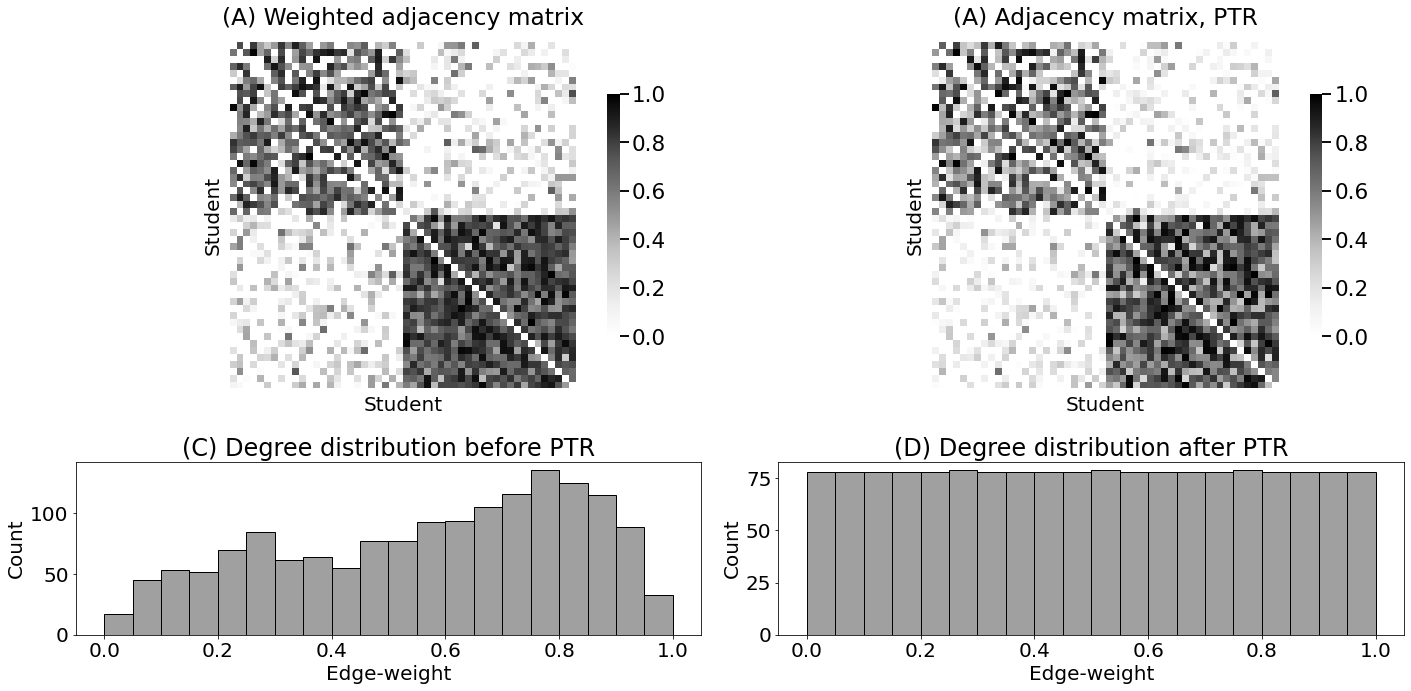
\includegraphics[width=\linewidth]{representations/ch4/Images/ptr.png}
    \caption[Passing to ranks to normalize edge-weights]{\textbf{(A)} the adjacency matrix before passing to ranks for the friendship network. \textbf{(B)} the adjacency matrix after passing to ranks. \textbf{(C)} the edge-weight histogram (including zero-weight edges) before passing to ranks. \textbf{(D)} the edge-weight histogram (including zero-weight edges) after passing to ranks.}
    \label{fig:ch4:ptr}
\end{figure}
The edge-weights for the adjacency matrix $R$ after \texttt{ptr} has the interpretation that each entry $r_{ij}$ which is non-zero is the \emph{quantile} of that entry amongst \emph{the other non-zero entries}. This is unique in that it is completely \emph{distribution-free}, which means that you don't need to assume anything about the distribution of the edge-weights to have an interpretable quantity. On the other hand, the $z$-score had the interpretation of the number of standard deviations from the mean, which is only a sensible quantity to compare if you assume the population of edge-weights are normally distributed.


Another useful quantity related to pass-to-ranks is known as the zero-boosted pass-to-ranks. Zero-boosted pass-to-ranks is conducted as in Algorithm \ref{alg:ch4:ptr_zb}.

\begin{algorithm}[h]
\SetAlgoLined
\caption{Zero-boosted pass to ranks}
    \KwData{$A$ is an adjacency matrix.}
    \KwResult{The adjacency matrix, after passing to ranks.}
    Identify all of the non-zero entries of the adjacency matrix $A$ and the zero-weighted entries of the adjacency matrix $A$.

    Let $n_{nz}$ be the number of non-zero entries of the adjacency matrix $A$, and $n_z$ be the number of zero-weighted entries of the adjacency matrix $A$. Note that $n_{nz} + n_z = n^2$, since $A$ has $n^2$ entries.

    Rank all of the non-zero edges in the adjacency matrix $A$, where for a non-zero entry $a_{ij}$, $rank(a_{ij}) = 1$ if $a_{ij}$ is the smallest non-zero edge-weight, and $rank(a_{ij}) = n_{nz}$ if $a_{ij}$ is the largest edge-weight. Ties are settled by using the average rank of the two entries.

    Report the weight of each non-zero entry $(i,j)$ as $r_{ij}' = \frac{n_z + rank(a_{ij})}{n^2 + 1}$, and for each zero entry as $r_{ij}' = 0$.
\end{algorithm}

The edge-weights for the adjacency matrix $R'$ after zero-boosted\texttt{ptr} have the interpretation that each entry $r_{ij}'$ is the quantile of that entry amongst \emph{all} of the entries. Let's instead use zero-boosted\texttt{ptr} on your network:

\begin{lstlisting}[style=python]
RA_friend_zb = pass_to_ranks(A_friend, method="zero-boost")
\end{lstlisting}
We show the adjacency matrix after zero-boosted \texttt{ptr}, along with the edge-weight histogram (including zero-weight edges), in Figure \ref{fig:ch4:ptr_zb}.

\begin{figure}[h]
    \centering
    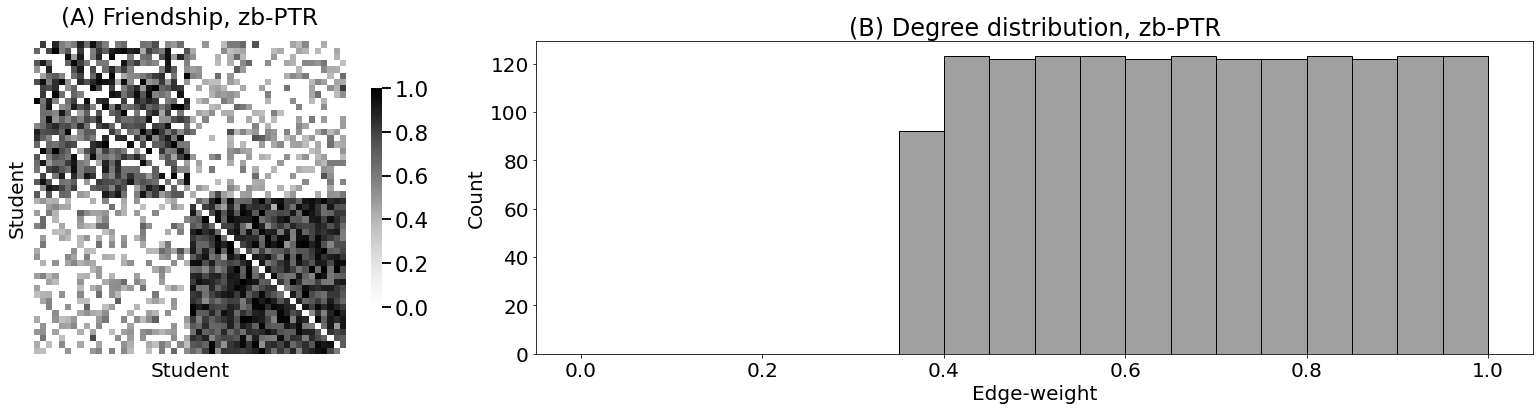
\includegraphics[width=\linewidth]{representations/ch4/Images/ptr_zb.png}
    \caption[Zero-Boosted PTR]{\textbf{(A)} the adjacency matrix, after zero-boosted\texttt{ptr}. \textbf{(B)} the edge-weight histogram, after zero-boosted\texttt{ptr}. Compare this to Figure \ref{fig:ch4:ptr}(B) and \ref{fig:ch4:ptr}(D), respectively.}
    \label{fig:ch4:ptr_zb}
\end{figure}

\paragraph{Thresholding as a decimation of ranking}
As it turns out, the thresholding approach you learned in Section \ref{sec:ch4:regularization:thresholding} can be thought of as a \emph{decimation} of ranking, assuming that the ranking implementation handles ties randomly (the implementation in\texttt{graspologic} does not, as ties are settled by the average rank, but we would encourage you to implement one that \emph{does} as an exercise). For instance, if you picked a threshold of $0.5$, there is some corresponding rank (or value in between two ranks), where all of the elements of the adjacency matrix with a rank lower than a given threshold $\tau_r$ have corresponding weights lower than $\tau$ and all of the elements of the adjacency matrix with a rank higher than a given threshold $\tau_r$ have corresponding weights higher than $\tau$. Then, you can simply threshold the ranked adjacency matrix using $\tau_r$.

\paragraph{Logging reduces magnitudinal differences between edges}
\label{sec:ch4:regularization:logscale}

When we look at the distribution of non-zero edge-weights for the activity/hobby network or the friendship network, we notice a strange pattern, known as a \emph{right-skew}. This is shown in Figure \ref{fig:ch4:log}(A). Informally, a distribution is \emph{right-skewed} if a large fraction of the points take relatively small values, and then a small portion of the points take relatively large values. Notice in this figure, for instance, that most points have an edge weight between $0$ and $2$, but and a small portion of points have an edge-weight between $2$ and $10$. This is called a ``right-skew'' because the histogram ``tails off'' as the values go to the right (increase). 


What if you want to make these large values more similar in relation to the smaller values, but you simultaneously want to preserve properties of the underlying distribution of the edge-weights? Well, you can't use\texttt{ptr`, because `ptr} will throw away all of the information about the edge-weight distribution other than the ordinal relationship between pairs of edges. To interpret what this means, you might think that there is a big difference between sharing no interests compared to three interests in common, but there is not as much of a difference in sharing ten interests compared to thirteen interests in common.

To do this, we instead turn to the logarithm function. The logarithm function $log_{10}(x)$ is defined for positive values $x$ as the value $c_x$ where $x = 10^{c_x}$. In this sense, it is the "number of powers of ten" to obtain the value $x$. The logarithm function is shown in Figure \ref{fig:ch4:log}(B).

\begin{figure}
    \centering
    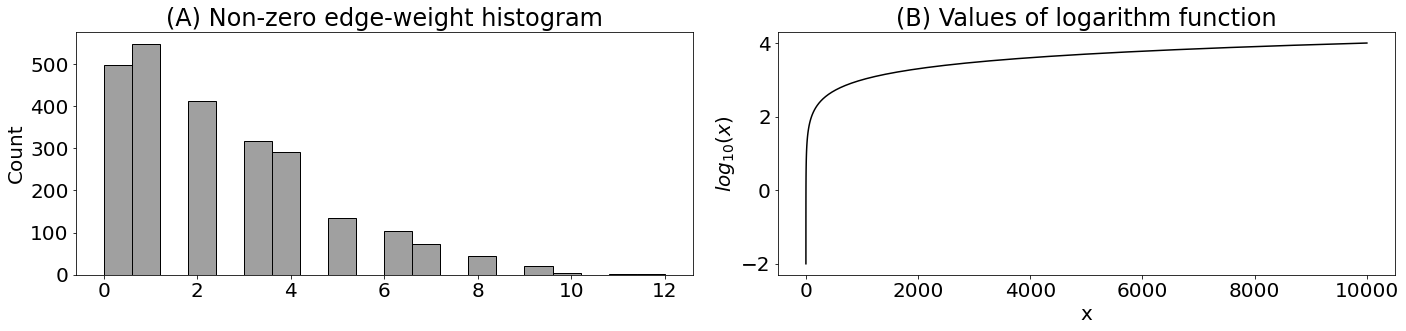
\includegraphics[width=\linewidth]{representations/ch4/Images/log.png}
    \caption[Heavy tailed edge-weights]{\textbf{(A)} The non-zero edge-weight histogram for the activity/hobby network. Notice that the histogram ``tails off'' towards the right. \textbf{(B)} The value for the base-$10$ logarithm function for given values of $x$.}
    \label{fig:ch4:log}
\end{figure}

What is key to noice about this function is that, as $x$ increases, the log of $x$ increases by a \emph{decreasing} amount. Let's imagine you have three values, $x = .001$, $y = .1$, and $z = 10$. A calculator will give you that $log_{10}(x) = -3, log_{10}(y) = -1$, and $log_{10}(z) = 1$. Even though $y$ is only $.099$ units bigger than $x$, its logarithm $log_{10}(y)$ exceeds $log_{10}(x)$ by two units. on the other hand, $z$ is $9.9$ units bigger than $y$, but yet its logarithm $log_{10}(z)$ is still the same two units bigger than $log_{10}(y)$. This is because the logarithm is instead looking at the fact that $z$ is \emph{one} power of ten, $y$ is $-1$ powers of ten, and $z$ is $-3$ powers of ten. The logarithm has \emph{collapsed} the huge size difference between $z$ and the other two values $x$ and $y$ by using exponentiation with \emph{base} ten. 


In this sense, you can also use the logarithm function for your network to reduce the huge size difference between the values in your activity/hobby network. However, we must first add a slight twist: to do this properly and yield an interpretable adjacency matrix, you need to \emph{augment} the entries of the adjacency matrix \emph{if} it contains zeros. This is because the $log_{10}(0)$ is \emph{not defined}. To augment the adjacency matrix, we'll basically ``inflate'' these values by a magnitude that is negligibly small. We show how to implement this in Algorithm \ref{alg:ch4:log_xfm}.

\begin{algorithm}[h]
    \SetAlgoLined
    \caption{Log transforming a network with zero-weight edges.}
    \KwData{$A$ is an adjacency matrix. \newline $b$ the base to log transform with.}
    \KwResult{The adjacency matrix, after log transformation.}

    Identify the entries of $A$ which take a value of zero.

    Identify the smallest entry of $A$ which is not-zero, and call it $a_m$.

    Compute a value $\epsilon$ which is an \emph{order of magnitude} smaller than $a_m$. Since you are taking powers of $b$, a single order of magnitude would give us that $\epsilon = \frac{a_m}{b}$. 

    Take the augmented adjacency matrix $A'$ to be defined with entries $a_{ij}' = a_{ij} + \epsilon$.

    Log transform $A'$ with a base of $b$.
\end{algorithm}

The first process of this procedure is called a \emph{zero augmentation}. We can code up the log transformation as follows:


\begin{lstlisting}[style=python]
def augment_zeros(X, base=10):
    if np.any(X < 0):
        raise TypeError("The logarithm is not defined for negative values!")
    am = np.min(X[np.where(X > 0)])  # the smallest non-zero entry of X
    eps = am/base  # epsilon is one order of magnitude smaller than the smallest non-zero entry
    return X + eps  # augment all entries of X by epsilon
def log_transform(X, base=10):
    """
    A function to log transform an adjacency matrix X, which may
    have zero-weight edges.
    """
    X_aug = augment_zeros(X, base=base)
    return np.log(X_aug)/np.log(base)

A_activity_log = log_transform(A_activity)
\end{lstlisting}

We plot the untransformed and log-transformed activity/hobby network in Figure \ref{fig:ch4:log_xfm}. 

When you plot the augmented and log-transformed data, what you see is that many of the edge-weights you originally might have thought were zero if you only looked at a plot were, in actuality, \emph{not} zero. In this sense, for non-negative weighted networks, log transforming after zero-augmentation is often very useful for visualization to get a sense of the magnitudinal differences that might be present between edges, since you can get a better feel for how different the big weights are from the smaller weights.

\begin{figure}[h]
    \centering
    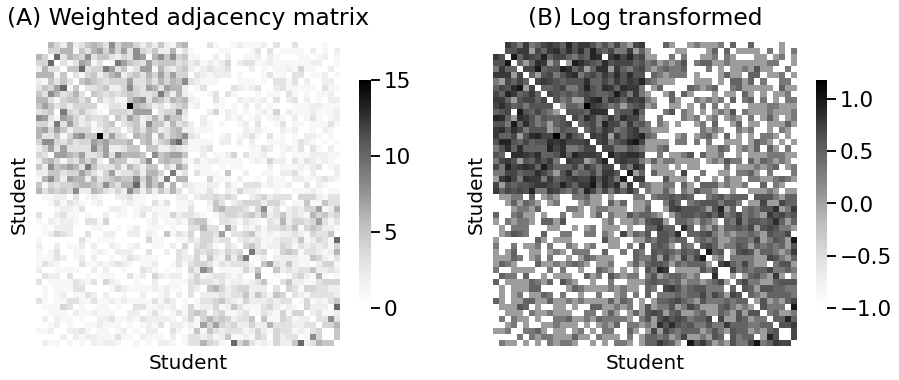
\includegraphics[width=\linewidth]{representations/ch4/Images/log_xfm.png}
    \caption[Log-transforming heavy-tailed edge-weights]{\textbf{(A)} The weighted adjacency matrix for the activity/hobby network. Notice that there are many entries which are very small, and it is hard to discern which entries are zero from the entries that are just tiny. \textbf{(B)} The activity/hobby network, after log transformation. Notice that the edges which are zero are readily apparent in the plot, and we have a better sense of the range of non-zero elements visually as well (they tend to fall between $0$ and $1$, so are different by approximately a power of $10$).}
    \label{fig:ch4:log_xfm}
\end{figure}


\bibliographystyle{vancouver}
\bibliography{references}